\chapter{中厚板剪切自锁问题}
本章针对中厚板剪切自锁问题,提出了有限元无网格混合离散分析方法最优约束比例。首先介绍了中厚板问题的混合离散过程,
其次对比中厚板问题的最优约束比例和传统约束比例。最后通过算例验证该方法的计算精度。
\section{中厚板问题}                  
考虑如图\ref{Mindlinplate}所示中厚板,其中中板厚为$h$,$\Omega$为板中面。在Mindlin假设下,中厚板考虑横向剪切变形,在纯受弯时平衡方程具有如下形式:
\begin{equation}\label{z-1}
\begin{cases}
    M_{\alpha\beta,\beta} - Q_\alpha = 0 & \textrm{in}\; \Omega \\
    Q_{\alpha,\alpha} + \bar q = 0 & \textrm{in}\; \Omega \\
    Q_\alpha n_\alpha = \pmb{\bar Q} & \textrm{on}\; \Gamma_Q \\
    M_{\alpha\beta} n_\beta = \pmb{\bar M}_\alpha & \textrm{on}\; \Gamma_M \\
    \varphi_\alpha = \bar \varphi_\alpha & \textrm{on}\; \Gamma_\varphi \\
    w = \bar w & \textrm{on}\; \Gamma_w \\
    \end{cases}
\end{equation}
\begin{figure}[H]
    \centering 
        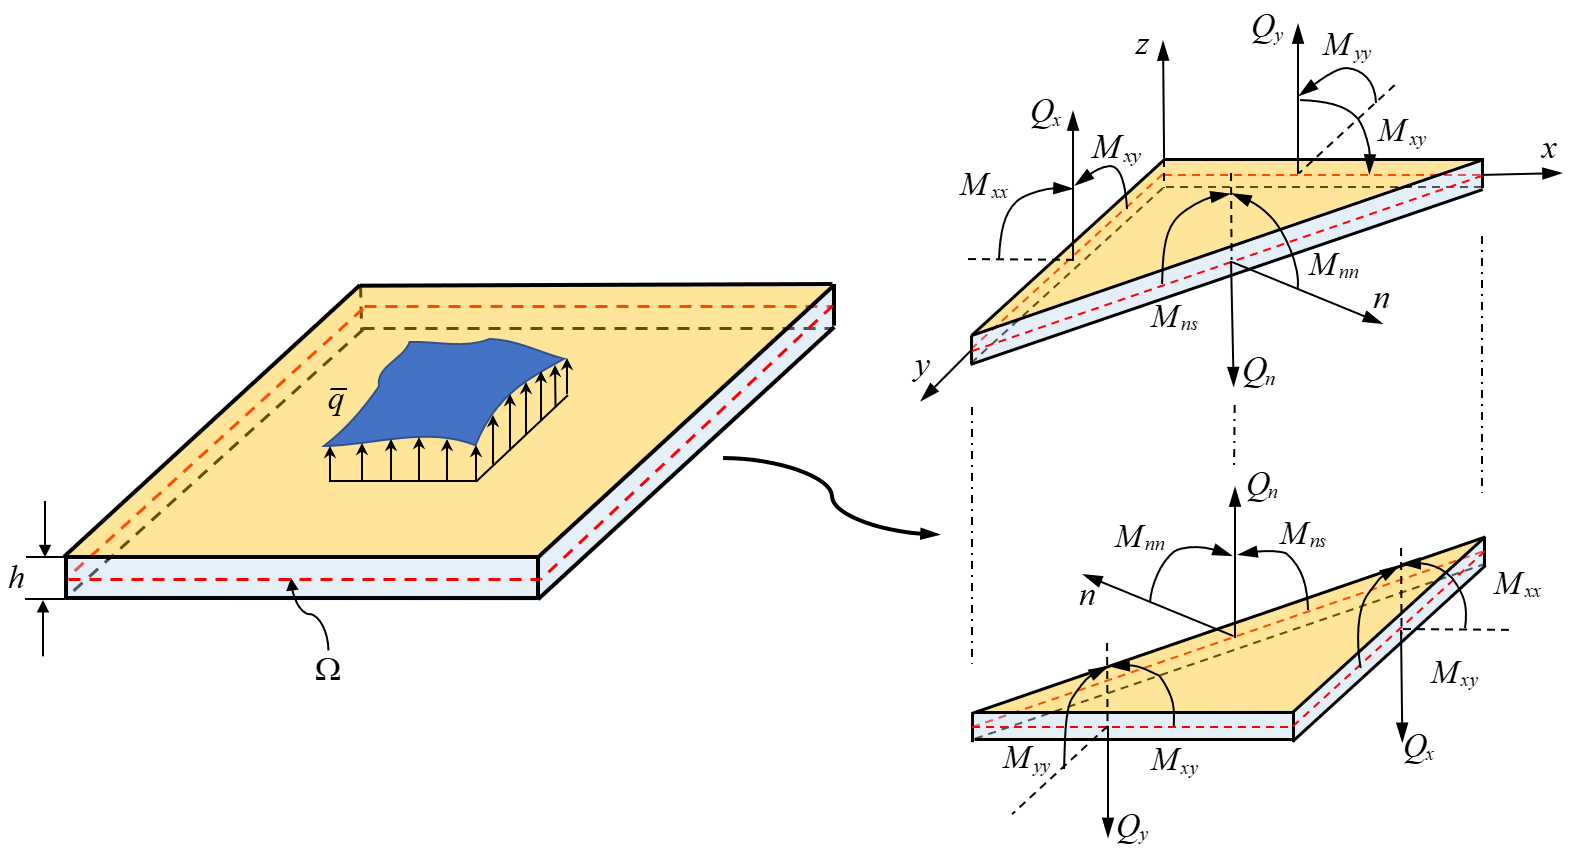
\includegraphics[scale=0.5]{figures/shearlocking/Mindlinplate.png}
        \caption{中厚板运动学及边界条件}\label{Mindlinplate}
\end{figure}
式中,$M_{\alpha \beta}$ 可表示弯矩张量$\pmb{M}$ 的弯曲或扭转部分的分量,$\bar{q}$ 为垂直于板中面的分布荷载;
$\Gamma_w$和$\Gamma_\varphi$为本质边界条件,$\bar{w}$和$\bar{\varphi}_\alpha$分别为本质边界条件上给定的挠度和转角;
$\Gamma_Q$ 和$\Gamma_M$ 为自然边界条件,$\bar{\pmb Q}$和$\pmb{\bar{M}}_{\pmb{\alpha}}$ 为自然边界上的等效剪力和法向弯矩;
$n_\alpha$为边界上外法线方向$\pmb{n}$的分量。

在平面应力假设下,当中厚板为线弹性各同向性材料时,其本构关系为:
\begin{equation} 
    \begin{split}
    M_{\alpha \beta}=-\frac{h^3}{12}D_{\alpha \beta \gamma\eta}\kappa_{\gamma\eta}=\frac{h^3}{12}D_{\alpha \beta \gamma\eta}\varphi_{\gamma,\eta}
    \end{split}
\end{equation}
\begin{equation} 
    \begin{split}
    Q_{\alpha}=k\frac{Eh}{2(1+\nu)}\gamma_\beta=kGh(-\varphi_\beta+w_{,\beta})
    \end{split}
\end{equation}
其中$k$为剪切修正系数,$\kappa_{\alpha\beta}$为曲率张量$\pmb\kappa$的分量,$\gamma_\alpha$为剪切应变矢量$\pmb\gamma$的分量,表达式为:
\begin{equation} 
    \kappa_{\alpha\beta}=-\varphi_{\alpha,\beta},\gamma_\alpha=-\varphi_\alpha+w_{,\alpha}
\end{equation}
其中$D_{\alpha \beta \gamma\eta}$为在平面应力假设下四阶弹性张量的分量,表达式为:
\begin{equation} 
    D_{\alpha \beta \gamma\eta}=\frac{E}{1-\nu^2}(\nu\delta_{\alpha\beta}\delta_{\gamma\eta}+\frac{1}{2}(1-\nu)(\delta_{\alpha\gamma}\delta_{\beta\eta}+\delta_{\alpha\eta}\delta_{\beta\gamma}))
\end{equation}

根据最小势能原理,强形式(\ref{z-1})所对应的势能泛函表达式为: 
\begin{equation}\label{z-snfh}
\begin{split} 
    \Pi(w,\boldsymbol{\varphi})&=\frac{1}{2}\int_{\Omega}\kappa_{\alpha\beta}M_{\alpha\beta}d\Omega+\frac{1}{2}\int_{\Omega}\gamma_{\alpha}Q_{\alpha}d\Omega\\
    &+\int_{\Gamma_{M}}\pmb\varphi_{\pmb \alpha}\cdot{\bar{\pmb M}_{\pmb{\alpha}}}d\Gamma-\int_{\Gamma_{Q}}{w}\bar {\pmb Q}d\Gamma-\int_{\Omega} w\bar{q}d\Omega
\end{split}
\end{equation}
对式(\ref{z-snfh})进行变分可得弱形式:
\begin{equation}\label{z-rxs}
    \begin{split} 
        \delta\Pi(w,\boldsymbol{\varphi})&=\int_{\Omega}\delta\kappa_{\alpha\beta}M_{\alpha\beta}d\Omega+\int_{\Omega}\delta\gamma_{\alpha}Q_{\alpha}d\Omega\\
        &+\int_{\Gamma_{M}}\pmb\delta\varphi_{\pmb \alpha}\cdot{\bar{\pmb M}_{\pmb{\alpha}}}d\Gamma-\int_{\Gamma_{Q}}{\delta{w}}\bar {\pmb Q}d\Gamma-\int_{\Omega} \delta{w}\bar{q}d\Omega
    \end{split}
    \end{equation}

在数值分析中,挠度$w$和转角$\varphi$可以用形函数和节点系数近似:
\begin{equation}
    w^h(\boldsymbol x) = \sum_{I=1}^{n_p} N_I(\boldsymbol x) w_I, \quad
    \varphi^h_\alpha(\boldsymbol x) = \sum_{I=1}^{n_p} N_I(\boldsymbol x) \varphi_{\alpha I}
\end{equation}
相应的近似曲率$\pmb\kappa^h$和近似剪切应变$\pmb\gamma^h$可表示为:
\begin{equation}\label{z-qulv}
    \boldsymbol\kappa^h = 
    \begin{Bmatrix}
    \kappa^h_{11} \\ \kappa^h_{22} \\ 2\kappa^h_{12} 
    \end{Bmatrix} = -\sum_{I=1}^{n_p}
    \begin{bmatrix}
    0 & N_{I,1} & 0 \\ 0 & 0 & N_{I,2} \\ 0 & N_{I,2} & N_{I,1}
    \end{bmatrix}
    \begin{Bmatrix}
    w_I \\ \varphi_{1I} \\ \varphi_{2I}
    \end{Bmatrix} = - \sum_{I=1}^{n_p} \boldsymbol B^b_I \boldsymbol d_I
\end{equation}
\begin{equation}\label{z-jqyb}
    \boldsymbol\gamma^h = 
    \begin{Bmatrix}
    \gamma^h_1 \\ \gamma^h_2
    \end{Bmatrix} = \sum_{I=1}^{n_p}
    \begin{bmatrix}
    N_{I,1} & N_I & 0 \\
    N_{I,2} & 0 & N_I
    \end{bmatrix}
    \begin{Bmatrix}
    w_I \\ \varphi_{1I} \\ \varphi_{2I}
    \end{Bmatrix} = \sum_{I=1}^{n_p} \boldsymbol B^s_I \boldsymbol d_I
\end{equation}

将离散应变(\ref{z-qulv})(\ref{z-jqyb})代入到弱形式(\ref{z-rxs})中得到离散平衡控制方程:
\begin{equation}
    (\boldsymbol K^b + \boldsymbol K^s) \boldsymbol d = \boldsymbol f
\end{equation}
其中$\boldsymbol K^b$和$\boldsymbol K^s$是具有以下分量的刚度矩阵:
\begin{equation}
    \boldsymbol K^b_{IJ} = \frac{h^3}{12} \int_\Omega \boldsymbol B^{bT}_I \boldsymbol D \boldsymbol B^b_J d\Omega
\end{equation}
\begin{equation}
    \boldsymbol K^s_{IJ} = h \int_\Omega \boldsymbol B^{sT}_I kG \boldsymbol B^s_J d\Omega
\end{equation}
式中$\pmb{D}$为平面应力弹性矩阵,$\pmb{f}$为力矢量,其分量具有以下形式:
\begin{equation}
    \boldsymbol f_I = \int_{\Gamma_Q} N_I \bar{\boldsymbol Q} d\Gamma - \int_{\Gamma_M} N_I \bar{\boldsymbol M} d\Gamma + \int_\Omega N_I \bar{\boldsymbol q} d\Omega
\end{equation}
其中:
\begin{equation}
\bar{\boldsymbol Q} = 
\begin{Bmatrix}
\bar Q \\ 0 \\ 0
\end{Bmatrix},
\bar{\boldsymbol M} =
\begin{Bmatrix}
0 \\ \bar M_1 \\ \bar M_2
\end{Bmatrix},
\bar{\boldsymbol q} =
\begin{Bmatrix}
\bar q \\ 0 \\ 0
\end{Bmatrix}
\end{equation}

当厚度$h$减少时弯曲刚度远小于剪切刚度,导致无法正确模拟出单元的弯曲,产生剪切自锁现象。
\section{位移-应力混合离散}
为了缓解厚度减小引起的剪切自锁,引入与挠度和转角无关的剪切应力$\pmb{Q}$,对挠度、转角和剪切应力采用混合离散的方式进行近似。剪切应力分量$Q_\alpha$通过无网格形函数进行近似可表示为:
\begin{equation}\label{z-jqyl}
    Q^h_\alpha(\boldsymbol x) = \sum_{K=1}^{n_q} \Psi_K(\boldsymbol x) q_{\alpha K}
\end{equation}
其中$q_{\alpha K}$表示与无网格节点$\boldsymbol x_K$对应的节点系数。

引入剪切应力,根据最小势能原理,势能泛函的表达式可更改为:
\begin{equation}\label{z-2}
\begin{split} 
    \Pi(w,\boldsymbol{\varphi},\boldsymbol{Q})&=\int_{\bar\Omega}\frac{1}{2}\varepsilon_{ij}\sigma_{ij} d\Omega+\frac{1}{2}\int_{\Omega}Q_{\alpha}(\gamma_{\alpha}-\frac{Q_{\alpha}}{kGh})d\Omega-\int_{\Gamma^{t}} u_{i}t_{i}d\Gamma-\int_{\Omega} u_{i}b_{i}d\Omega\\
    &=\frac{1}{2}\int_{\Omega}(\kappa_{\alpha \beta}M_{\alpha \beta}+\gamma_{\alpha}Q_{\alpha})d\Omega+\frac{1}{2}\int_{\Omega}Q_{\alpha}(\gamma_{\alpha}-\frac{Q_{\alpha}}{kGh})d\Omega\\
    &+\int_{\Gamma_{M}}\pmb\varphi_{\pmb \alpha}\cdot{\bar{\pmb M}_{\pmb{\alpha}}}d\Gamma-\int_{\Gamma_{Q}}{w}\bar {\pmb Q}d\Gamma-\int_{\Omega} w\bar{q}d\Omega
\end{split}
\end{equation}
对式(\ref{z-2})进行变分可得弱形式:
\begin{equation} 
    \begin{split}
    &\delta\Pi(w,\boldsymbol\varphi,\boldsymbol{Q})\\
    &=\int_{\Omega}\delta\kappa_{\alpha \beta}M_{\alpha \beta}d\Omega+\frac{1}{2}\int_{\Omega}\delta\gamma_{\alpha}Q_{\alpha}d\Omega+\frac{1}{2}\int_{\Omega}\gamma_{\alpha}\delta{Q}_{\alpha}d\Omega+\frac{1}{2}\int_{\Omega}\delta\gamma_{\alpha}Q_{\alpha}d\Omega\\
    &+\frac{1}{2}\int_{\Omega}\gamma_{\alpha}\delta{Q}_{\alpha}d\Omega-\int_{\Omega}\frac{\delta{Q}_{\alpha}{Q}_{\alpha}}{kGh}d\Omega+\int_{\Gamma_{M}}\delta\pmb\varphi_{\boldsymbol \alpha}\cdot{\boldsymbol{\bar M}_{\boldsymbol{\alpha}}}d\Gamma-\int_{\Gamma_{Q}}\delta{w}\boldsymbol{\bar Q}d\Gamma+\int_{\Omega} \delta{w}\bar{q}d\Omega\\
    &=\int_{\Omega}\delta\kappa_{\alpha \beta}M_{\alpha \beta}d\Omega+\int_{\Omega}\delta\gamma_{\alpha}Q_{\alpha}d\Omega+\int_{\Omega}\gamma_{\alpha}\delta{Q}_{\alpha}d\Omega-\int_{\Omega}\frac{\delta{Q}_{\alpha}{Q}_{\alpha}}{kGh}d\Omega+\int_{\Gamma_{M}}\delta\pmb\varphi_{\boldsymbol \alpha}\cdot{\boldsymbol{\bar M}_{\boldsymbol{\alpha}}}d\Gamma\\
    &-\int_{\Gamma_{Q}}\delta{w}\boldsymbol{\bar Q}d\Gamma+\int_{\Omega} \delta{w}\bar{q}d\Omega\\
    &=0
    \end{split}
\end{equation}
由上式可得平衡方程:
\begin{equation}\label{z-3}
    \int_{\Omega}\delta\kappa_{\alpha \beta}M_{\alpha \beta}d\Omega+\int_{\Omega}\delta\gamma_{\alpha}Q_{\alpha}d\Omega=\int_{\Gamma_{Q}}\delta{w}\pmb{\bar Q}d\Gamma-\int_{\Omega} \delta{w}\bar{q}d\Omega-\int_{\Gamma_{M}}\delta\pmb\varphi_{\pmb \alpha}\cdot{\pmb{\bar M}_{\pmb{\alpha}}}d\Gamma
\end{equation}
\begin{equation}\label{z-4}
    \int_{\Omega}\gamma_{\alpha}\delta{Q}_{\alpha}d\Omega-\int_{\Omega}\frac{\delta{Q}_{\alpha}{Q}_{\alpha}}{kGh}d\Omega=0
\end{equation}
将采用有限元近似的曲率(\ref{z-qulv})、剪切应变(\ref{z-jqyb})和采用无网格近似的剪切应力(\ref{z-jqyl})带入到弱形式(\ref{z-3})、(\ref{z-4})中得离散的平衡方程:
\begin{equation} 
    \begin{bmatrix}\pmb{K}^{b}&\pmb{K}^{sq}\\{\pmb{K}^{sq}}^T&\pmb{K}^{qq}\end{bmatrix}
    \begin{Bmatrix}\pmb{d}\\\pmb{q}\end{Bmatrix}=
    \begin{Bmatrix}\pmb{f}\\\pmb{0}\end{Bmatrix}
\end{equation}
式中,刚度矩阵$\boldsymbol K^{sq}$,$\boldsymbol K^{qq}$的分量具体表达式如下:
\begin{equation} 
    \boldsymbol K^{sq}_{IK} = \int_\Omega \boldsymbol B^{sT}_I \Psi_K d\Omega
\end{equation} 
\begin{equation} 
    \boldsymbol K^{qq}_{KL} = -\frac{1}{kGh} \int_\Omega \Psi_K \Psi_L \boldsymbol 1 d\Omega
\end{equation}
其中$\boldsymbol 1$为二阶恒等张量。
\section{中厚板剪切自锁问题最优约束比}

\section{数值算例}
\subsection{固支方板问题}
如图\ref{plate}所示,一固支方板求解域为$\Omega=(0,1)\otimes(0,1)$,边长$L=1$,厚度$h=0.1$,$0.01$,$0.001$,材料系数分别为杨氏模量
$E=10.92\times10^6$、泊松比$\mu=0.3$板面内分布如图所示纵向非均布荷载:
\begin{equation} 
\begin{split} 
    &F(x,y) =\\
    &E*h^3/(12*(1-ν^2))*(12*y*(y-1)*(5*x^2-5*x+1)*(2*y^2\\
    &*(y-1)^2+x*(x-1)*(5*y^2-5*y+1))+12*x*(x-1)*(5\\
    &*y^2-5*y+1)*(2*x^2*(x-1)^2+y*(y-1)*(5*x^2-5*x+1)))
\end{split} 
\end{equation}
该问题的精确解为:
\begin{equation} 
    \begin{split} 
        &w(x,y) = 1/3*x^3*(x-1)^3*y^3*(y-1)^3-2*h^2/(5*(1-ν))*(y^3*(y-1)^3\\
        &*x*(x-1)*(5*x^2-5*x+1)+x^3*(x-1)^3*y*(y-1)*(5*y^2-5*y+1))\\
        &\theta_1(x,y) = y^3*(y-1)^3*x^2*(x-1)^2*(2*x-1)\\
        &\theta_2(x,y) = x^3*(x-1)^3*y^2*(y-1)^2*(2*y-1)
    \end{split} 
\end{equation}
\begin{figure}[H]
    \centering 
        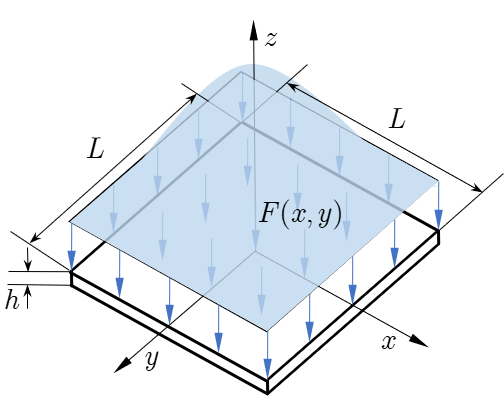
\includegraphics[scale=0.8]{figures/shearlocking/plate.png}
        \caption{固支方板问题模型}\label{plate}
\end{figure}
 
为研究误差收敛性,采用图\ref{platemsh}所示的均布的$9\times 9$、$17\times 17$、$33\times 33$、$65\times 65$
的四个疏密不同的节点进行离散,并采用线性单元:三角形三节点单元(Tri3)、四边形四节点单元(Quad4),二次单元:
三角形六节点单元(Tri6)、四边形八节点单元(Quad8)。此时对于采用对于线性基函数的固支方板问题其影响域取为1.5倍
的积分域长度,采用二次基函数时其影响域取为2.5倍积分域长度。

如图\ref{linear-l2}为固支方板问题线性单元位移误差对比图。从图中可以看出线性单元传统有限元方法在厚度为$0.1$时能
达到理论误差收敛率但计算精度低于混合离散法,在厚度为$0.01$,$0.001$时无法到达理论误差收敛率,产生了剪切自锁现象。
混合离散法在三个厚度均能达到理论误差收敛率。图\ref{quad-l2}为固支方板问题二次单元位移误差对比图。从图中可以看
出二次单元传统有限元方法在厚度为$0.1$时能达到理论误差收敛率且计算精度与混合离散方法相当,在厚度为$0.01$时能达到
理论误差收敛率但计算精度低于混合离散方法,在厚度为$0.001$时无法到达理论误差收敛率。
\begin{figure}[H]
    \centering 
    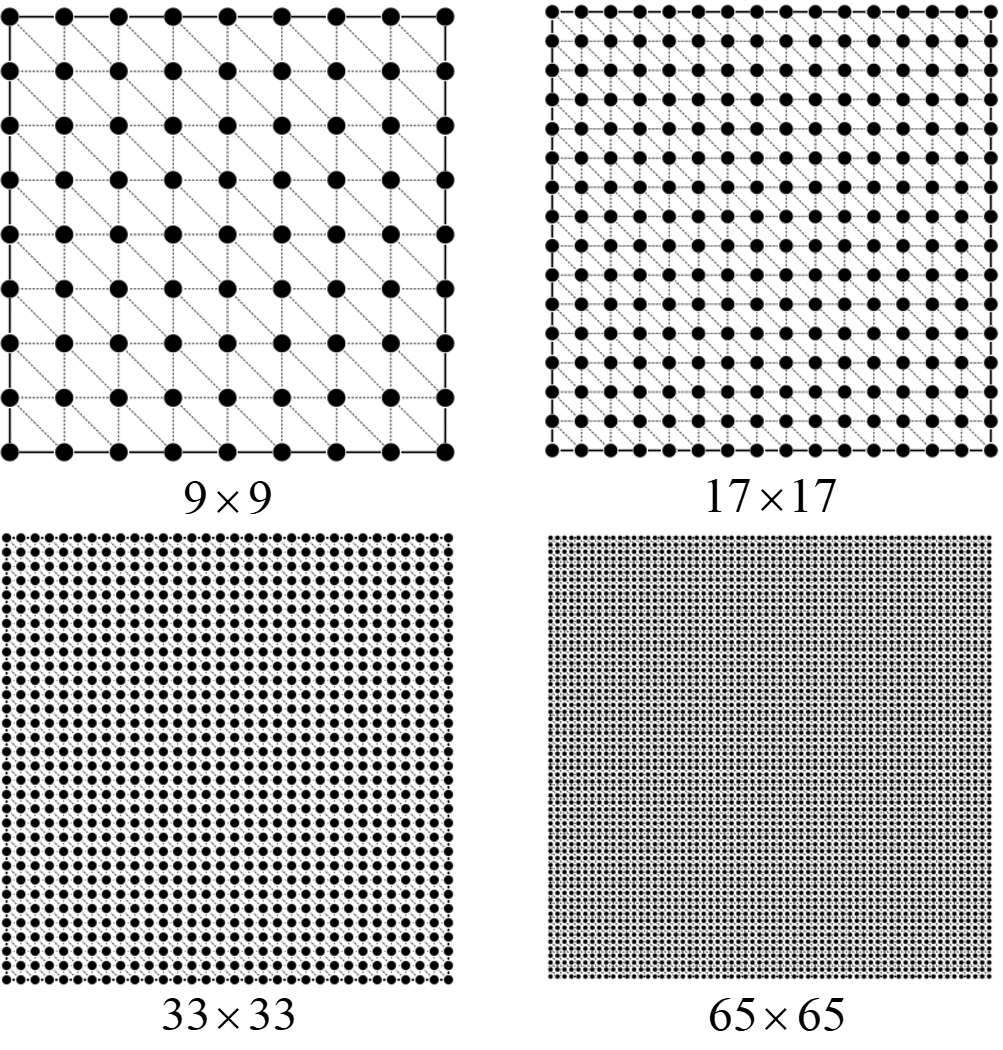
\includegraphics[scale=0.5]{figures/shearlocking/platemsh.png}
    \caption{固支方板问题节点离散}\label{platemsh}
\end{figure}
\begin{figure}[H]
    \centering
    \begin{subcaptiongroup}
    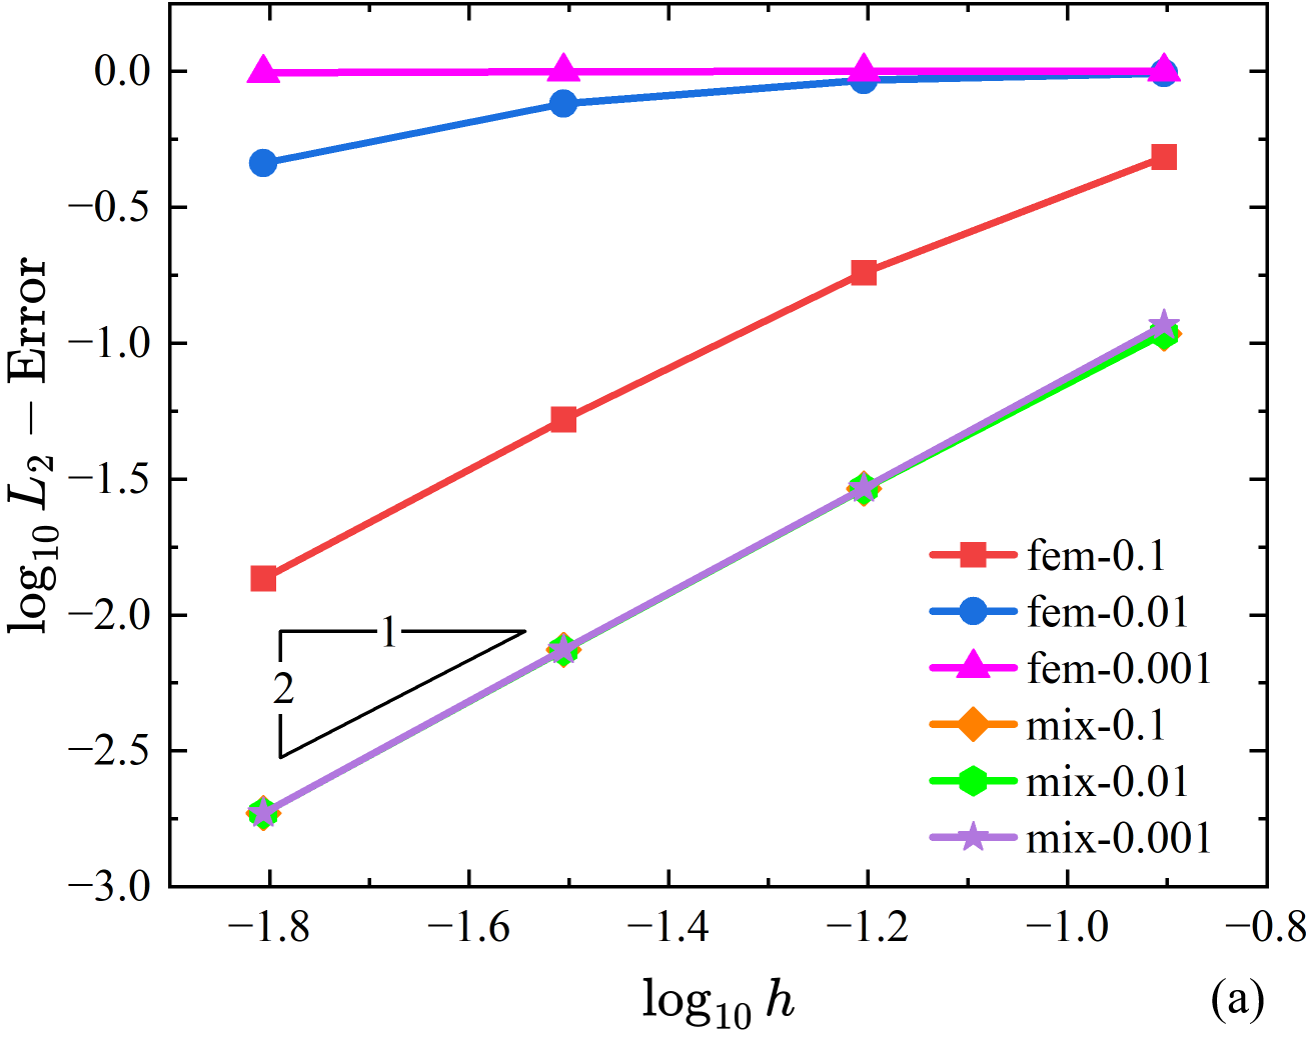
\includegraphics[width=0.49\textwidth]{figures/shearlocking/T3-l2-h.png}
    \phantomcaption\label{T3-l2-h}
    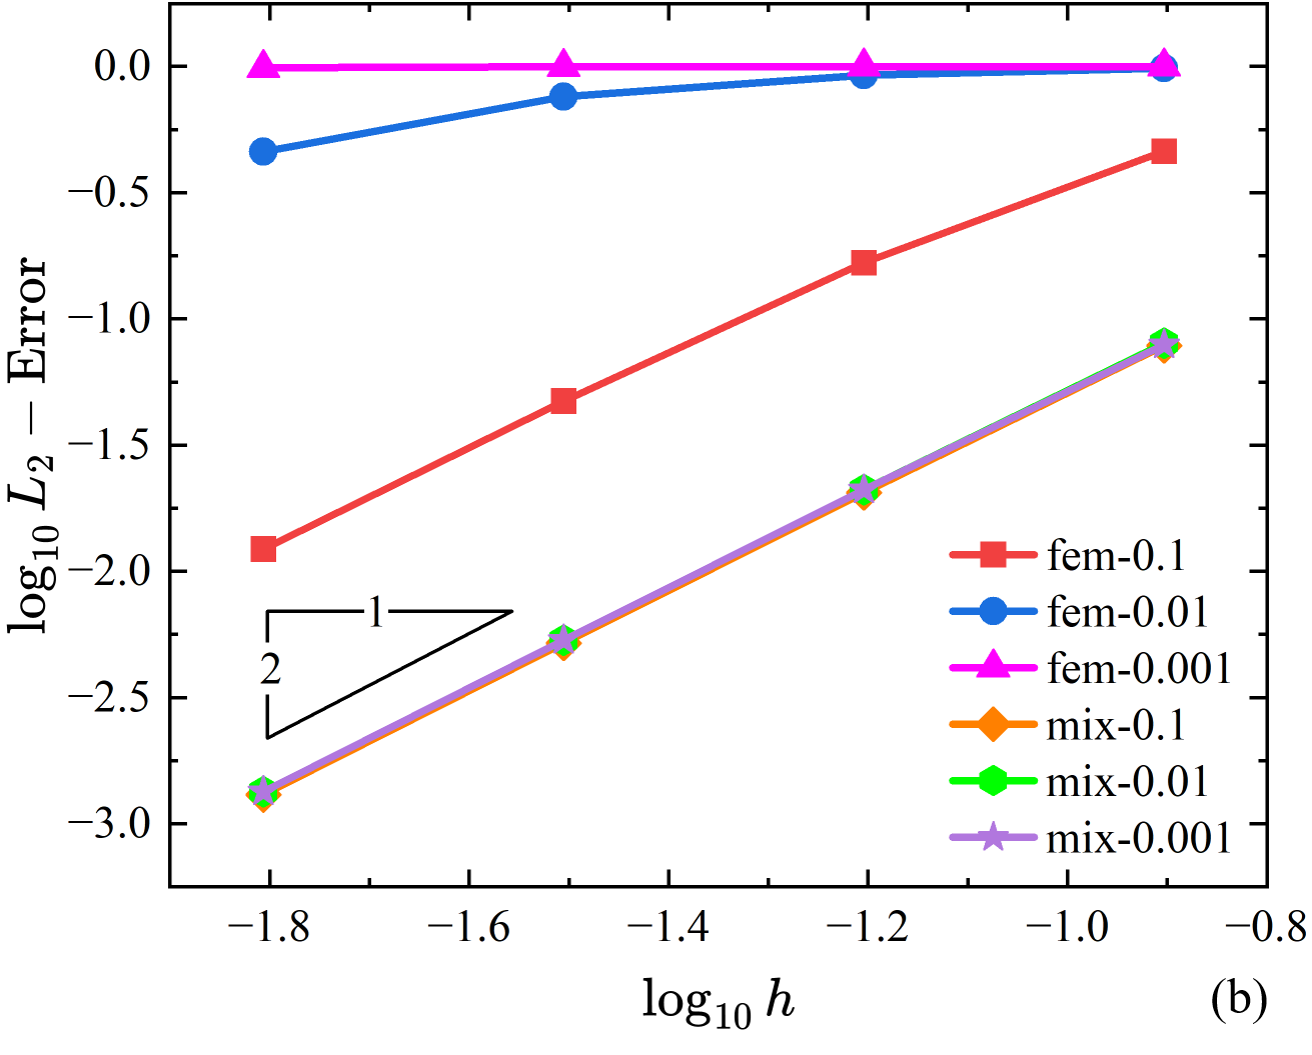
\includegraphics[width=0.49\textwidth]{figures/shearlocking/Q4-l2-h.png}
    \phantomcaption\label{Q4-l2-h}
    \end{subcaptiongroup}
\caption{\centering{固支方板问题线性单元误差对比:\protect\linebreak \subref{T3-l2-h} Tri3单元$L_2$误差;\subref{Q4-l2-h}Quad4单元 $L_2$误差}}
\label{linear-l2}
\end{figure}
\begin{figure}[H]
    \centering
    \begin{subcaptiongroup}
    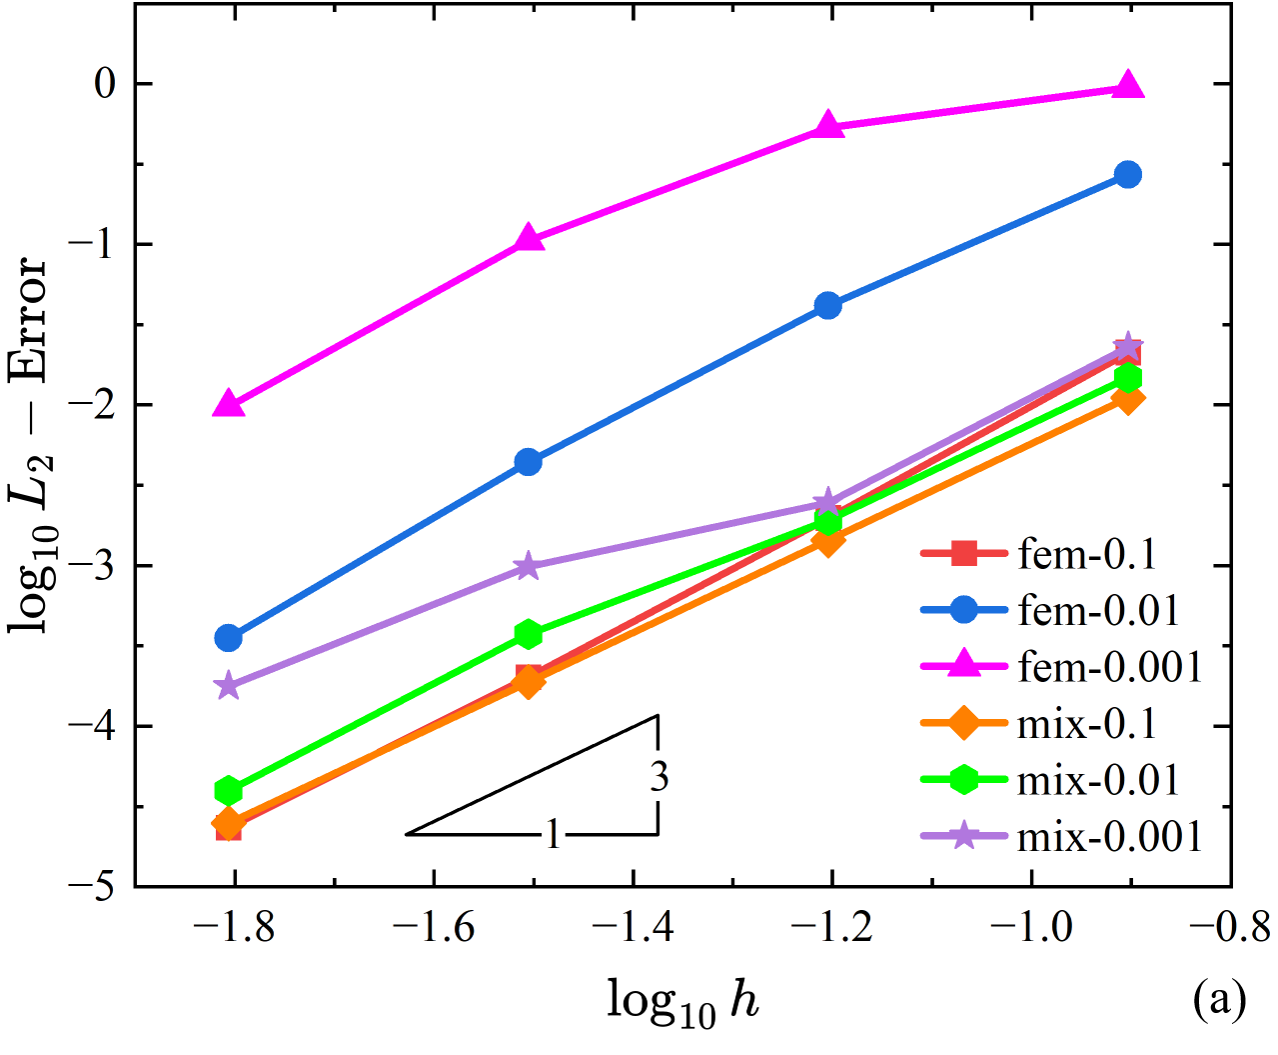
\includegraphics[width=0.49\textwidth]{figures/shearlocking/T6-l2-h.png}
    \phantomcaption\label{T6-l2-h}
    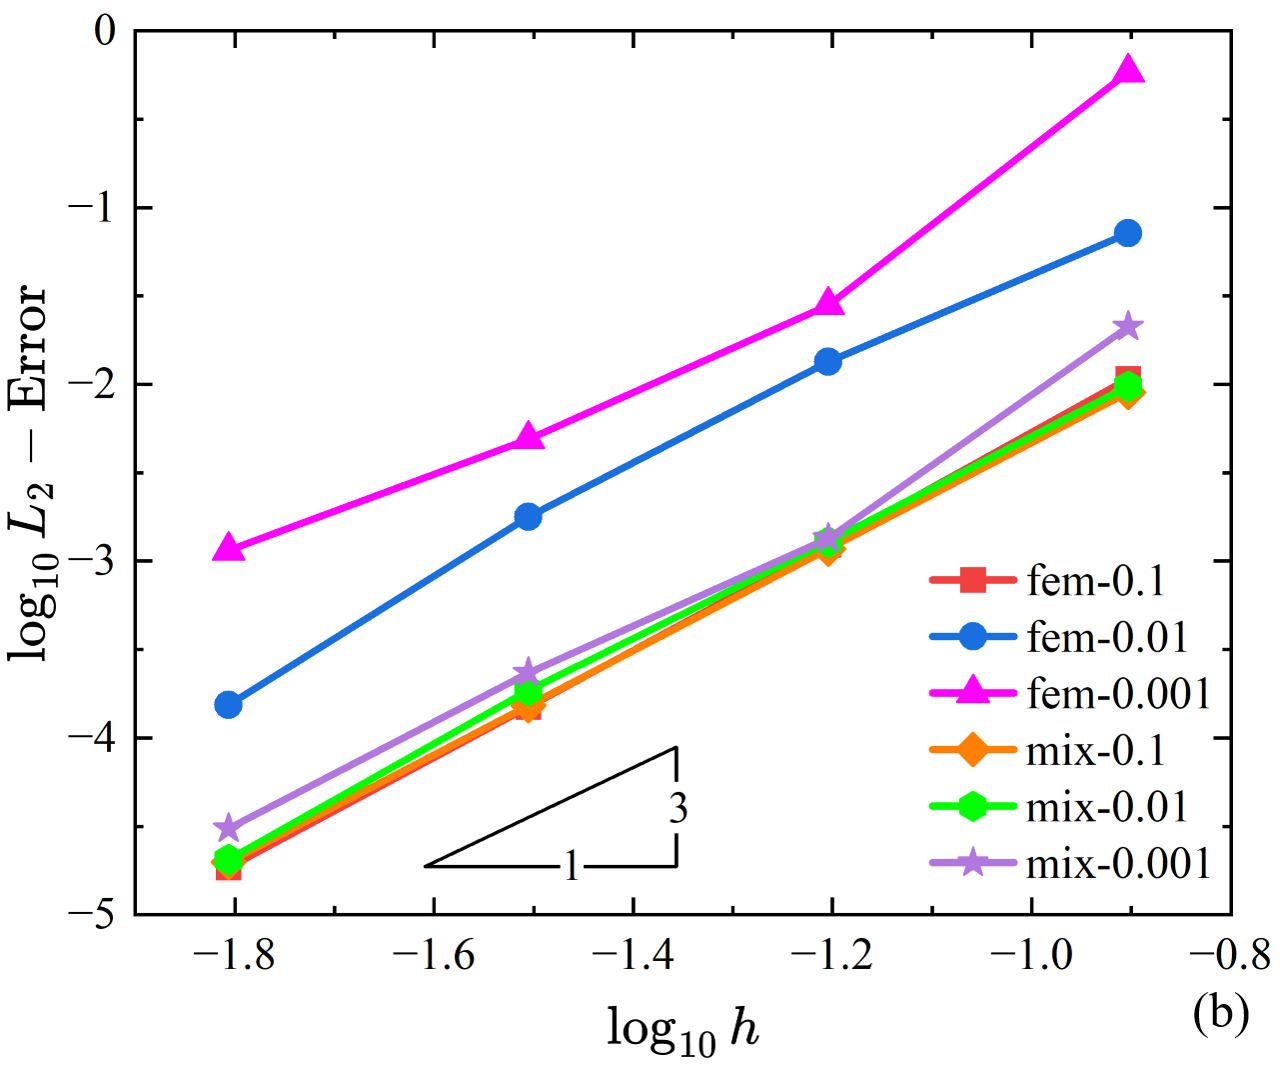
\includegraphics[width=0.49\textwidth]{figures/shearlocking/Q8-l2-h.png}
    \phantomcaption\label{Q8-l2-h}
    \end{subcaptiongroup}
\caption{\centering{固支方板问题二次单元误差对比:\protect\linebreak \subref{T6-l2-h} Tri6单元$L_2$误差;\subref{Q8-l2-h}Quad8单元 $L_2$误差}}
\label{quad-l2}
\end{figure}
位移分别采用图\ref{platemsh}所示的网格单元,通过改变剪切应力节点的数量,验证剪切应力节点数量与误差的关系。图\ref{linear-ns}、
\ref{quad-ns}为相对应的结果。图\ref{linear-ns}为线性单元剪切应力节点数量与误差的关系,其中Tri3单元和Quad4单元的位移节点数量一致。
图(a),(b)最优应力节点数为,分析结果显示,随着应力节点数量的减少位移误差率先达到最小值,而应力误差虽有所下降但其值始终保持在较高水平。
图(c),(d)和图(e)(f)的最优应力节点数分别为。分析结果显示,应力节点数量的减少位移误差同样先达到最小值。值得注意的是,在约束比
达到最优值附近时,应力误差也会随之达到最小值。图\ref{quad-ns}为二次单元剪切应力节点数量与误差的关系,图(a),(b)最优应力节点数分别为,
对于二次单元同样具有上述效果。这一现象在所有节点数量条件下均得到了验证。
\begin{figure}[H]
    \centering
    \begin{subcaptiongroup}
    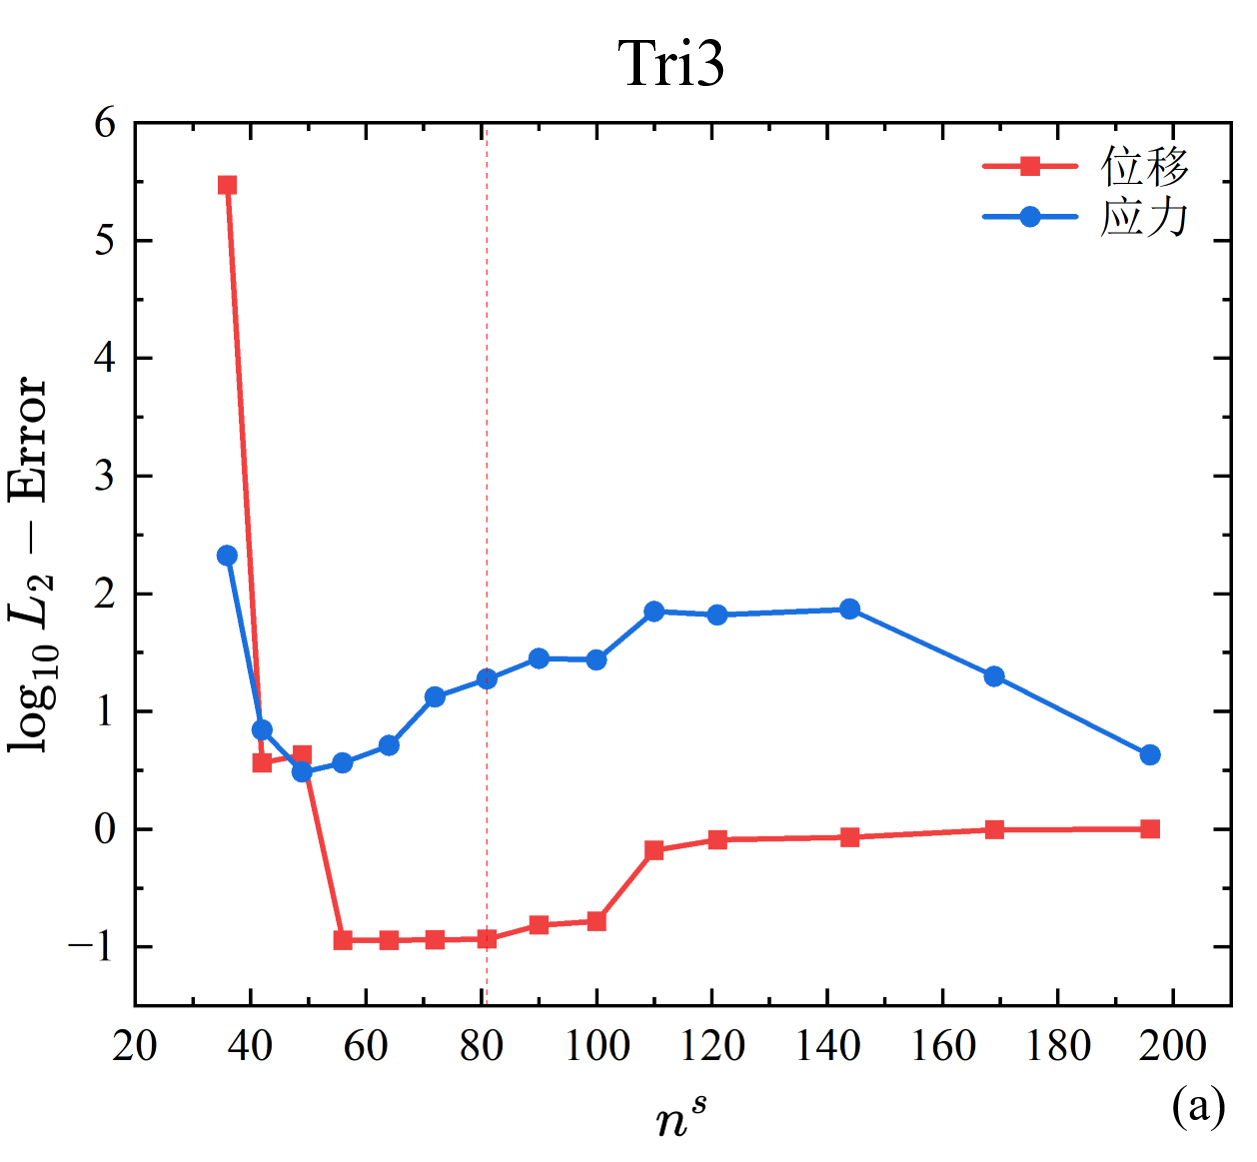
\includegraphics[width=0.48\textwidth]{figures/shearlocking/T3-l2-ns8.png}
    \phantomcaption\label{T3-l2-ns8}
    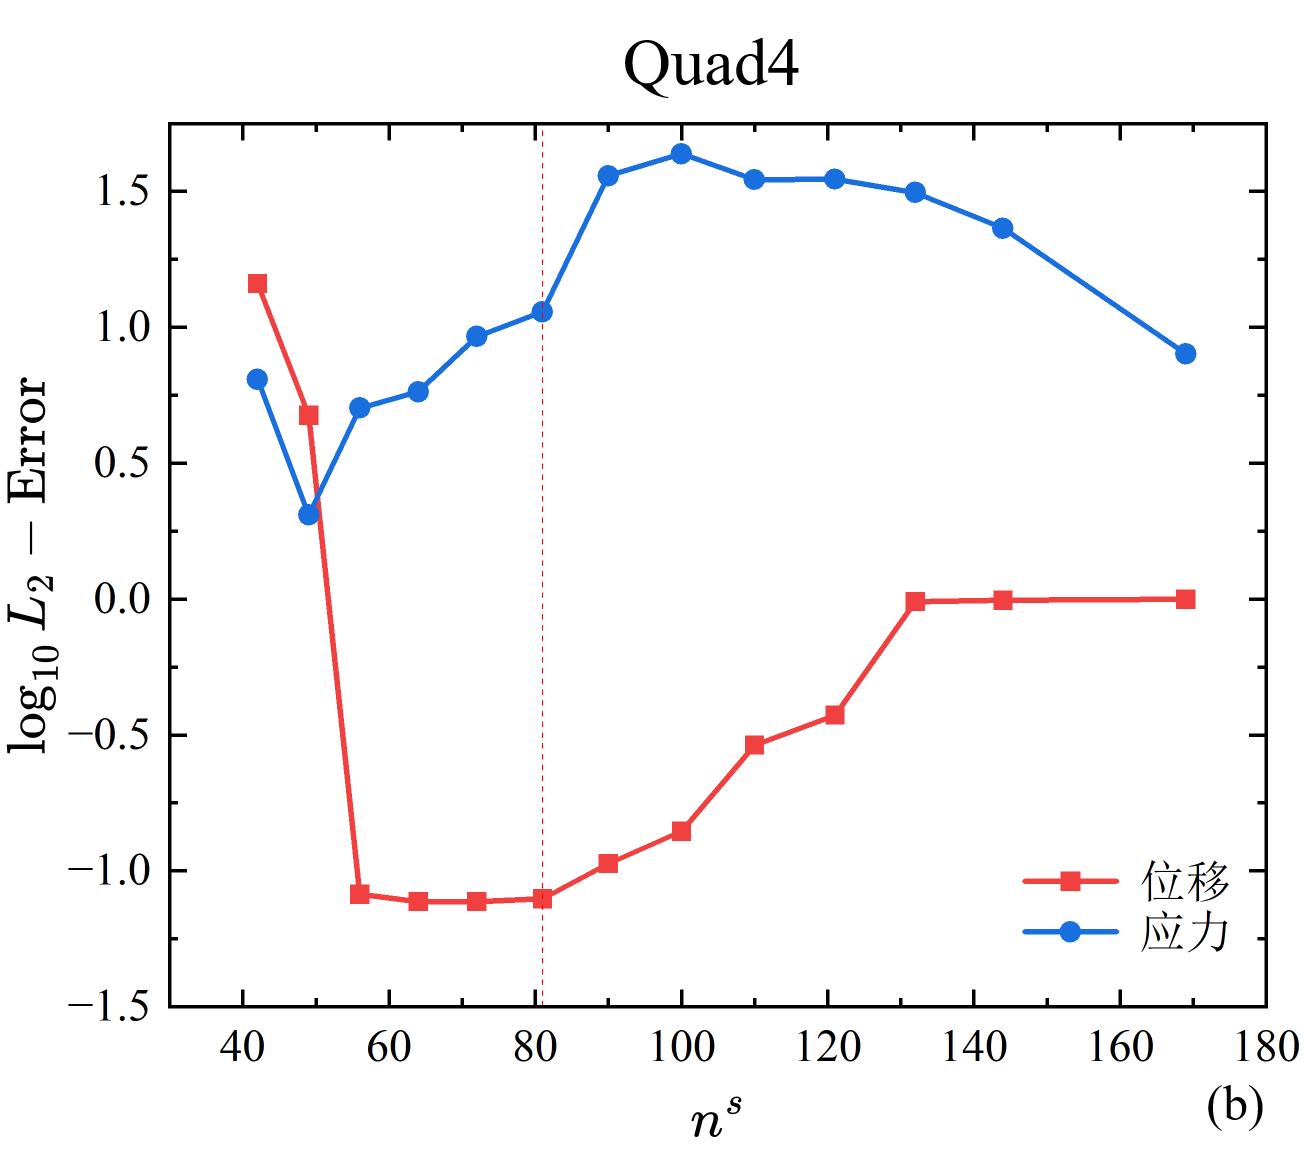
\includegraphics[width=0.50\textwidth]{figures/shearlocking/Q4-l2-ns8.png}
    \phantomcaption\label{Q4-l2-ns8}
    \end{subcaptiongroup}
    \begin{subcaptiongroup}
    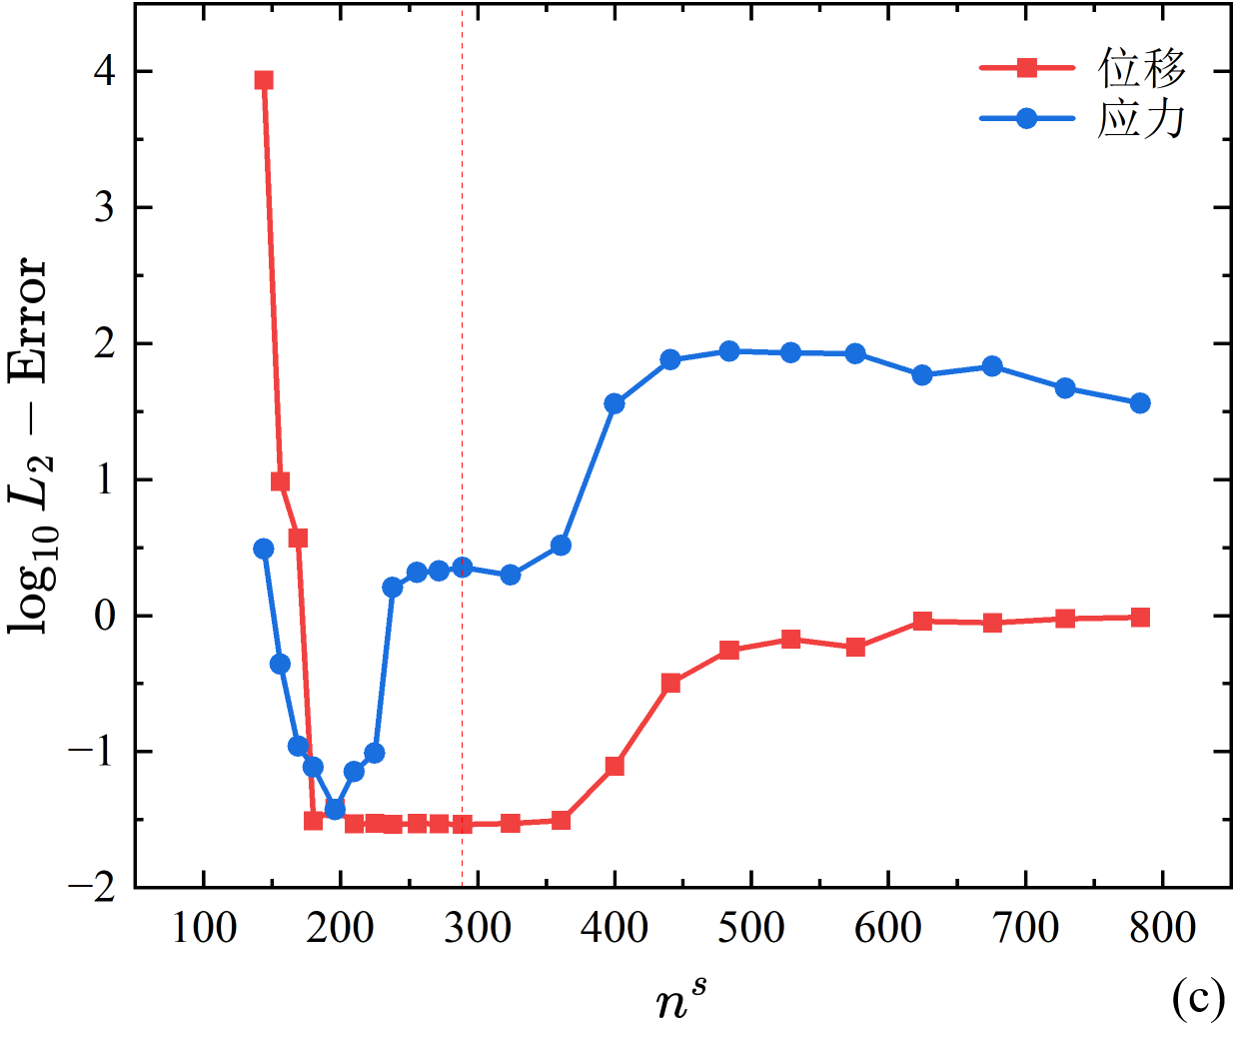
\includegraphics[width=0.49\textwidth]{figures/shearlocking/T3-l2-ns16.png}
    \phantomcaption\label{T3-l2-ns16}
    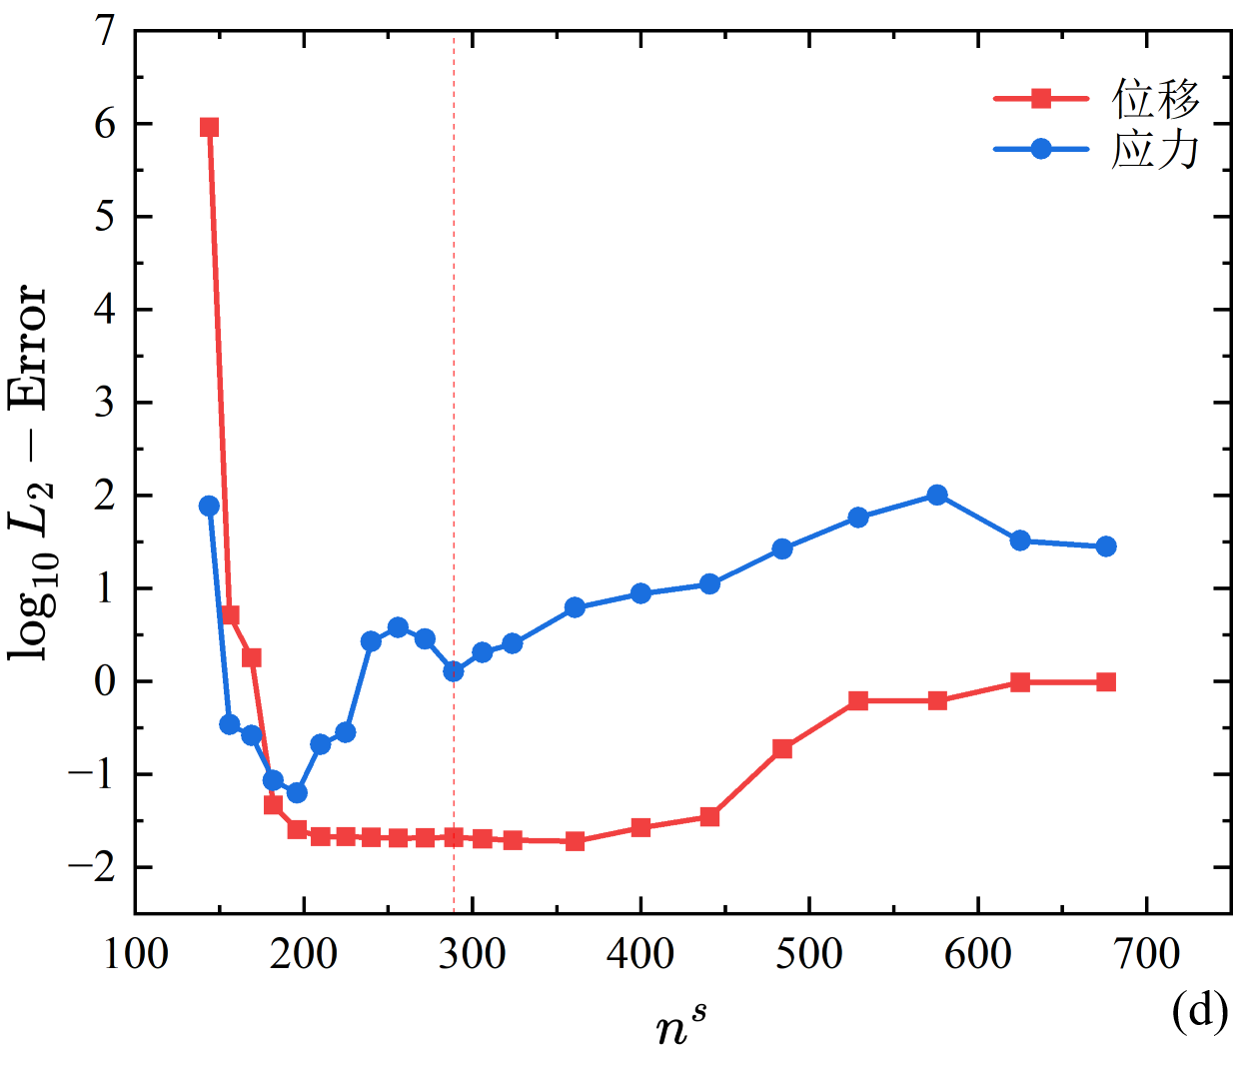
\includegraphics[width=0.49\textwidth]{figures/shearlocking/Q4-l2-ns16.png}
    \phantomcaption\label{Q4-l2-ns16}
    \end{subcaptiongroup}
    \begin{subcaptiongroup}
    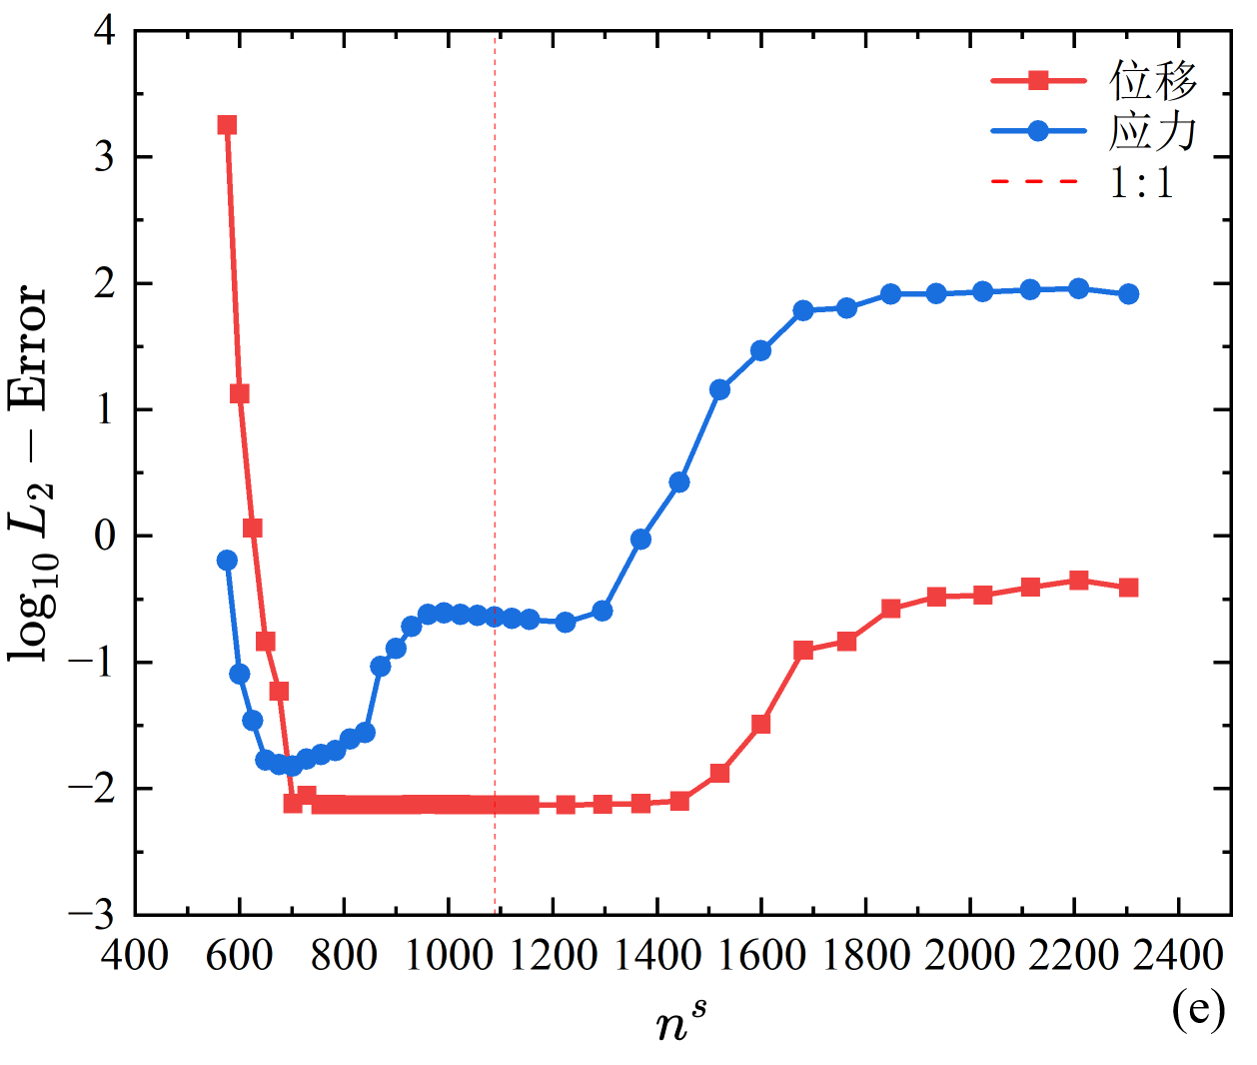
\includegraphics[width=0.49\textwidth]{figures/shearlocking/T3-l2-ns32.png}
    \phantomcaption\label{T3-l2-ns32}
    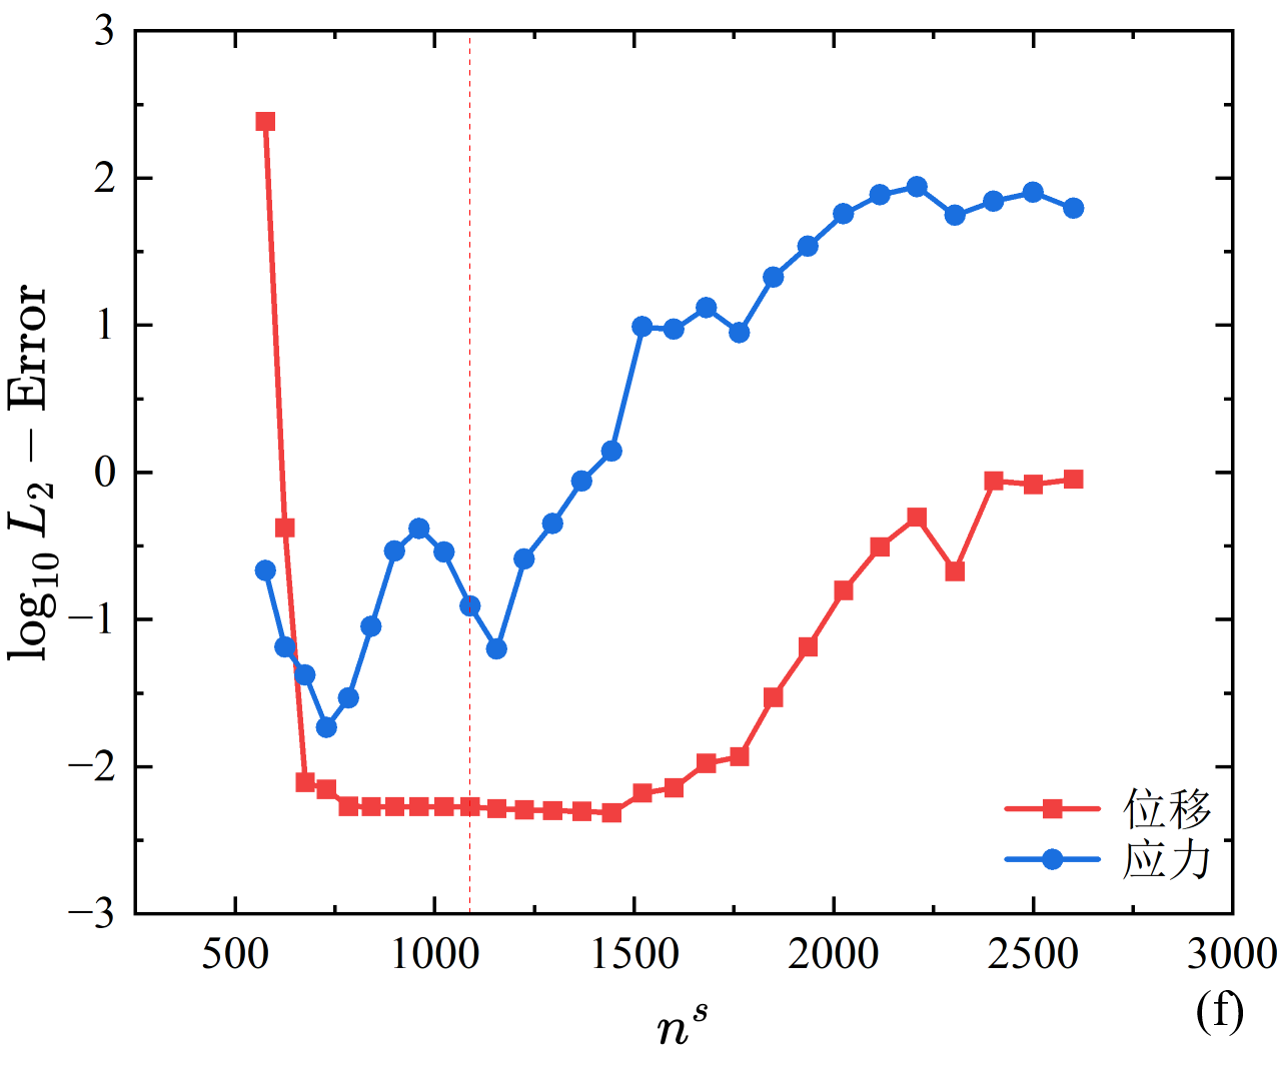
\includegraphics[width=0.49\textwidth]{figures/shearlocking/Q4-l2-ns32.png}
    \phantomcaption\label{Q4-l2-ns32}
    \end{subcaptiongroup}
\caption{\centering{固支方板问题线性单元$L2$误差与剪切应力节点数量的关系:\protect\linebreak
\subref{T3-l2-ns8},\subref{Q4-l2-ns8} $8\times 8$单元$L_2$误差; 
\subref{T3-l2-ns16},\subref{Q4-l2-ns16} $16\times 16$单元$L_2$误差;
\subref{T3-l2-ns32},\subref{Q4-l2-ns32} $32\times 32$单元$L_2$误差}}
\label{linear-ns}
\end{figure}

\begin{figure}[H]
    \centering
    \begin{subcaptiongroup}
    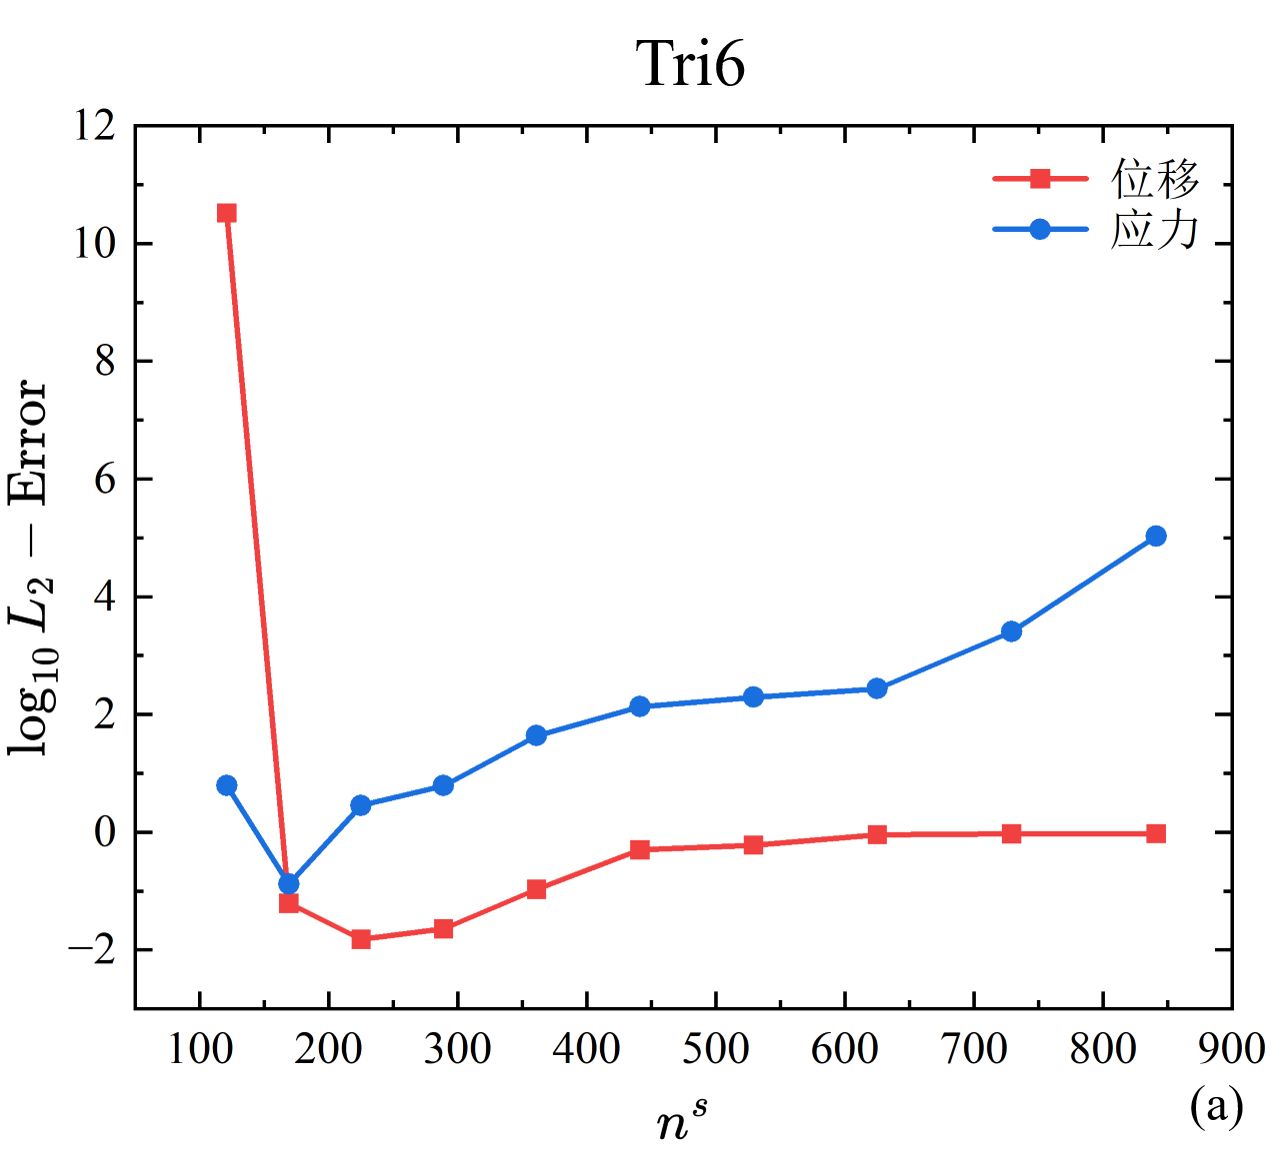
\includegraphics[width=0.49\textwidth]{figures/shearlocking/T6-l2-ns8.png}
    \phantomcaption\label{T6-l2-ns8}
    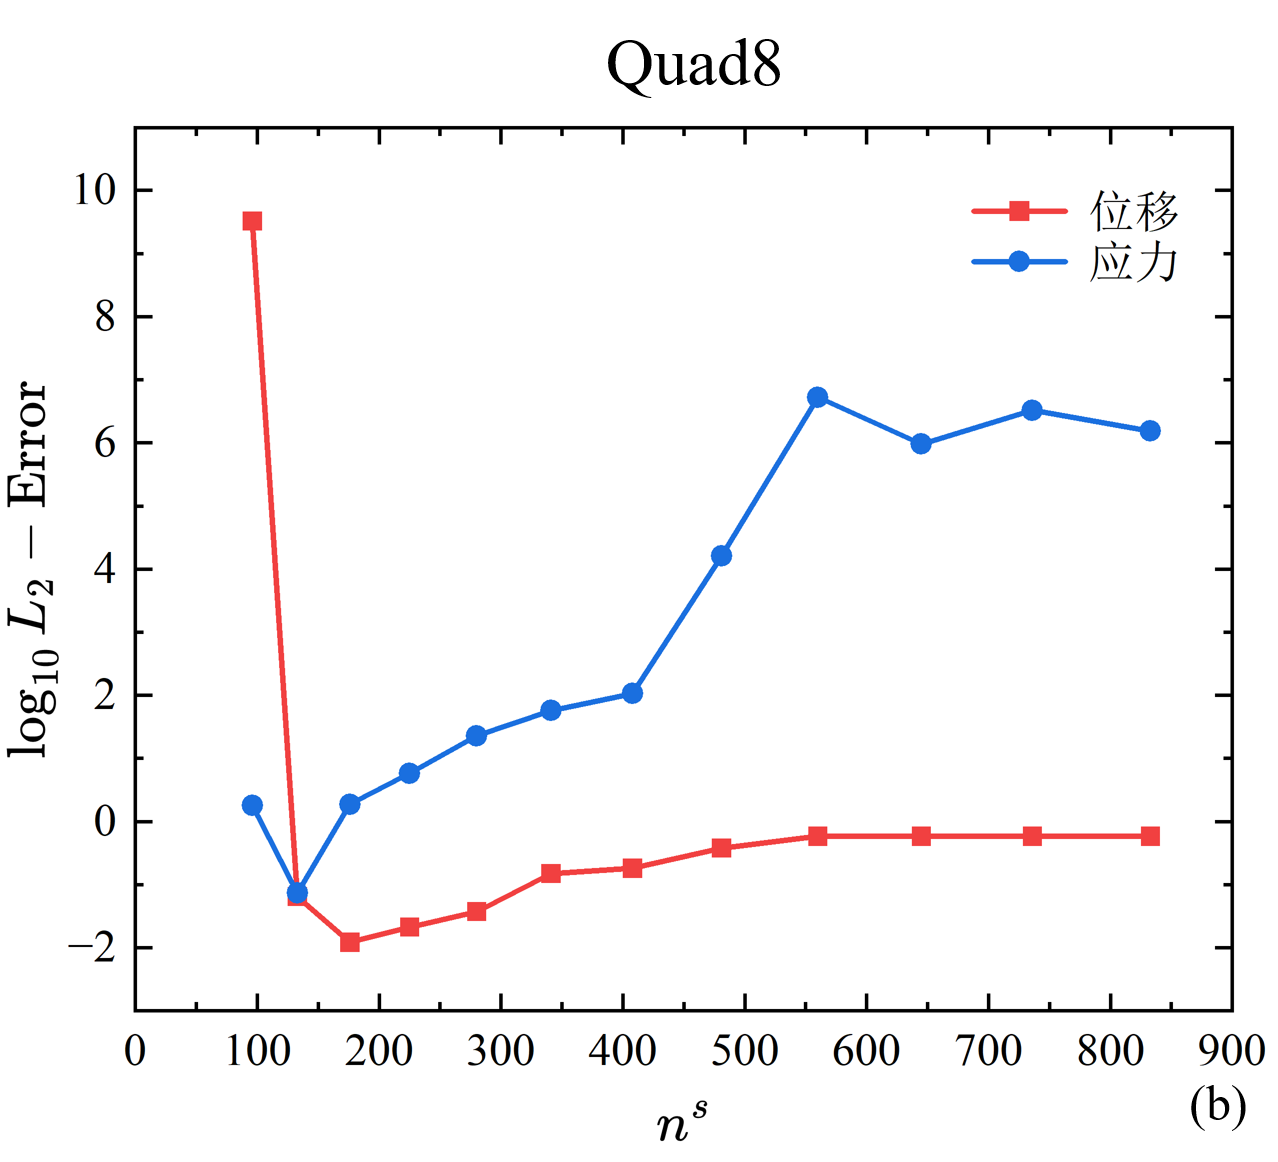
\includegraphics[width=0.49\textwidth]{figures/shearlocking/Q8-l2-ns8.png}
    \phantomcaption\label{Q8-l2-ns8}
    \end{subcaptiongroup}
    \begin{subcaptiongroup}
    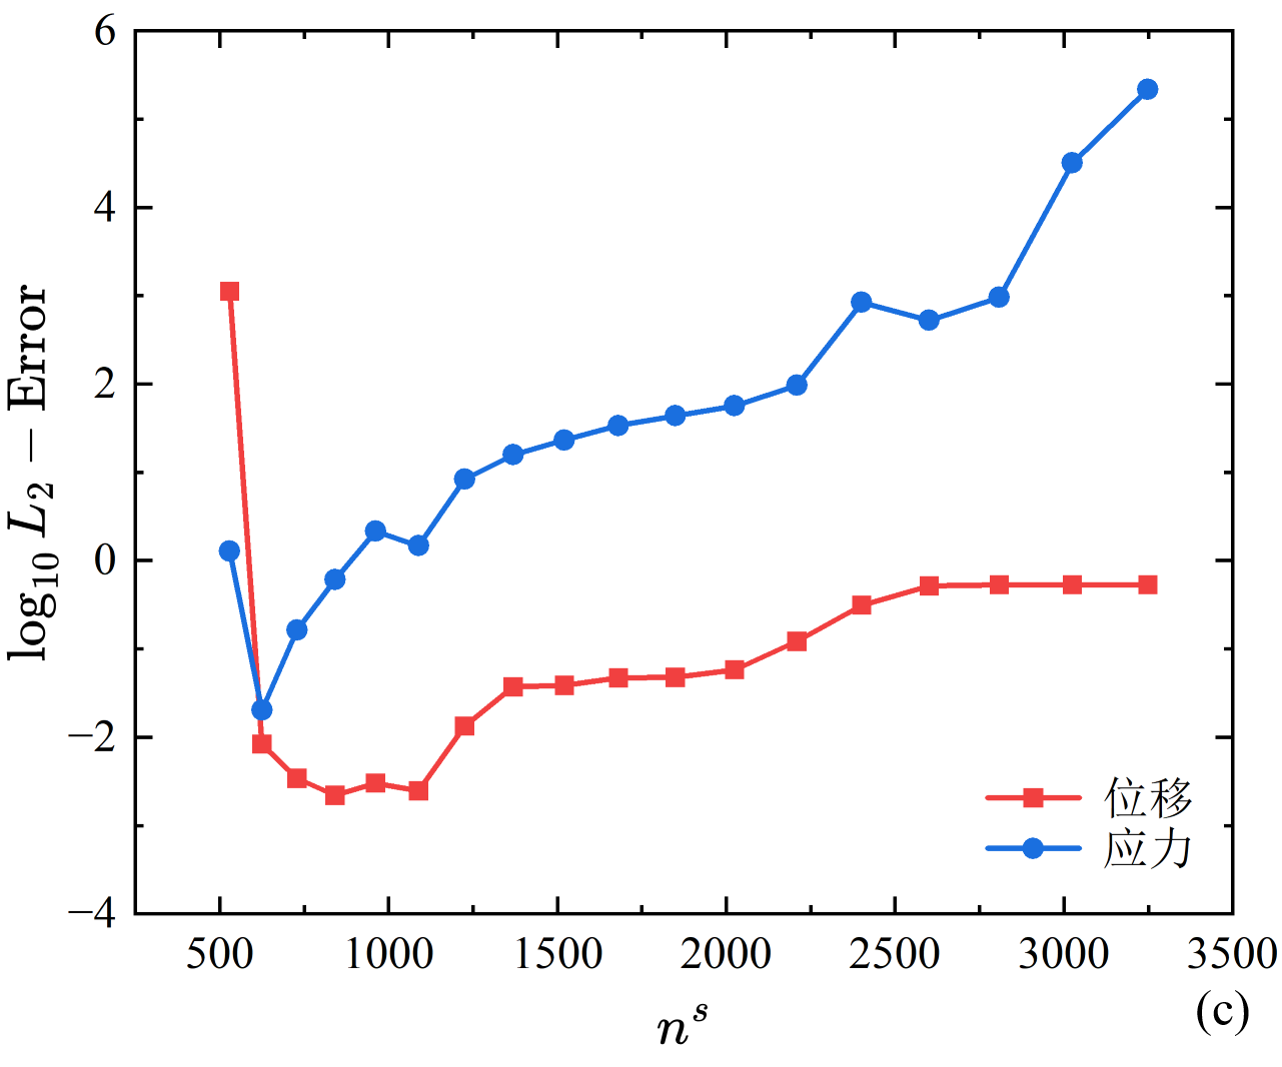
\includegraphics[width=0.49\textwidth]{figures/shearlocking/T6-l2-ns16.png}
    \phantomcaption\label{T6-l2-ns16}
    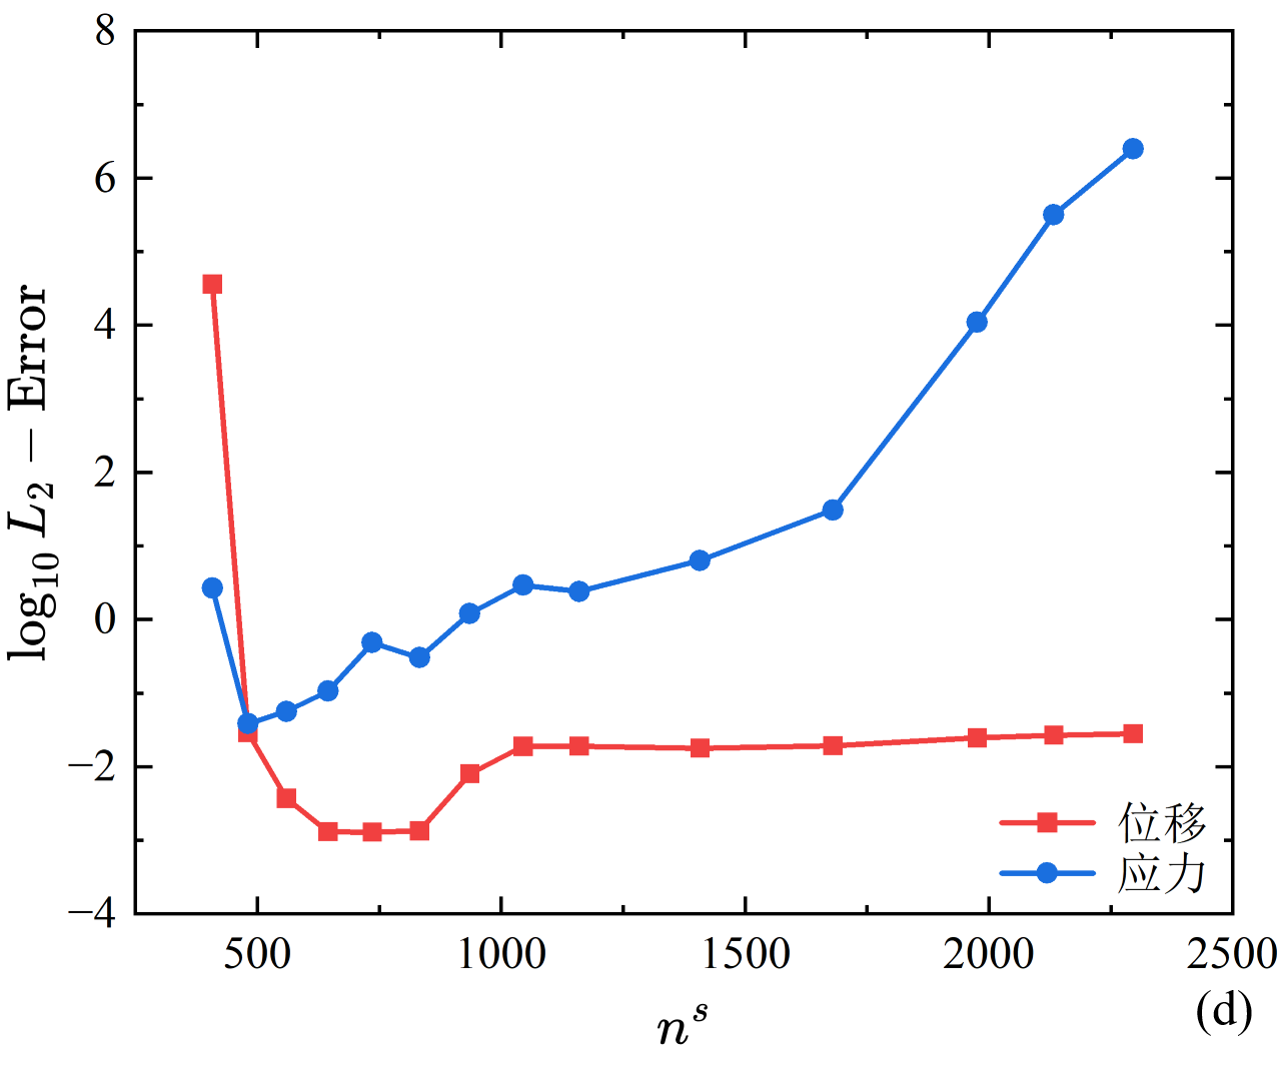
\includegraphics[width=0.49\textwidth]{figures/shearlocking/Q8-l2-ns16.png}
    \phantomcaption\label{Q8-l2-ns16}
    \end{subcaptiongroup}
    \begin{subcaptiongroup}
    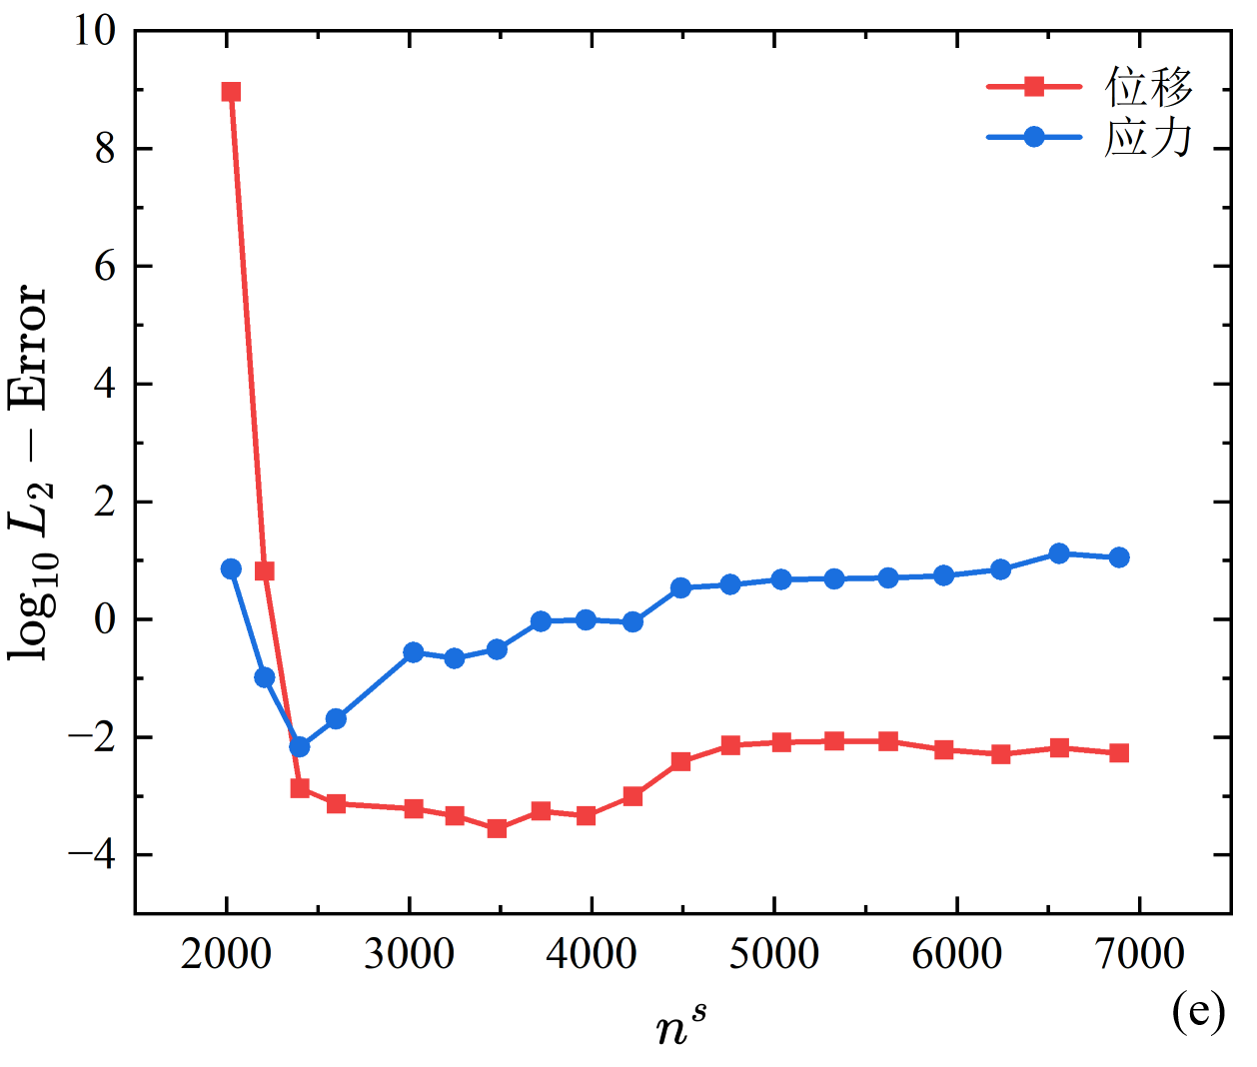
\includegraphics[width=0.49\textwidth]{figures/shearlocking/T6-l2-ns32.png}
    \phantomcaption\label{T6-l2-ns32}
    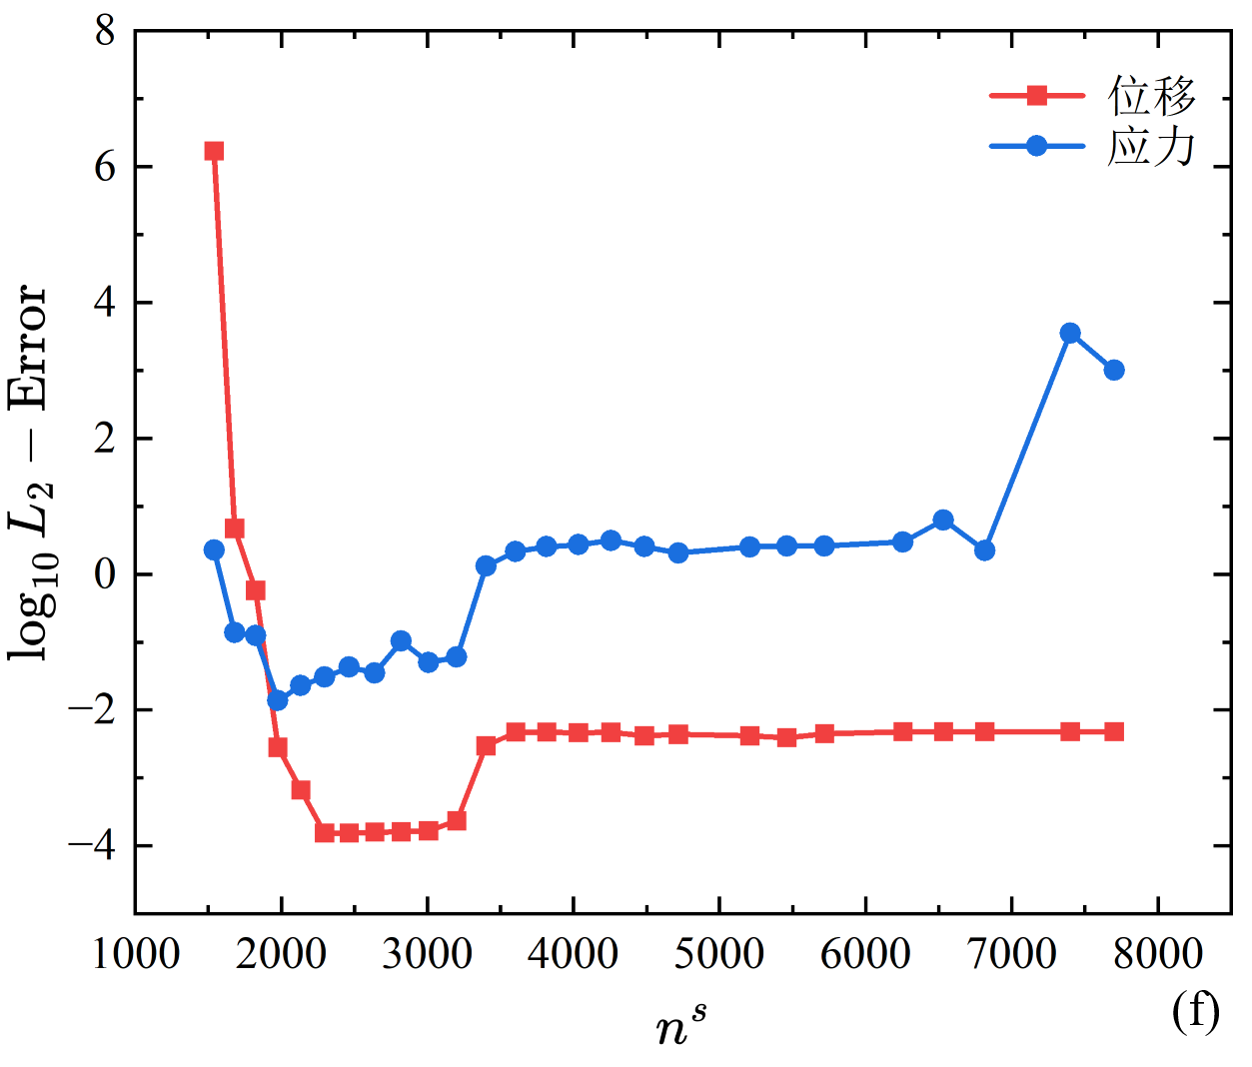
\includegraphics[width=0.49\textwidth]{figures/shearlocking/Q8-l2-ns32.png}
    \phantomcaption\label{Q8-l2-ns32}
    \end{subcaptiongroup}
\caption{\centering{固支方板问题二次单元$L2$误差与剪切应力节点数量的关系:\protect\linebreak 
\subref{T6-l2-ns8},\subref{Q8-l2-ns8} $8\times 8$单元$L_2$误差; 
\subref{T6-l2-ns16},\subref{Q8-l2-ns16} $16\times 16$单元$L_2$误差;
\subref{T6-l2-ns32},\subref{Q8-l2-ns32} $32\times 32$单元$L_2$误差}}
\label{quad-ns}
\end{figure}

分析固支方板问题的应力精确解云图\ref{plate_exact_solution},可以观察到应力$Q\_1$、$Q\_2$具有相似的性质。在进一步的研究中仅针对
$Q\_1$进行探讨。如图\ref{Q1-Tri3}对于Tri3单元,在不同位移节点数量下,传统约束比例与最优约束比例的应力云图存在显著的差异。当节点
数量按照传统约束比例设置时,会出现明显的应力振荡现象。随着位移节点的增加这种应力振荡现象有所的缓解,但仍然存在。相较之下,在最优
约束比下没有发生应力振荡现象。Quad4单元的应力云图\ref{Q1-Quad4}和Quad8单元图\ref{Q1-Quad8}也表现出类似的现象。对于Tri6单元
图\ref{Q1-Tri6}而言,即使位移节点增加,节点数量按照传统约束比设置时,始终会出现应力振荡现象,而最优约束比例时没有发生应力振荡现象。

\begin{figure}[H]
    \centering
    \begin{subcaptiongroup}
    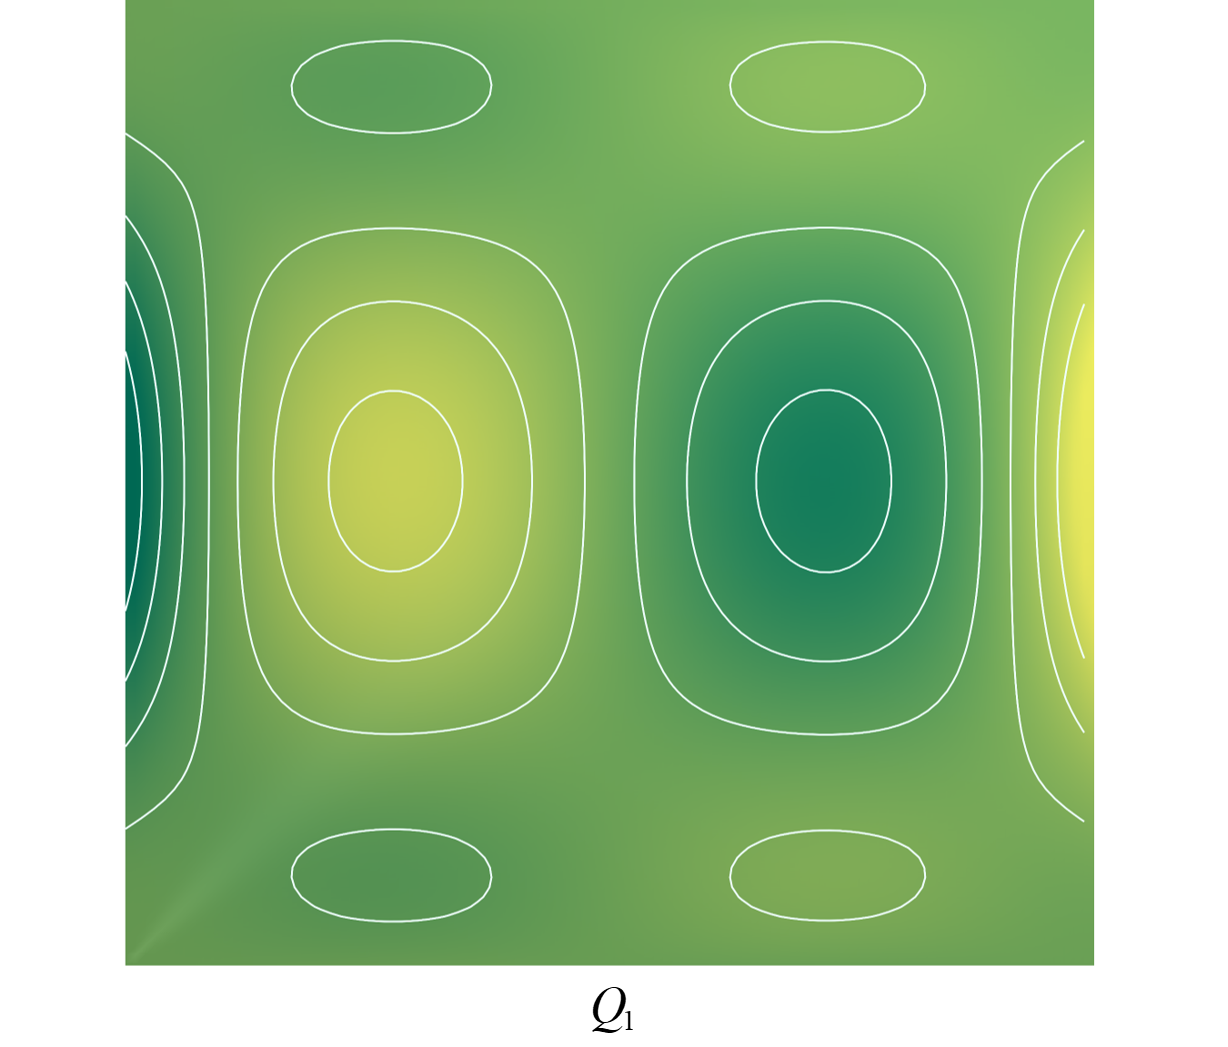
\includegraphics[width=0.46\textwidth]{figures/shearlocking/plate_exactQ1_solution.png}
    \phantomcaption
    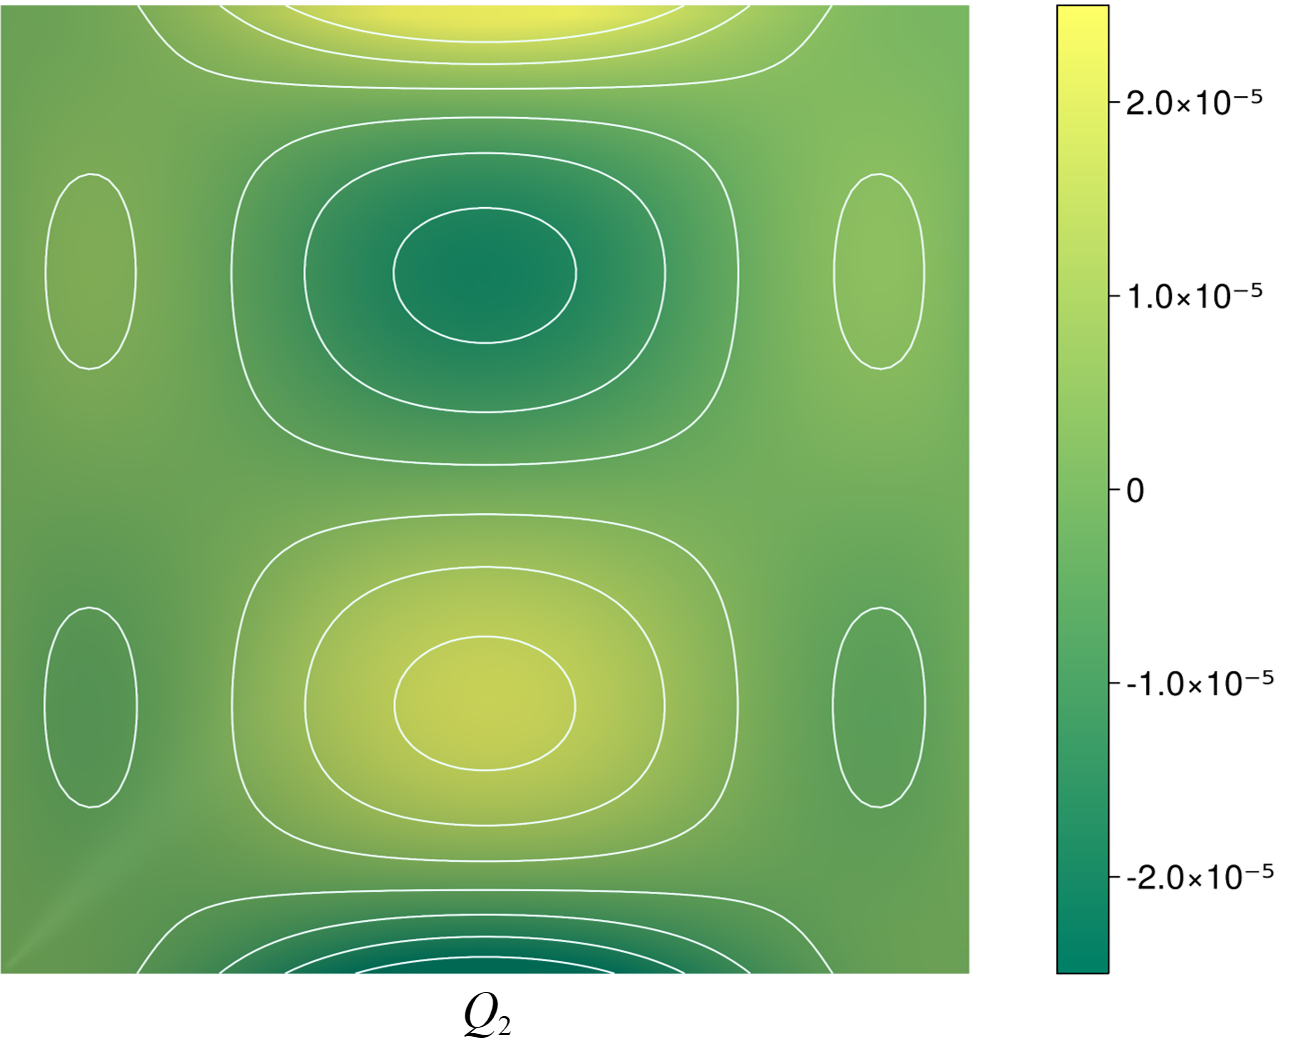
\includegraphics[width=0.49\textwidth]{figures/shearlocking/plate_exactQ2_solution.png}
    \phantomcaption
    \end{subcaptiongroup}
\caption{\centering{固支方板问题应力精确解}}
\label{plate_exact_solution}
\end{figure}

\begin{figure}[H]
    \centering
    \begin{tabular}{cccc}
    $\quad$&最优约束比&传统约束比\\
    $81$&\begin{subcaptiongroup}\raisebox{-0.5\height}{\includegraphics[width=0.4\textwidth]{figures/shearlocking/SquarePlate_T3_q1_8_7.png}}\end{subcaptiongroup}
    &\begin{subcaptiongroup}\raisebox{-0.5\height}{\includegraphics[width=0.4\textwidth]{figures/shearlocking/SquarePlate_T3_q1_8_8.png}}\end{subcaptiongroup}\\
    $289$&\begin{subcaptiongroup}\raisebox{-0.5\height}{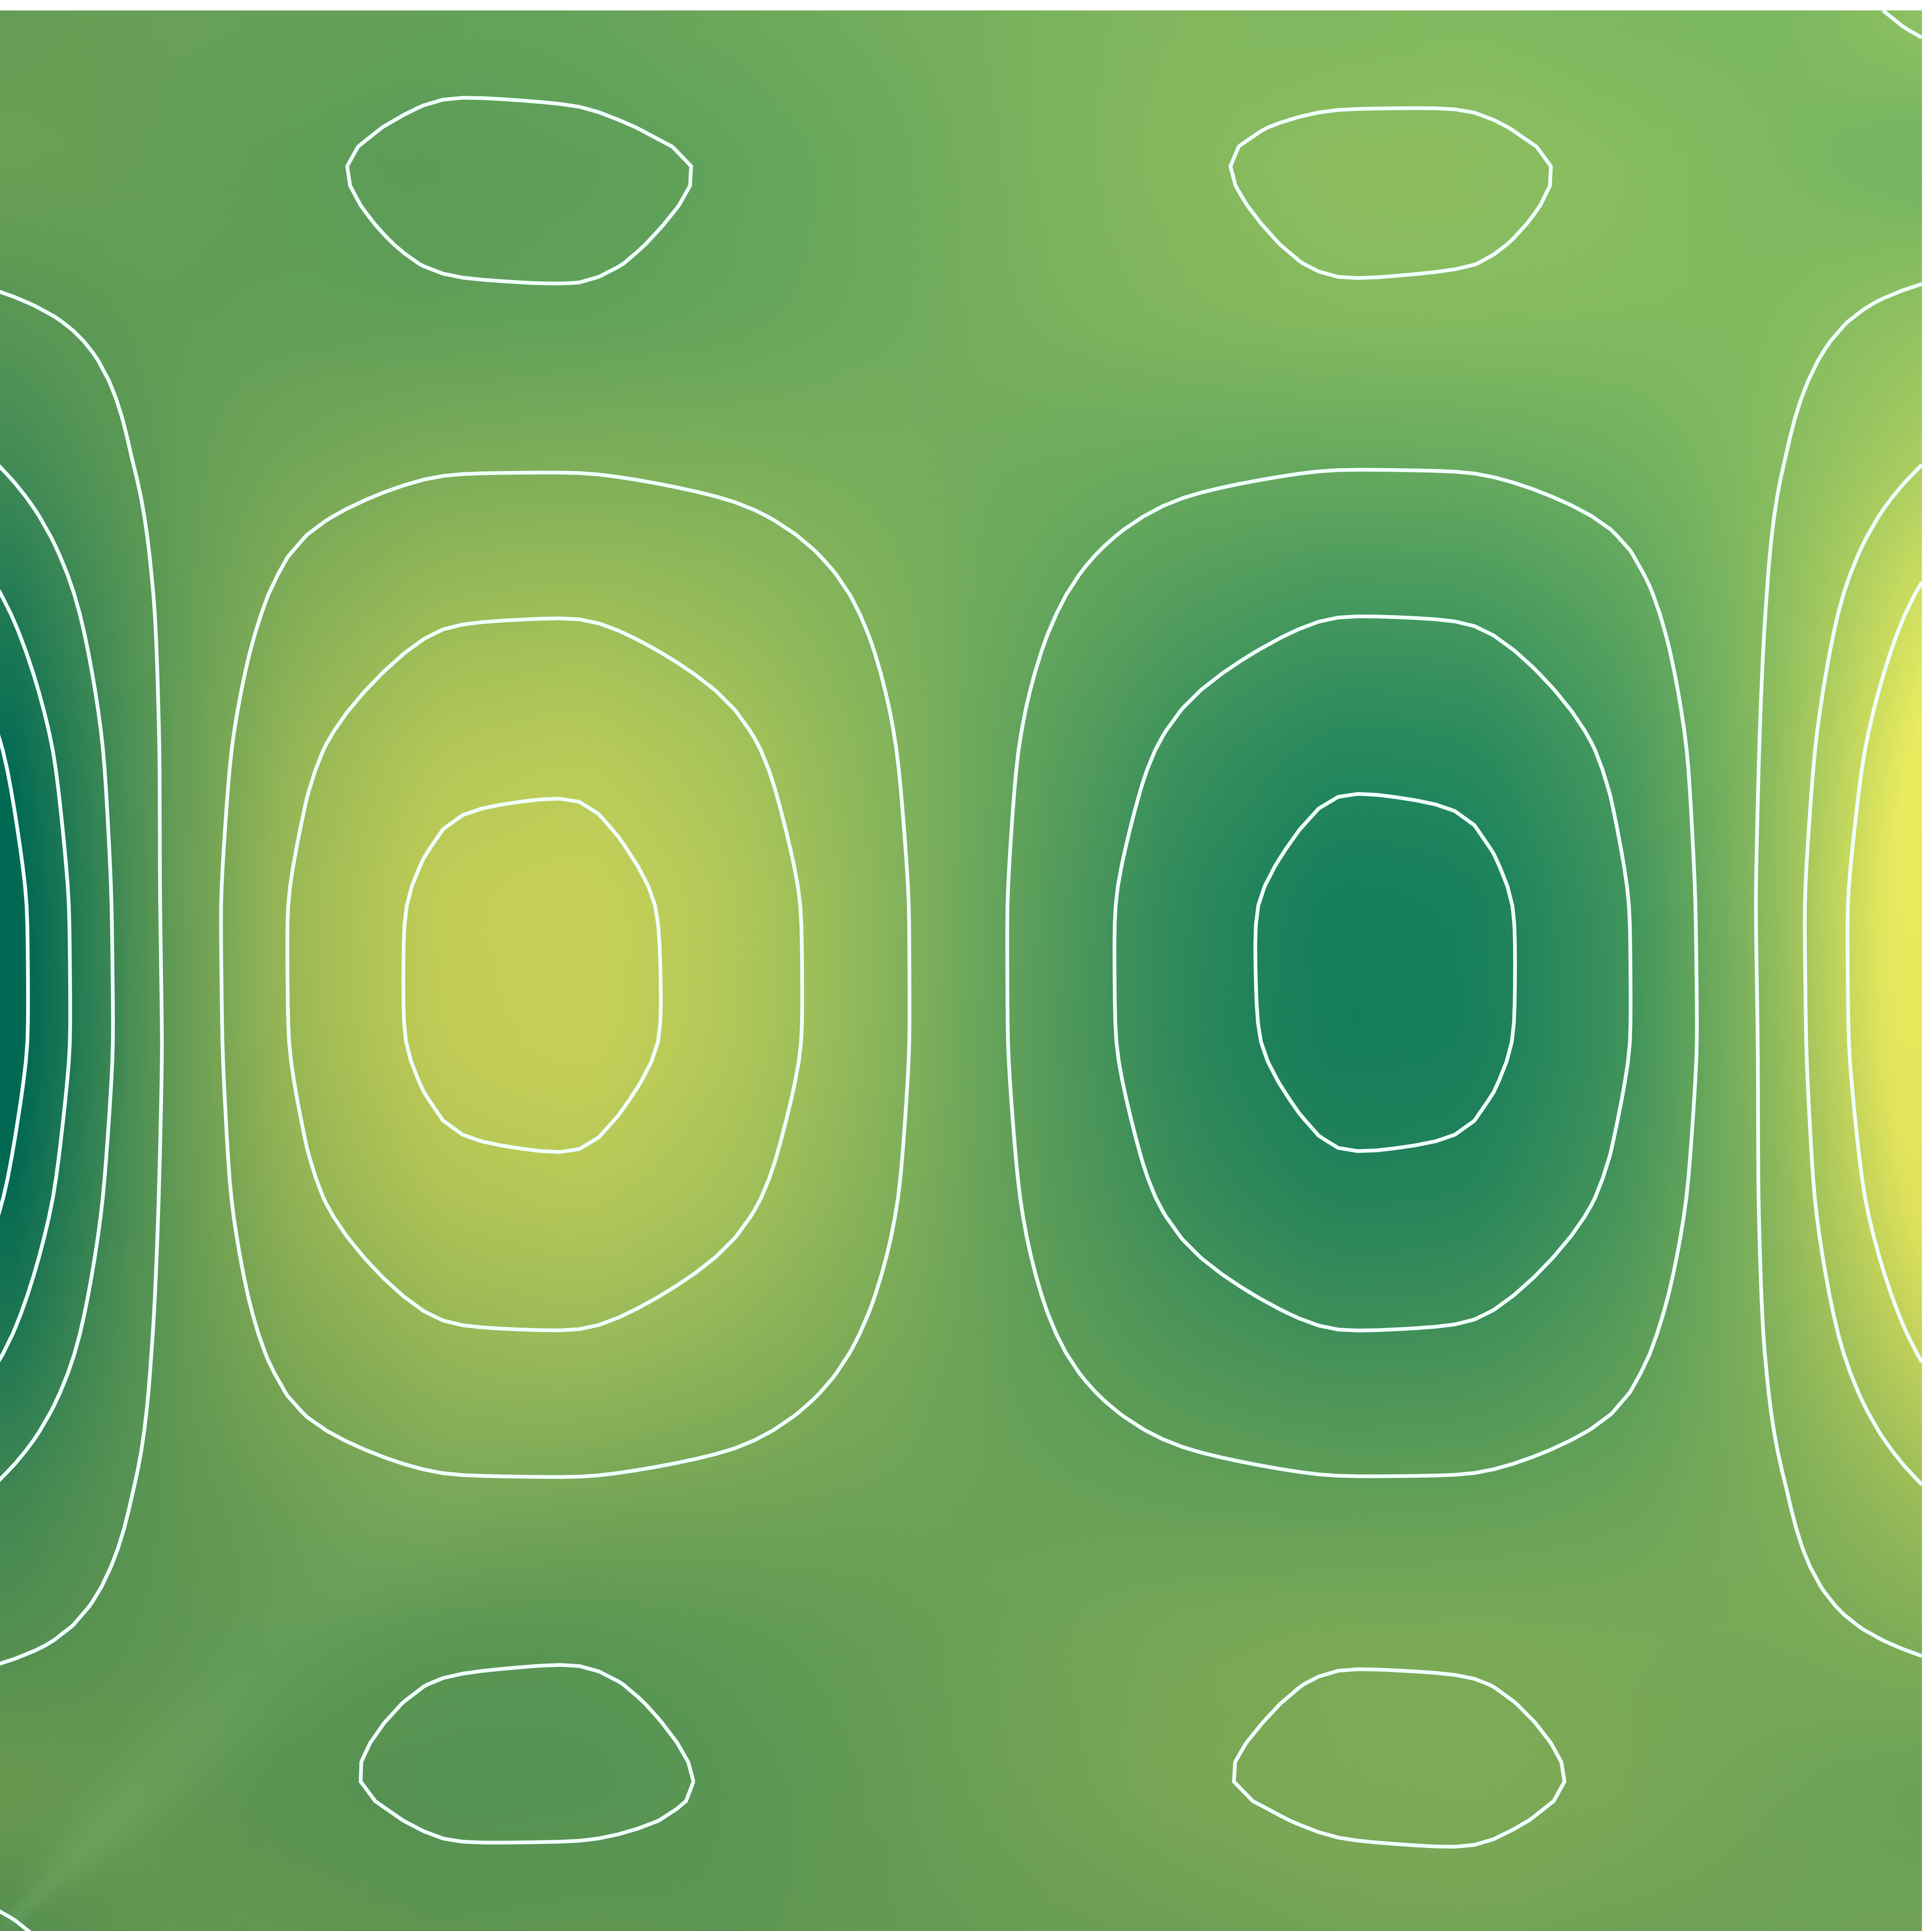
\includegraphics[width=0.4\textwidth]{figures/shearlocking/SquarePlate_T3_q1_16_13.png}}\end{subcaptiongroup}
    &\begin{subcaptiongroup}\raisebox{-0.5\height}{\includegraphics[width=0.4\textwidth]{figures/shearlocking/SquarePlate_T3_q1_16_16.png}}\end{subcaptiongroup}\\
    $1089$&\begin{subcaptiongroup}\raisebox{-0.5\height}{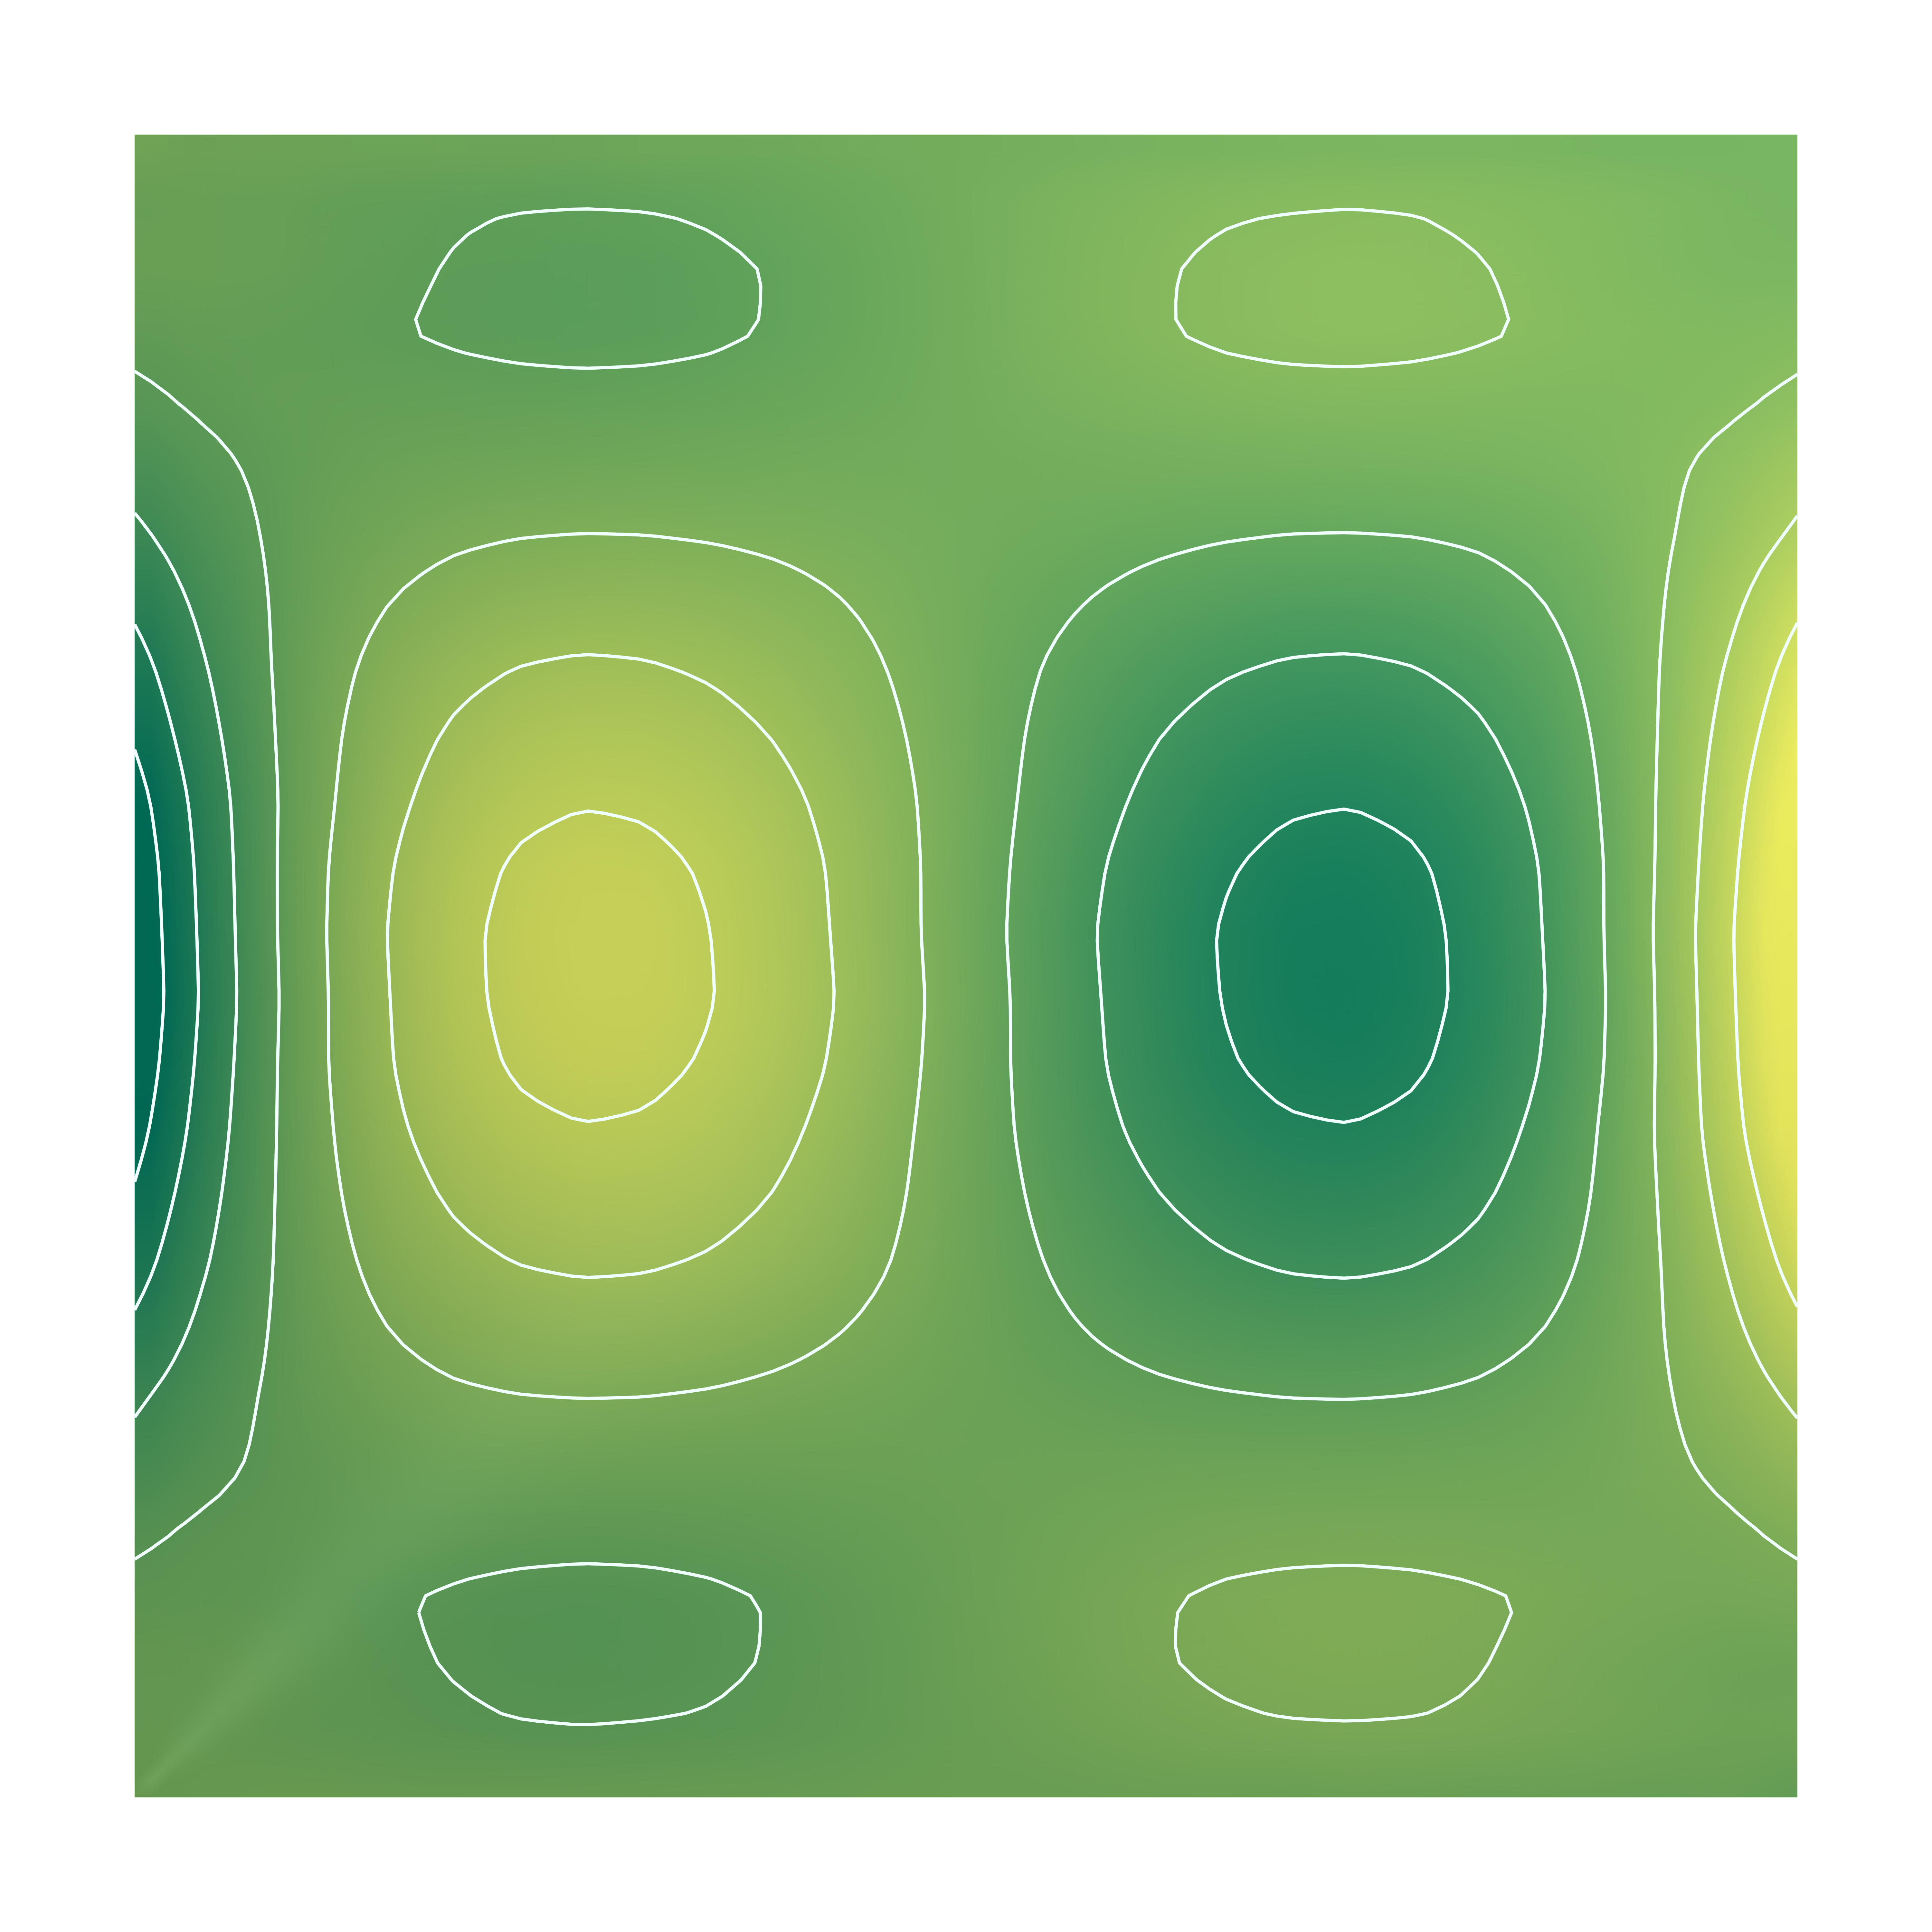
\includegraphics[width=0.4\textwidth]{figures/shearlocking/SquarePlate_T3_q1_32_26.png}}\end{subcaptiongroup}
    &\begin{subcaptiongroup}\raisebox{-0.5\height}{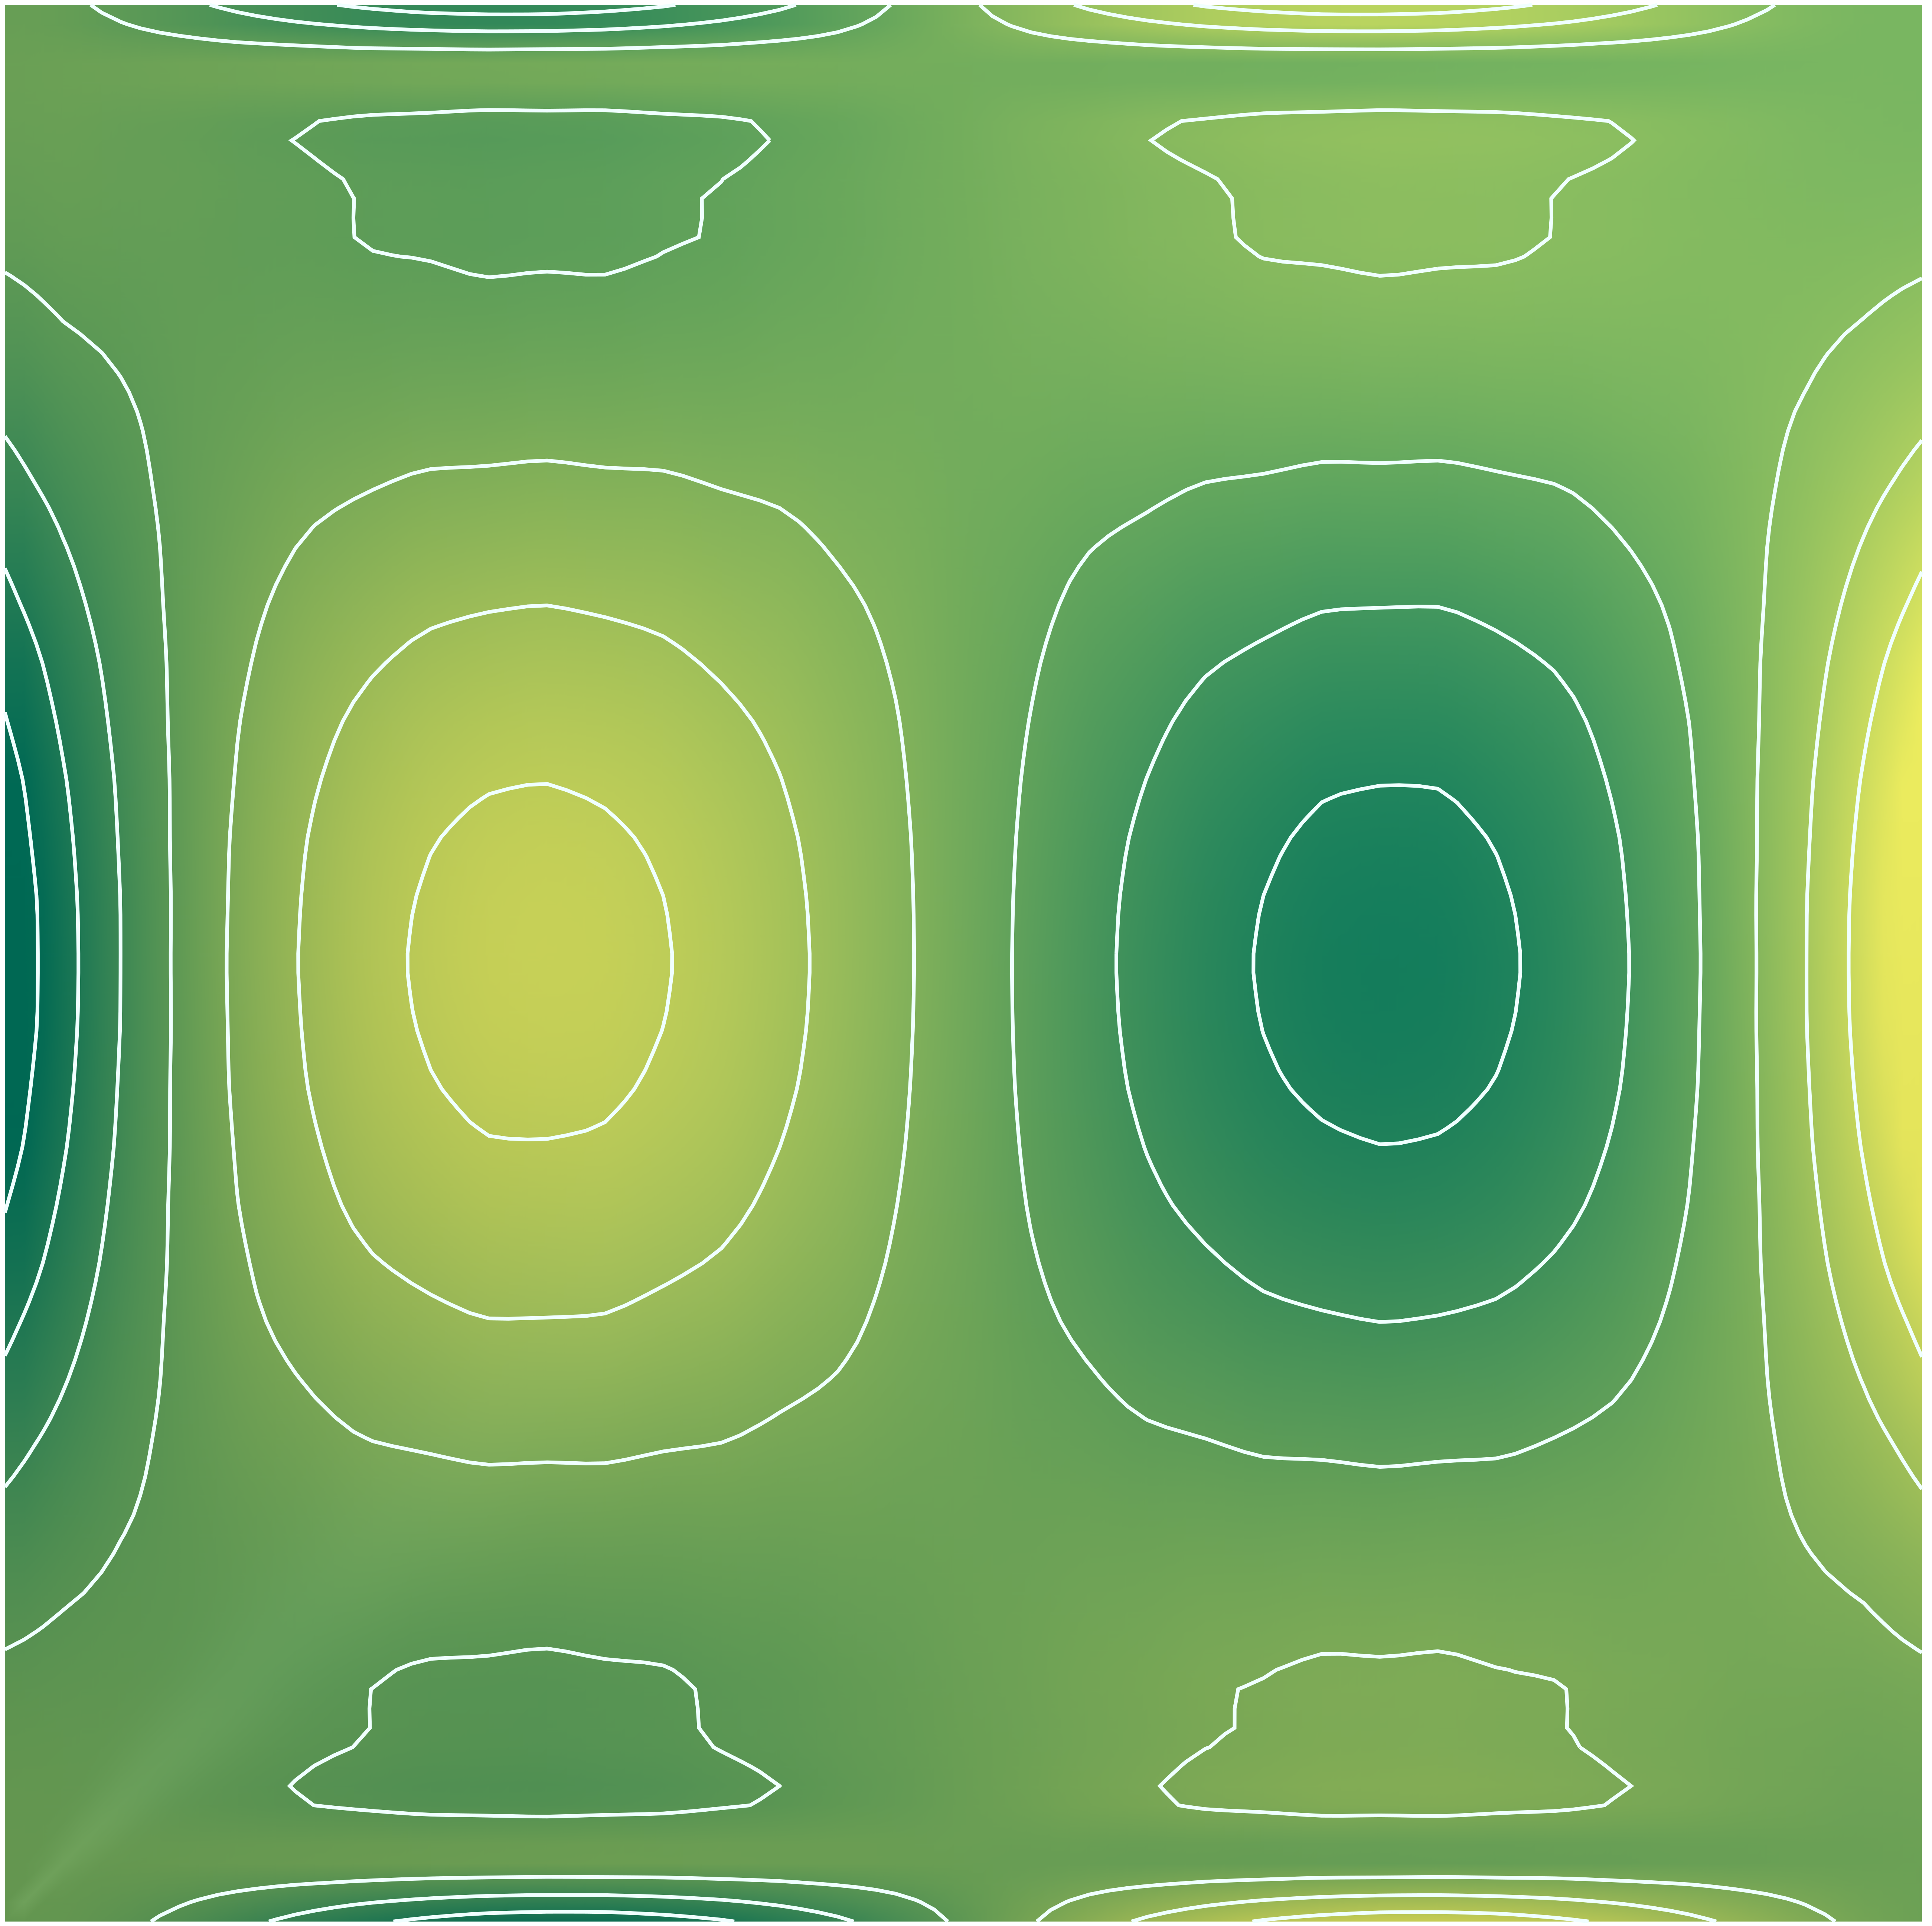
\includegraphics[width=0.4\textwidth]{figures/shearlocking/SquarePlate_T3_q1_32_32.png}}\end{subcaptiongroup}\\
    \end{tabular}
    \caption{\textbf{Tri3单元应力云图($Q_1$)}}\label{Q1-Tri3}
\end{figure}

\begin{figure}[H]
    \centering
    \begin{tabular}{cccc}
    $\quad$&最优约束比&传统约束比\\
    $81$&\begin{subcaptiongroup}\raisebox{-0.5\height}{\includegraphics[width=0.4\textwidth]{figures/shearlocking/SquarePlate_mix_quad4_q1_8_7.png}}\end{subcaptiongroup}
    &\begin{subcaptiongroup}\raisebox{-0.5\height}{\includegraphics[width=0.4\textwidth]{figures/shearlocking/SquarePlate_mix_quad4_q1_8_8.png}}\end{subcaptiongroup}\\
    $289$&\begin{subcaptiongroup}\raisebox{-0.5\height}{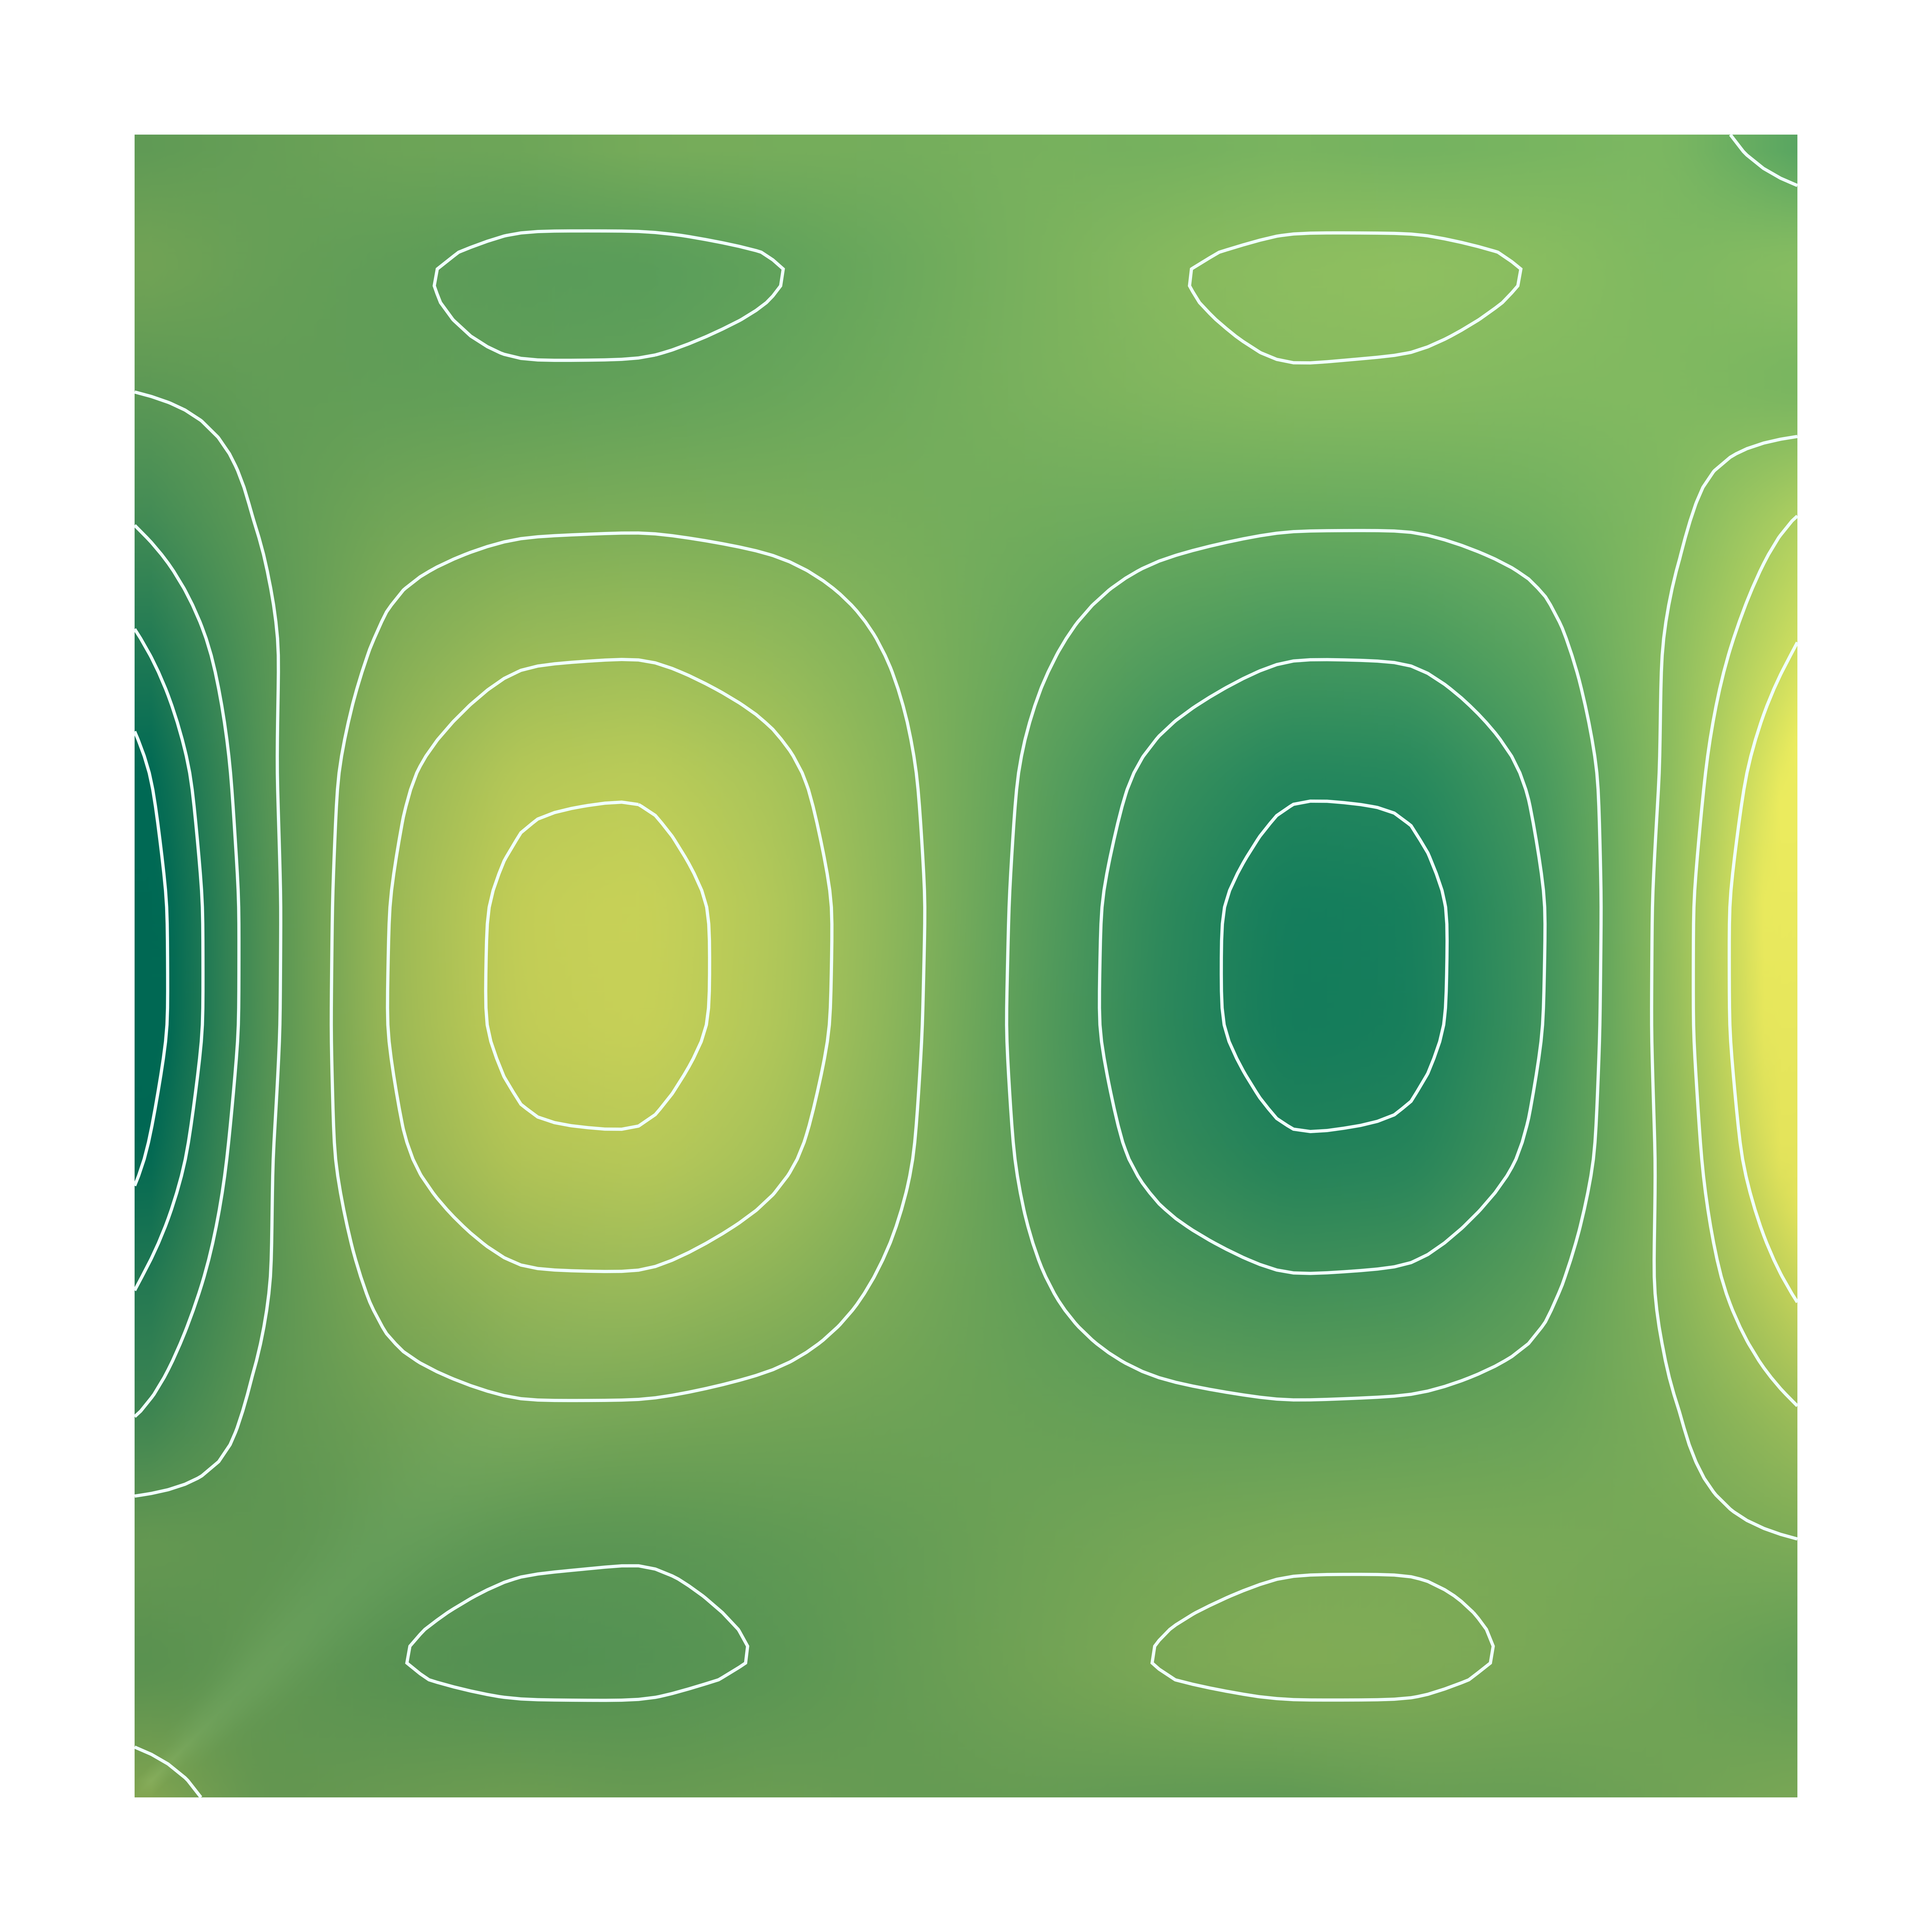
\includegraphics[width=0.4\textwidth]{figures/shearlocking/SquarePlate_mix_quad4_q1_16_13.png}}\end{subcaptiongroup}
    &\begin{subcaptiongroup}\raisebox{-0.5\height}{\includegraphics[width=0.4\textwidth]{figures/shearlocking/SquarePlate_mix_quad4_q1_16_16.png}}\end{subcaptiongroup}\\
    $1089$&\begin{subcaptiongroup}\raisebox{-0.5\height}{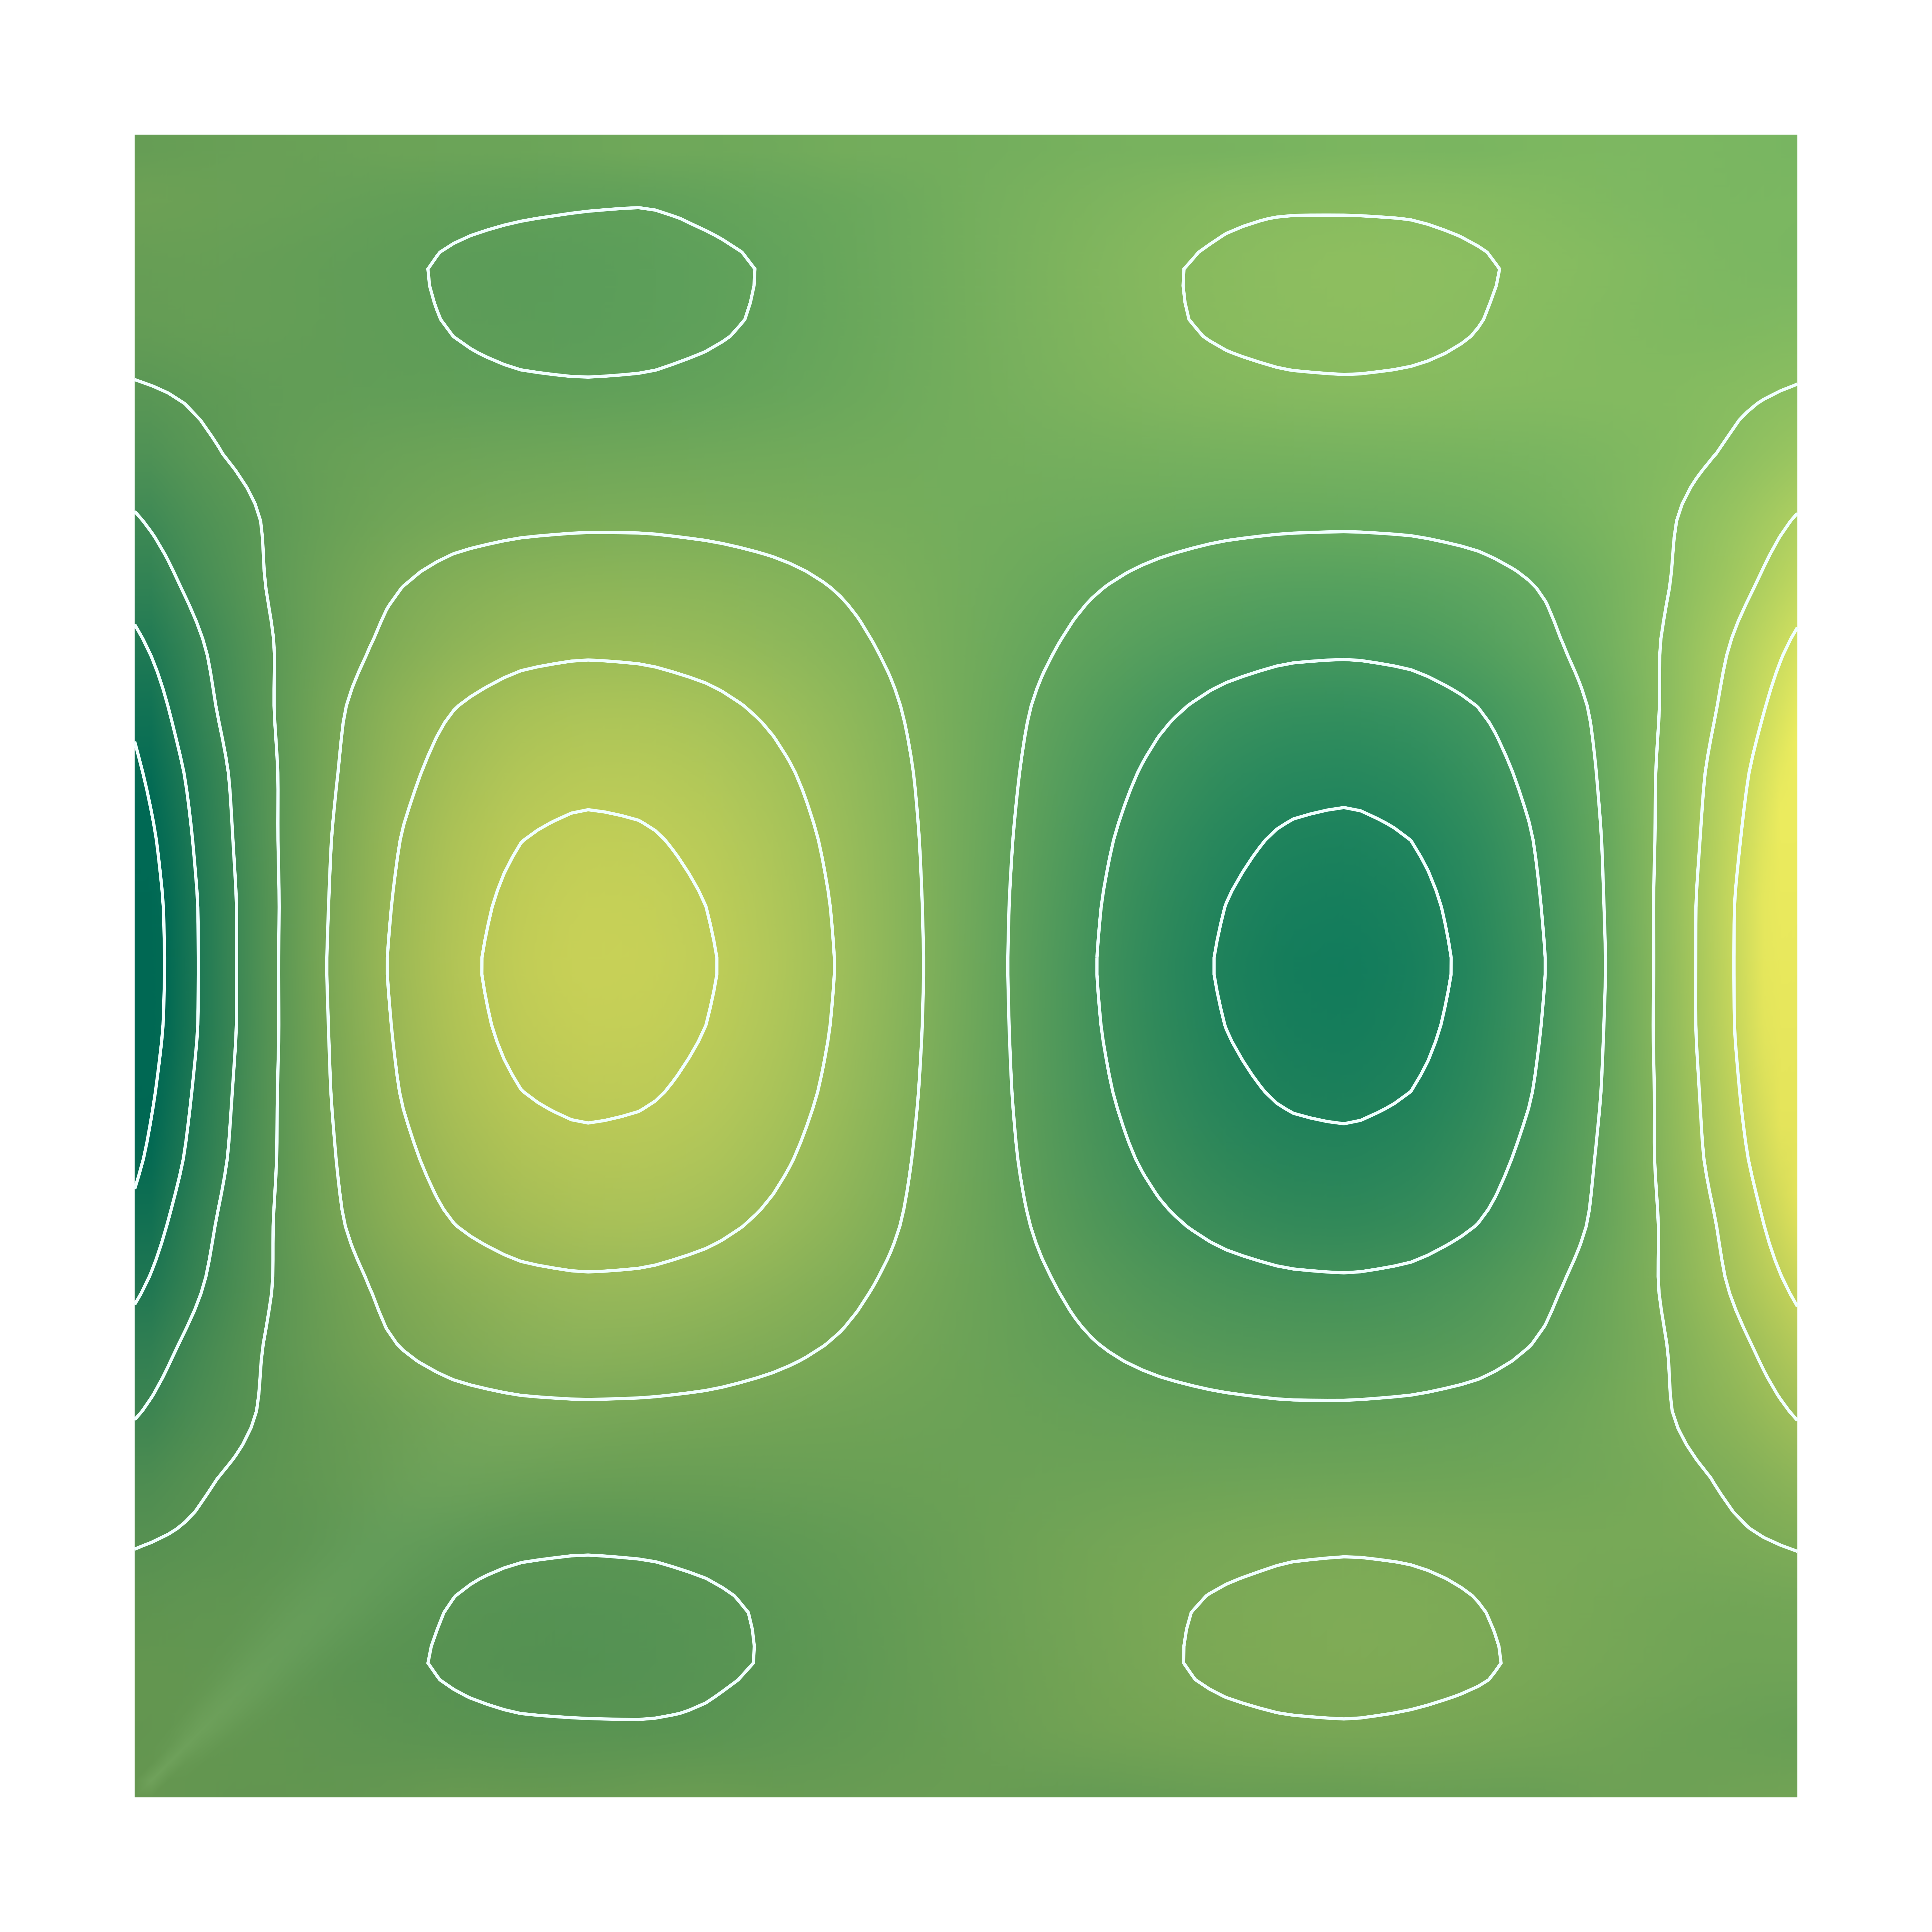
\includegraphics[width=0.4\textwidth]{figures/shearlocking/SquarePlate_mix_quad4_q1_32_26.png}}\end{subcaptiongroup}
    &\begin{subcaptiongroup}\raisebox{-0.5\height}{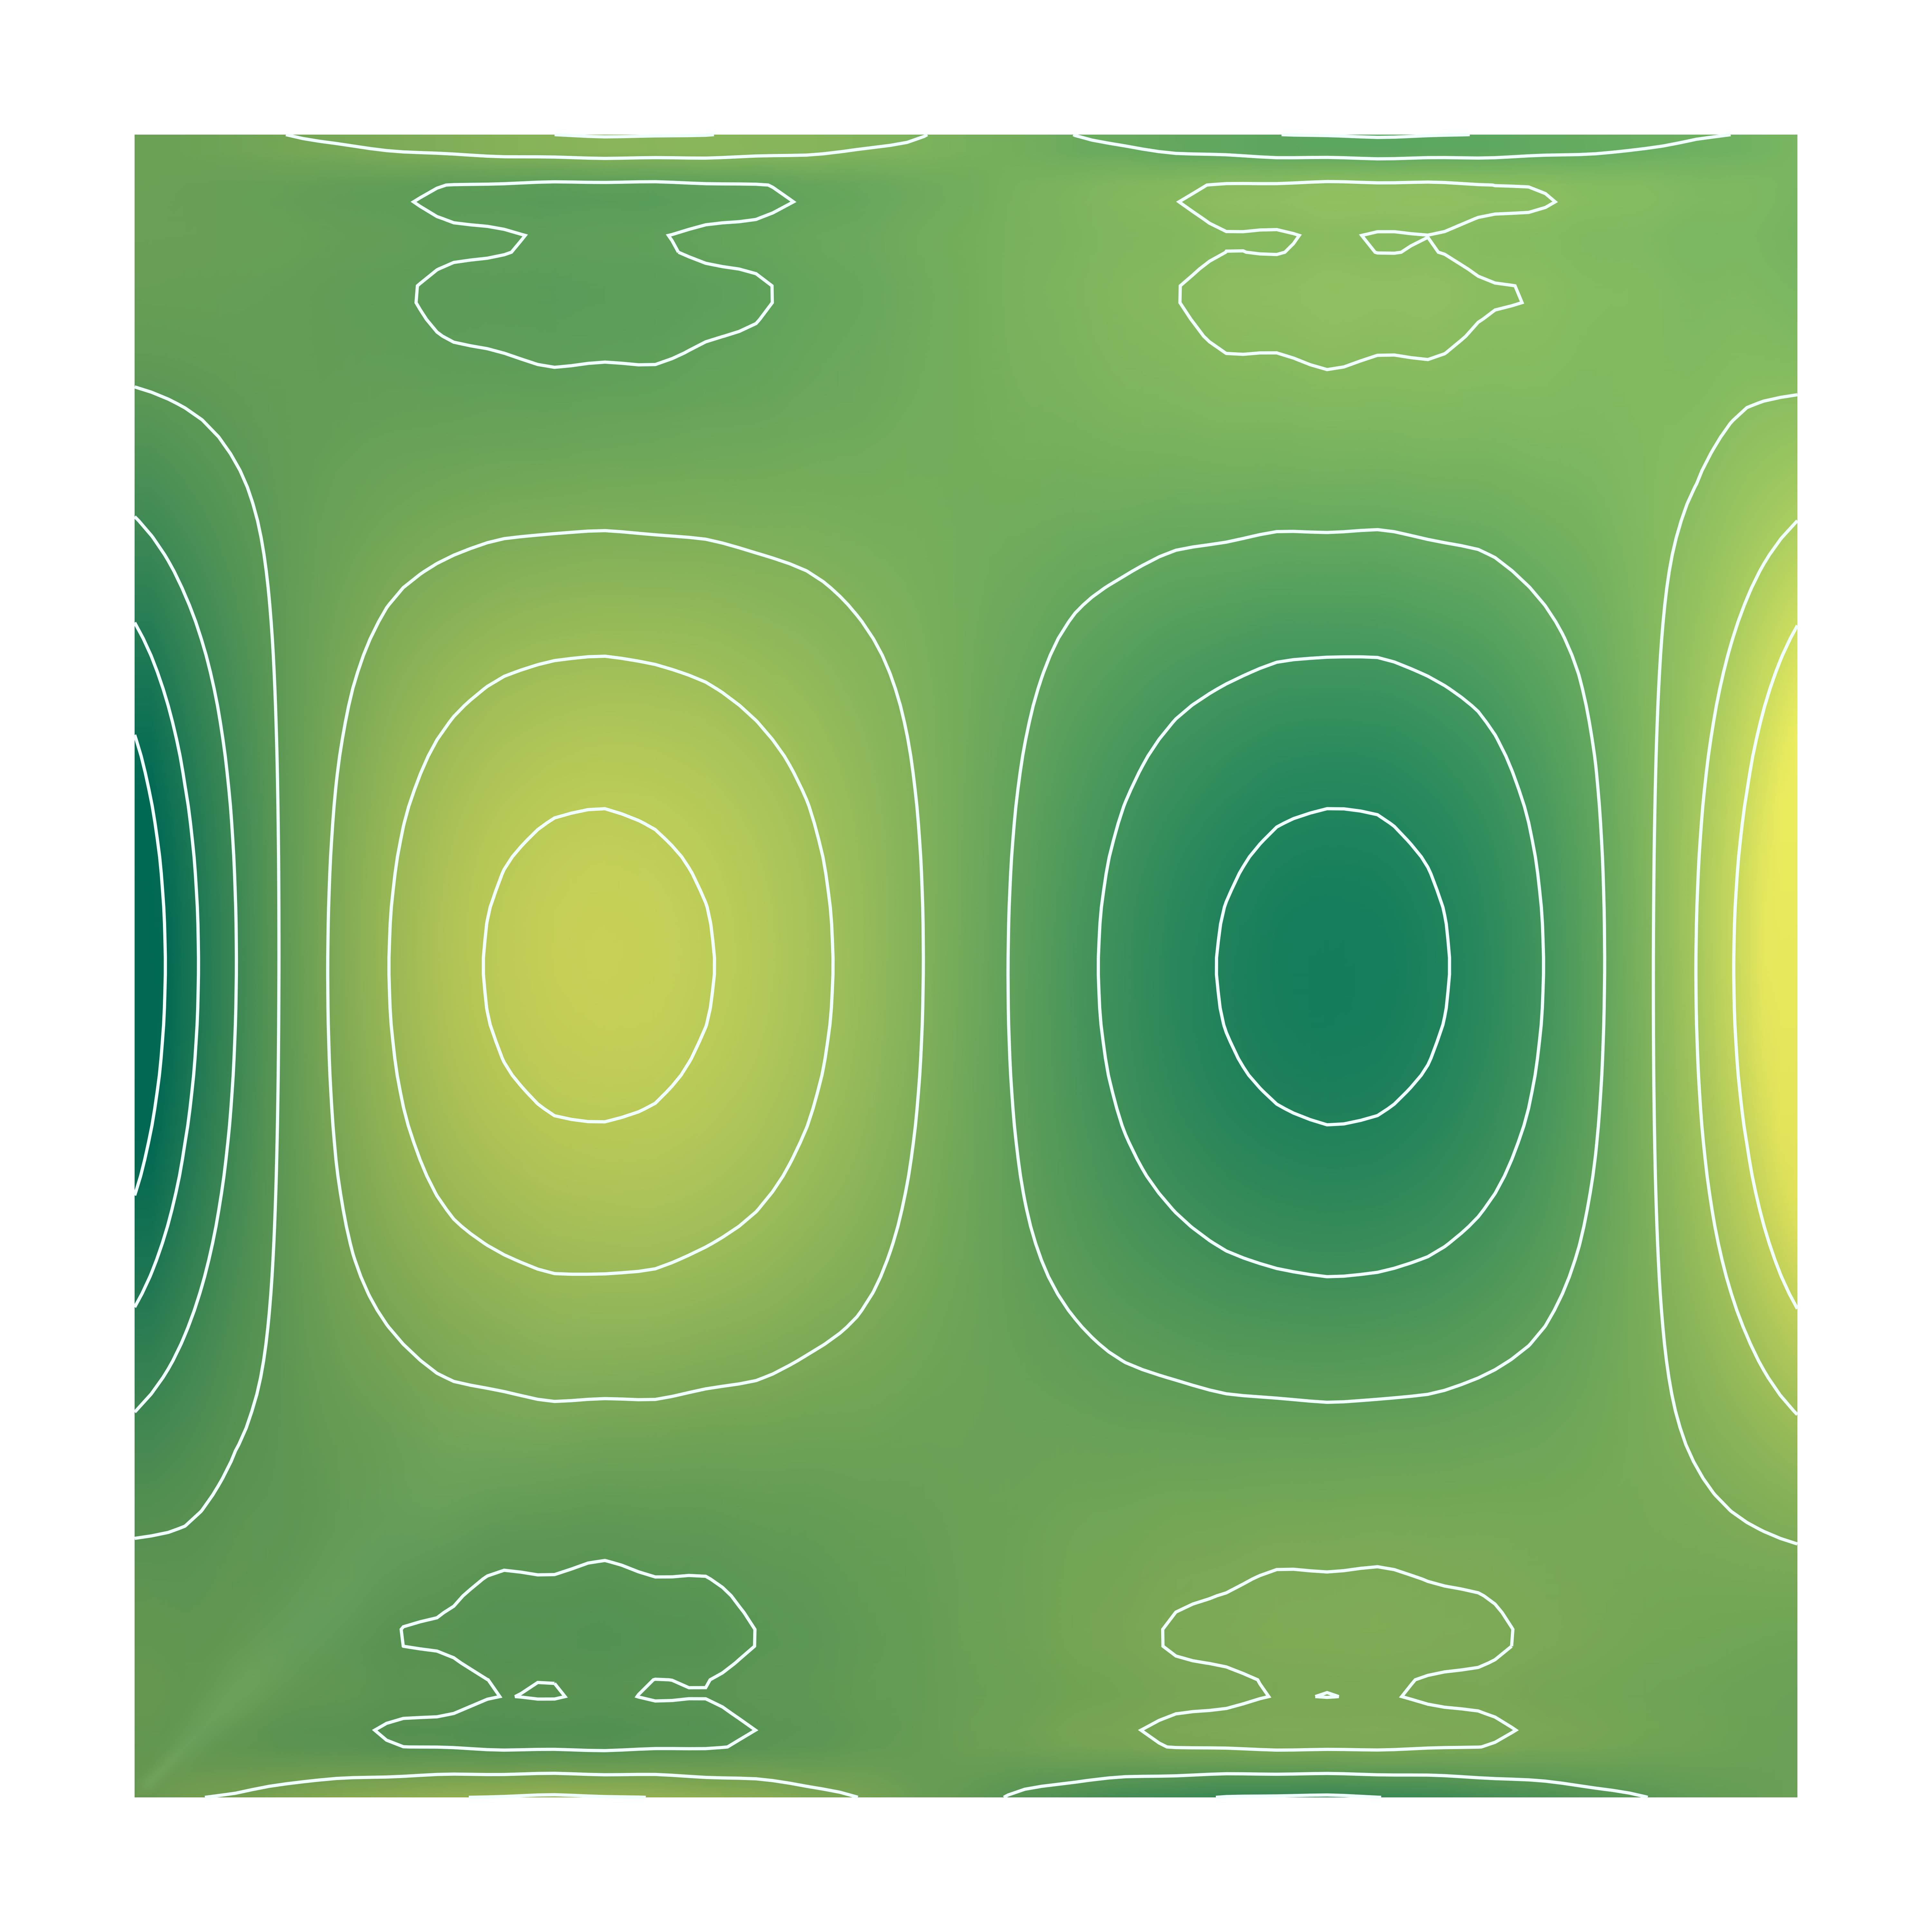
\includegraphics[width=0.4\textwidth]{figures/shearlocking/SquarePlate_mix_quad4_q1_32_32.png}}\end{subcaptiongroup}\\
    \end{tabular}
    \caption{\textbf{Quad4单元应力云图($Q_1$)}}\label{Q1-Quad4}
\end{figure}

\begin{figure}[H]
    \centering
    \begin{tabular}{cccc}
    $\quad$&最优约束比&传统约束比\\
    $289$&\begin{subcaptiongroup}\raisebox{-0.5\height}{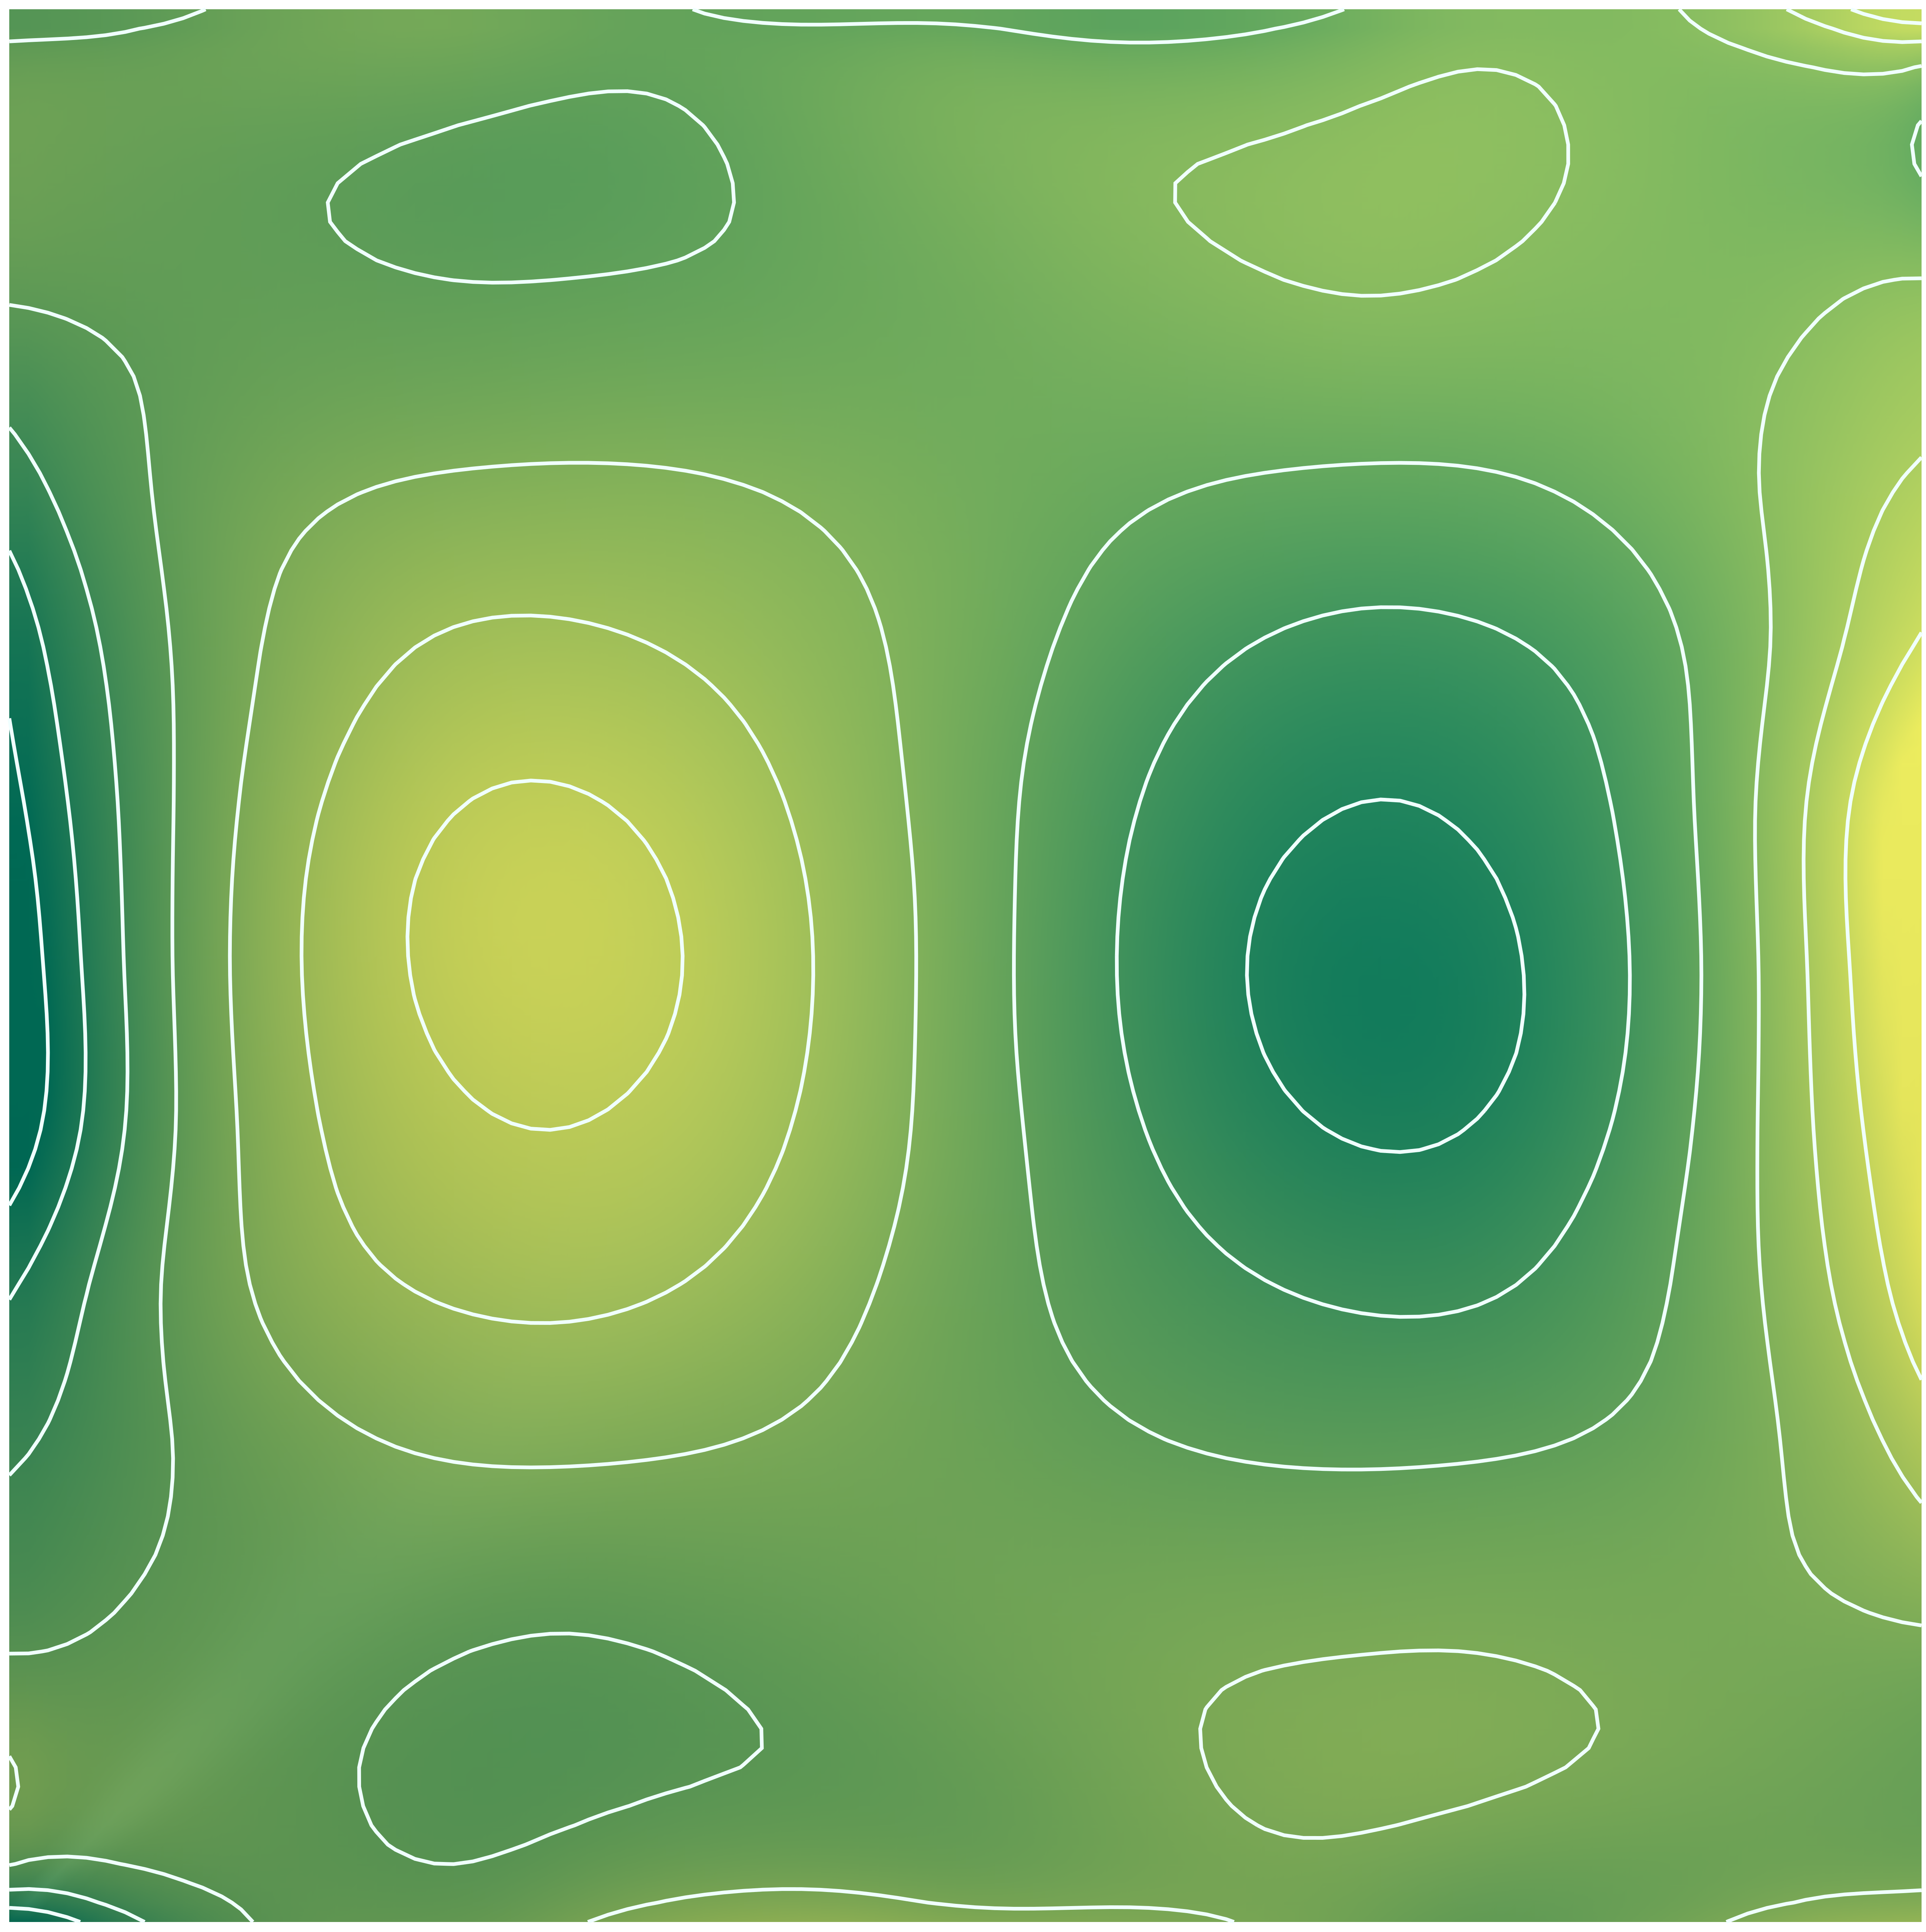
\includegraphics[width=0.4\textwidth]{figures/shearlocking/SquarePlate_mix_tri6_q1_8_6.png}}\end{subcaptiongroup}
    &\begin{subcaptiongroup}\raisebox{-0.5\height}{\includegraphics[width=0.4\textwidth]{figures/shearlocking/SquarePlate_mix_tri6_q1_8_8.png}}\end{subcaptiongroup}\\
    $1089$&\begin{subcaptiongroup}\raisebox{-0.5\height}{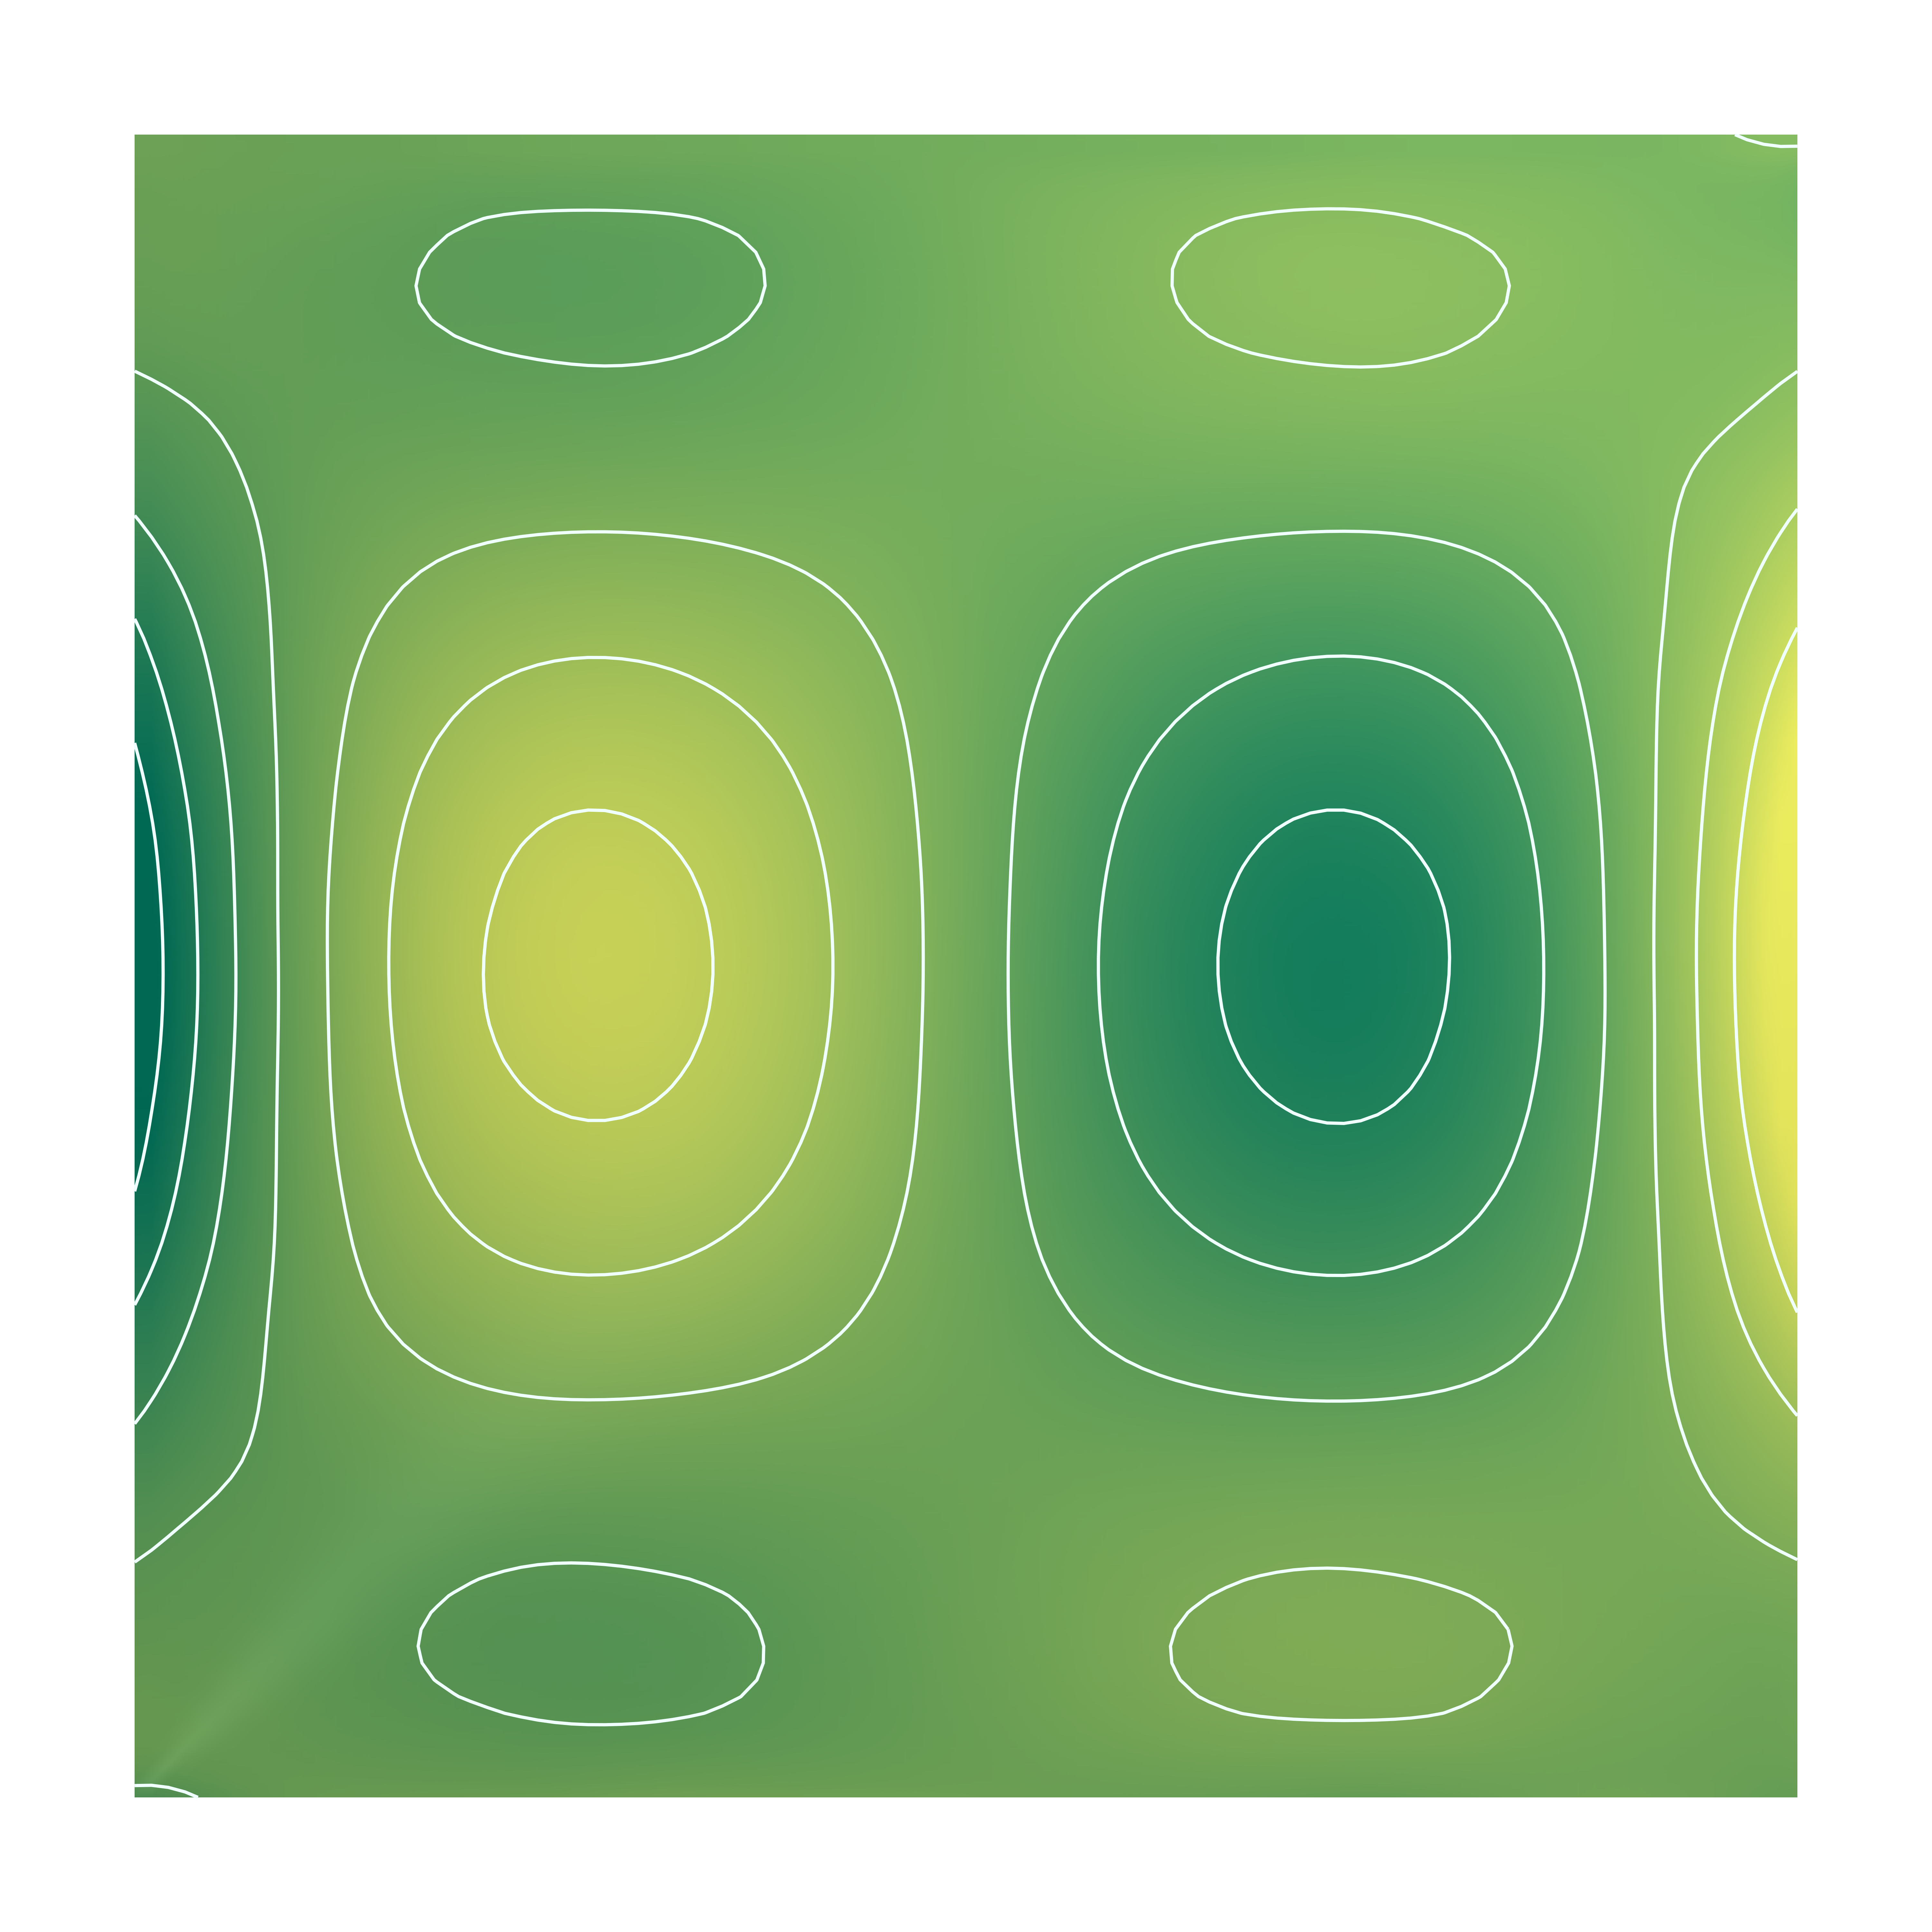
\includegraphics[width=0.4\textwidth]{figures/shearlocking/SquarePlate_mix_tri6_q1_16_12.png}}\end{subcaptiongroup}
    &\begin{subcaptiongroup}\raisebox{-0.5\height}{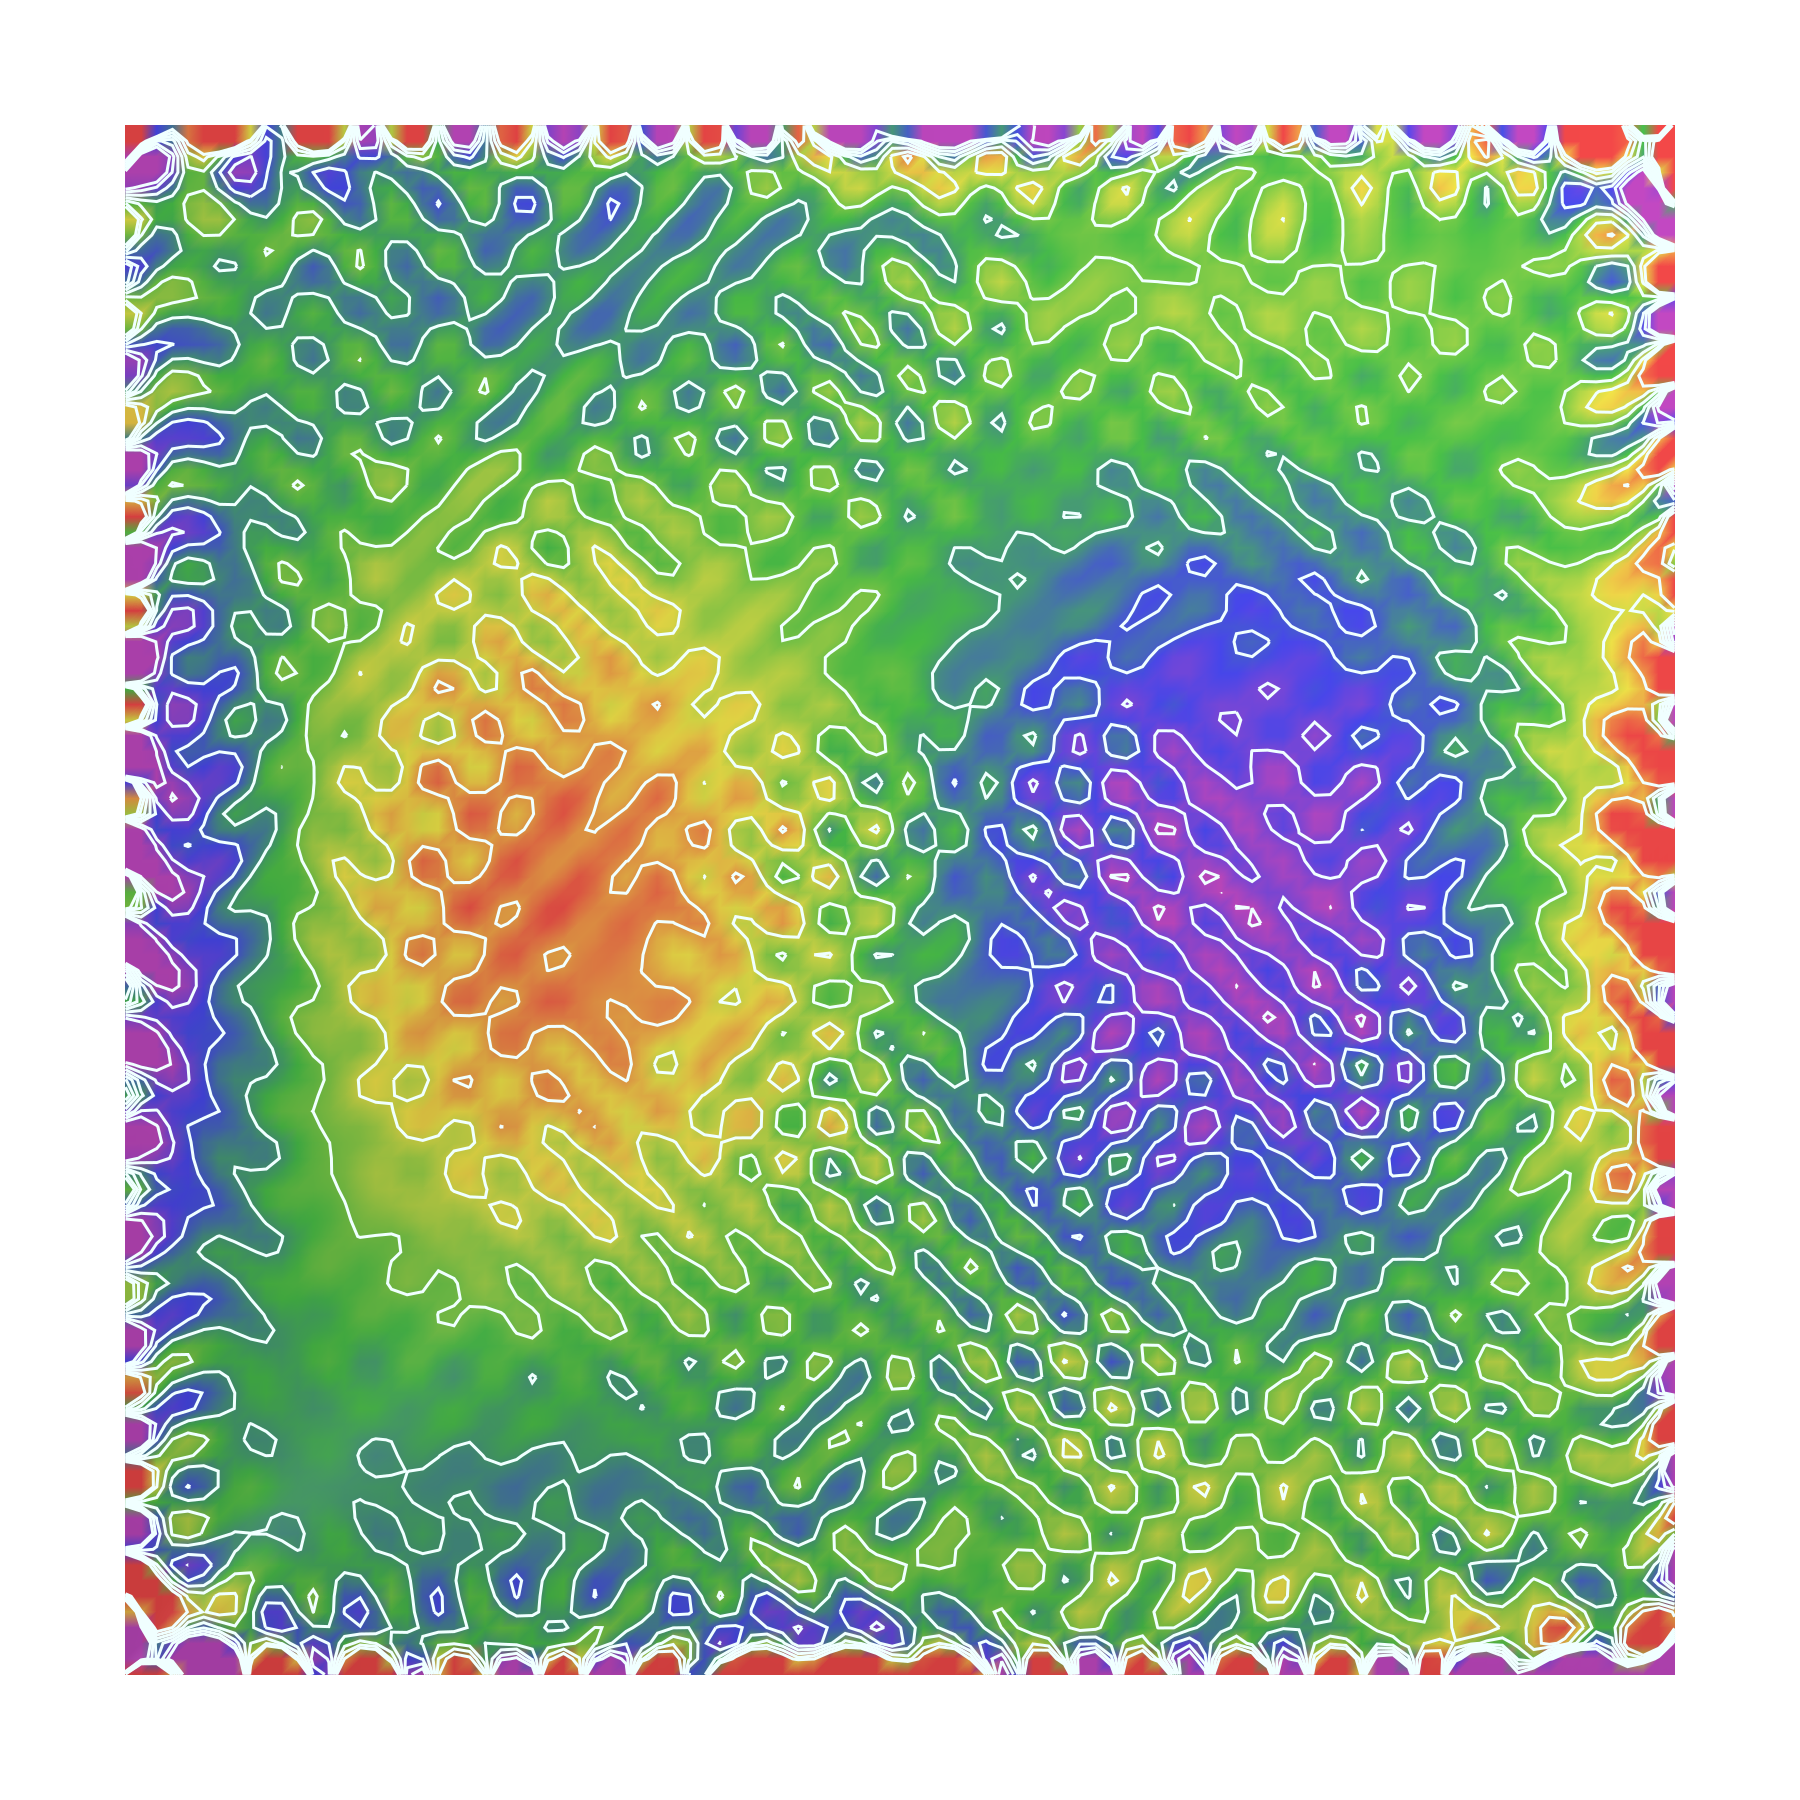
\includegraphics[width=0.4\textwidth]{figures/shearlocking/SquarePlate_mix_tri6_q1_16_16.png}}\end{subcaptiongroup}\\
    $4225$&\begin{subcaptiongroup}\raisebox{-0.5\height}{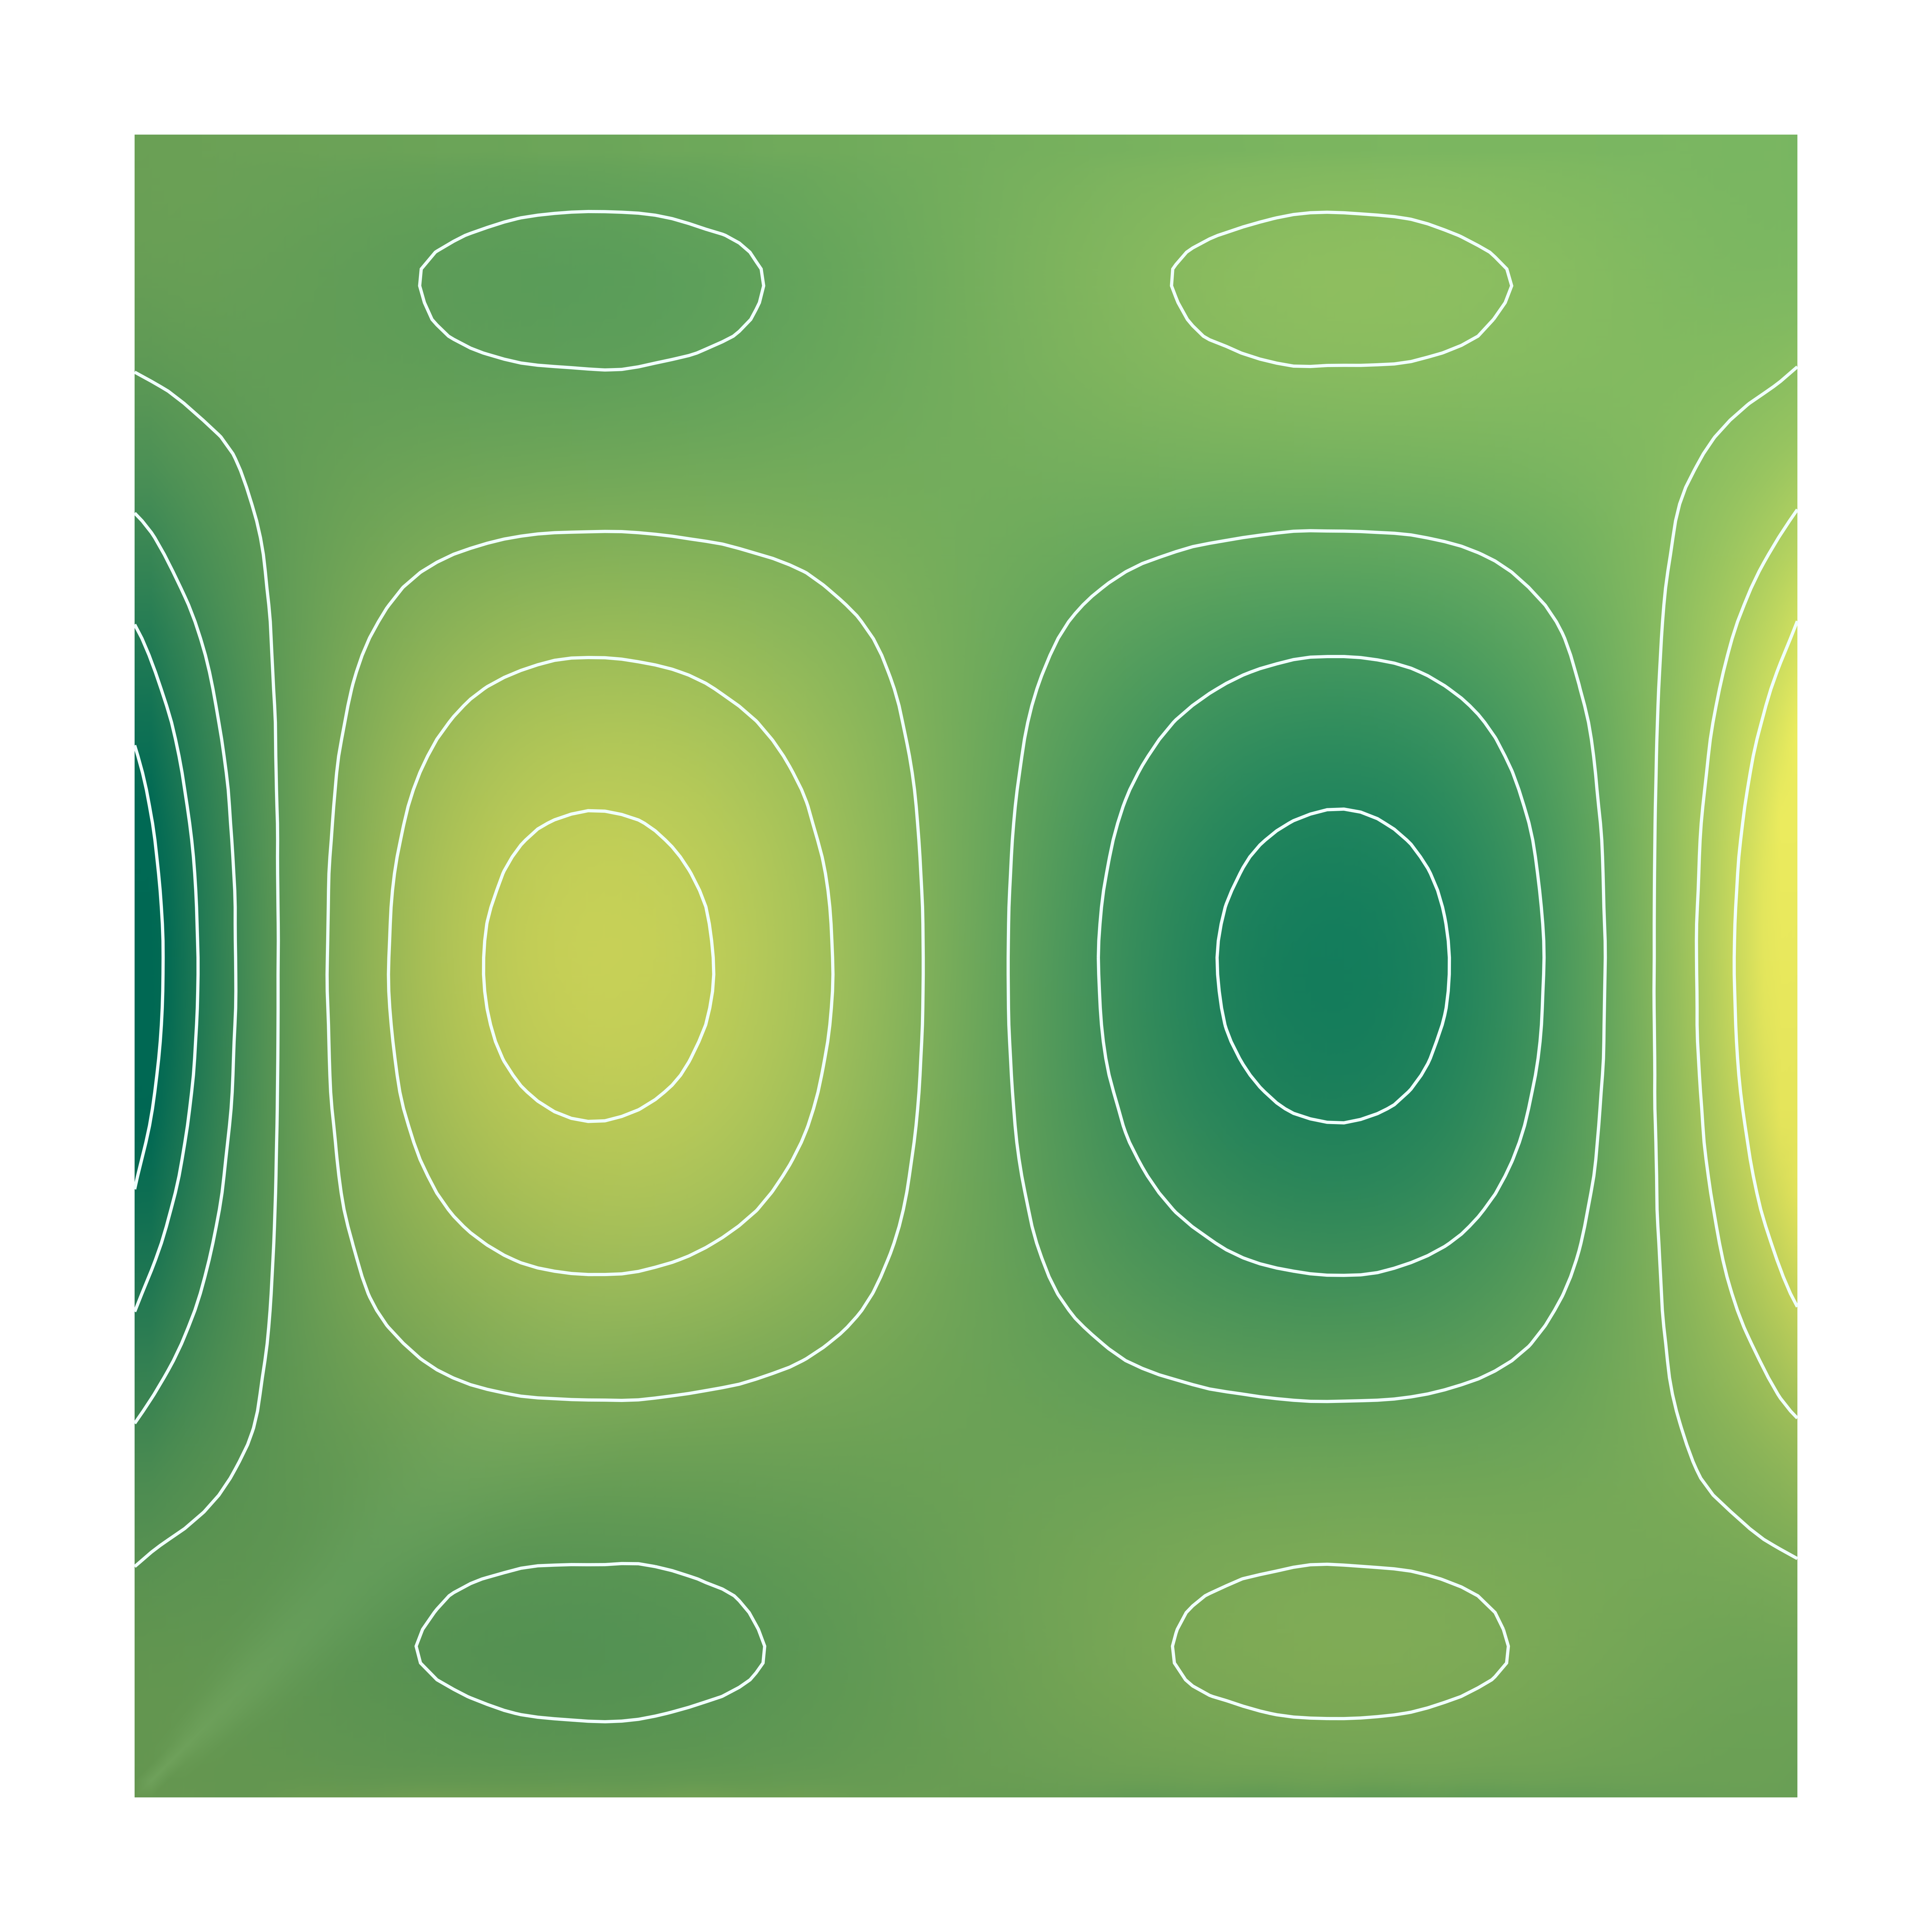
\includegraphics[width=0.4\textwidth]{figures/shearlocking/SquarePlate_mix_tri6_q1_32_25.png}}\end{subcaptiongroup}
    &\begin{subcaptiongroup}\raisebox{-0.5\height}{\includegraphics[width=0.4\textwidth]{figures/shearlocking/SquarePlate_mix_tri6_q1_32_32.png}}\end{subcaptiongroup}\\  
    \end{tabular}
    \caption{\textbf{Tri6单元应力云图($Q_1$)}}\label{Q1-Tri6}
\end{figure}

\begin{figure}[H]
    \centering
    \begin{tabular}{cccc}
    $\quad$&最优约束比&传统约束比\\
    $225$&\begin{subcaptiongroup}\raisebox{-0.4\height}{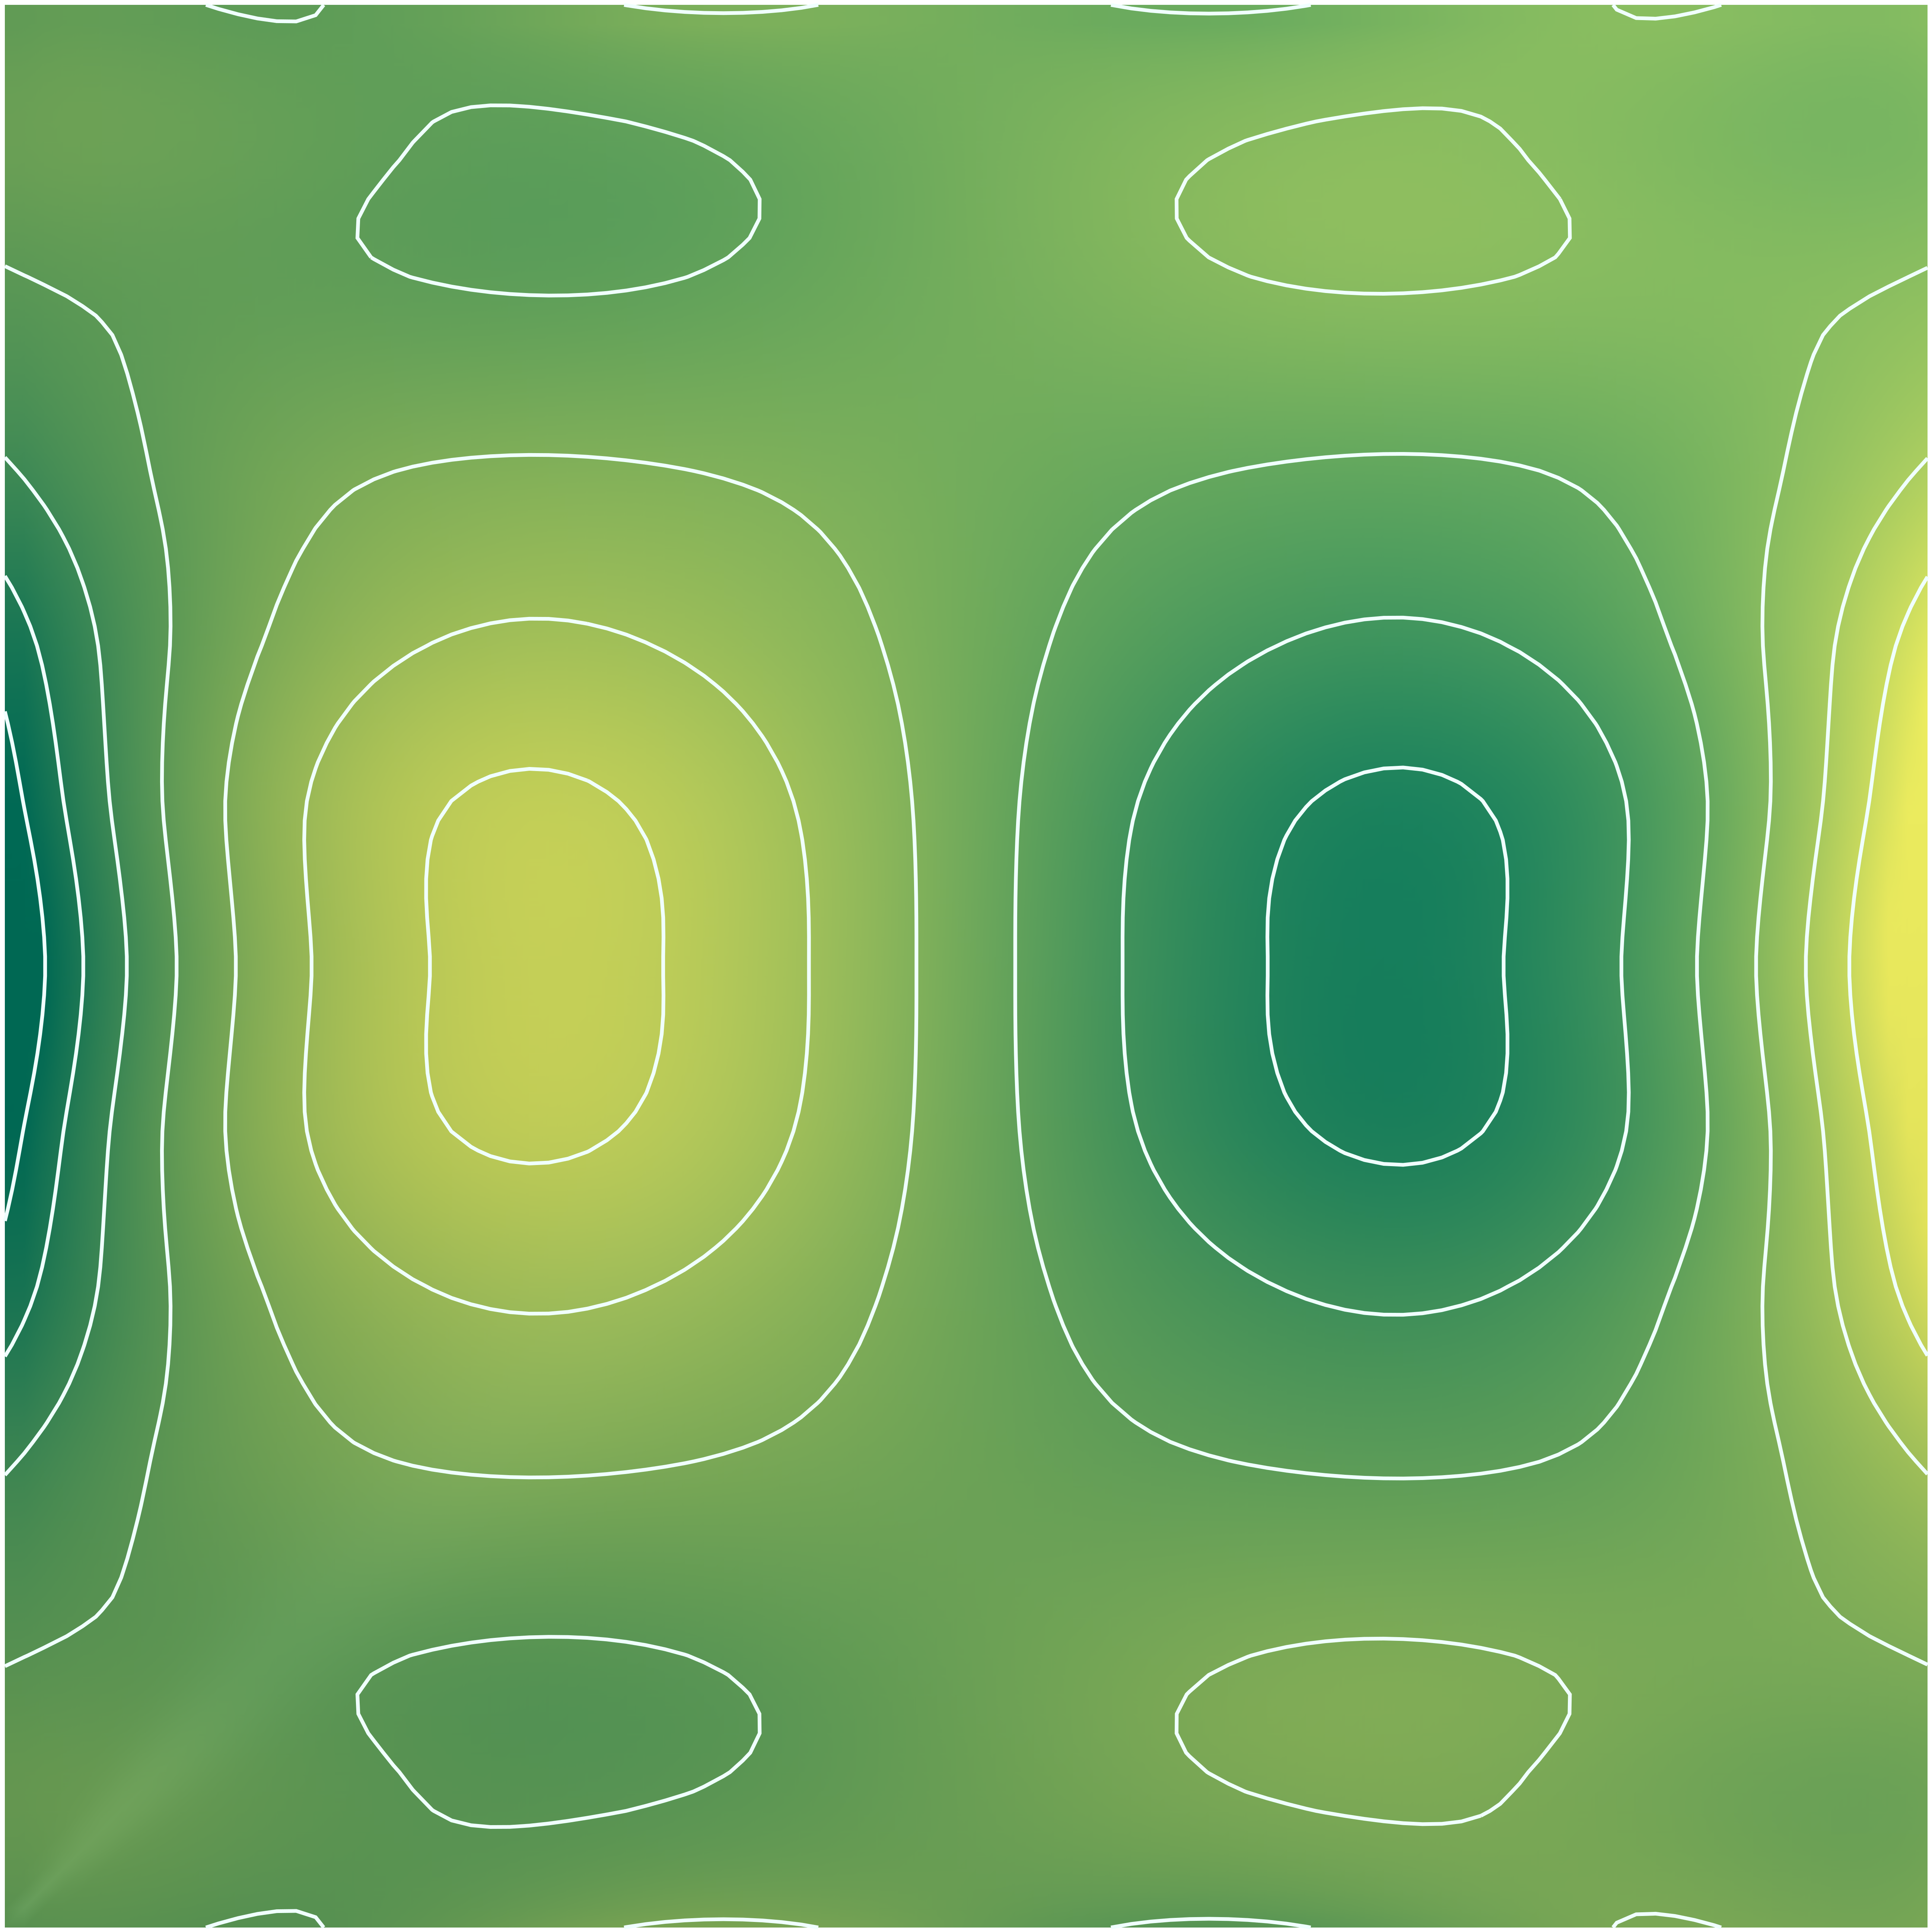
\includegraphics[width=0.4\textwidth]{figures/shearlocking/SquarePlate_mix_quad8_q1_8_6.png}}\end{subcaptiongroup}
    &\begin{subcaptiongroup}\raisebox{-0.4\height}{\includegraphics[width=0.4\textwidth]{figures/shearlocking/SquarePlate_mix_quad8_q1_8_8.png}}\end{subcaptiongroup}\\
    $833$&\begin{subcaptiongroup}\raisebox{-0.4\height}{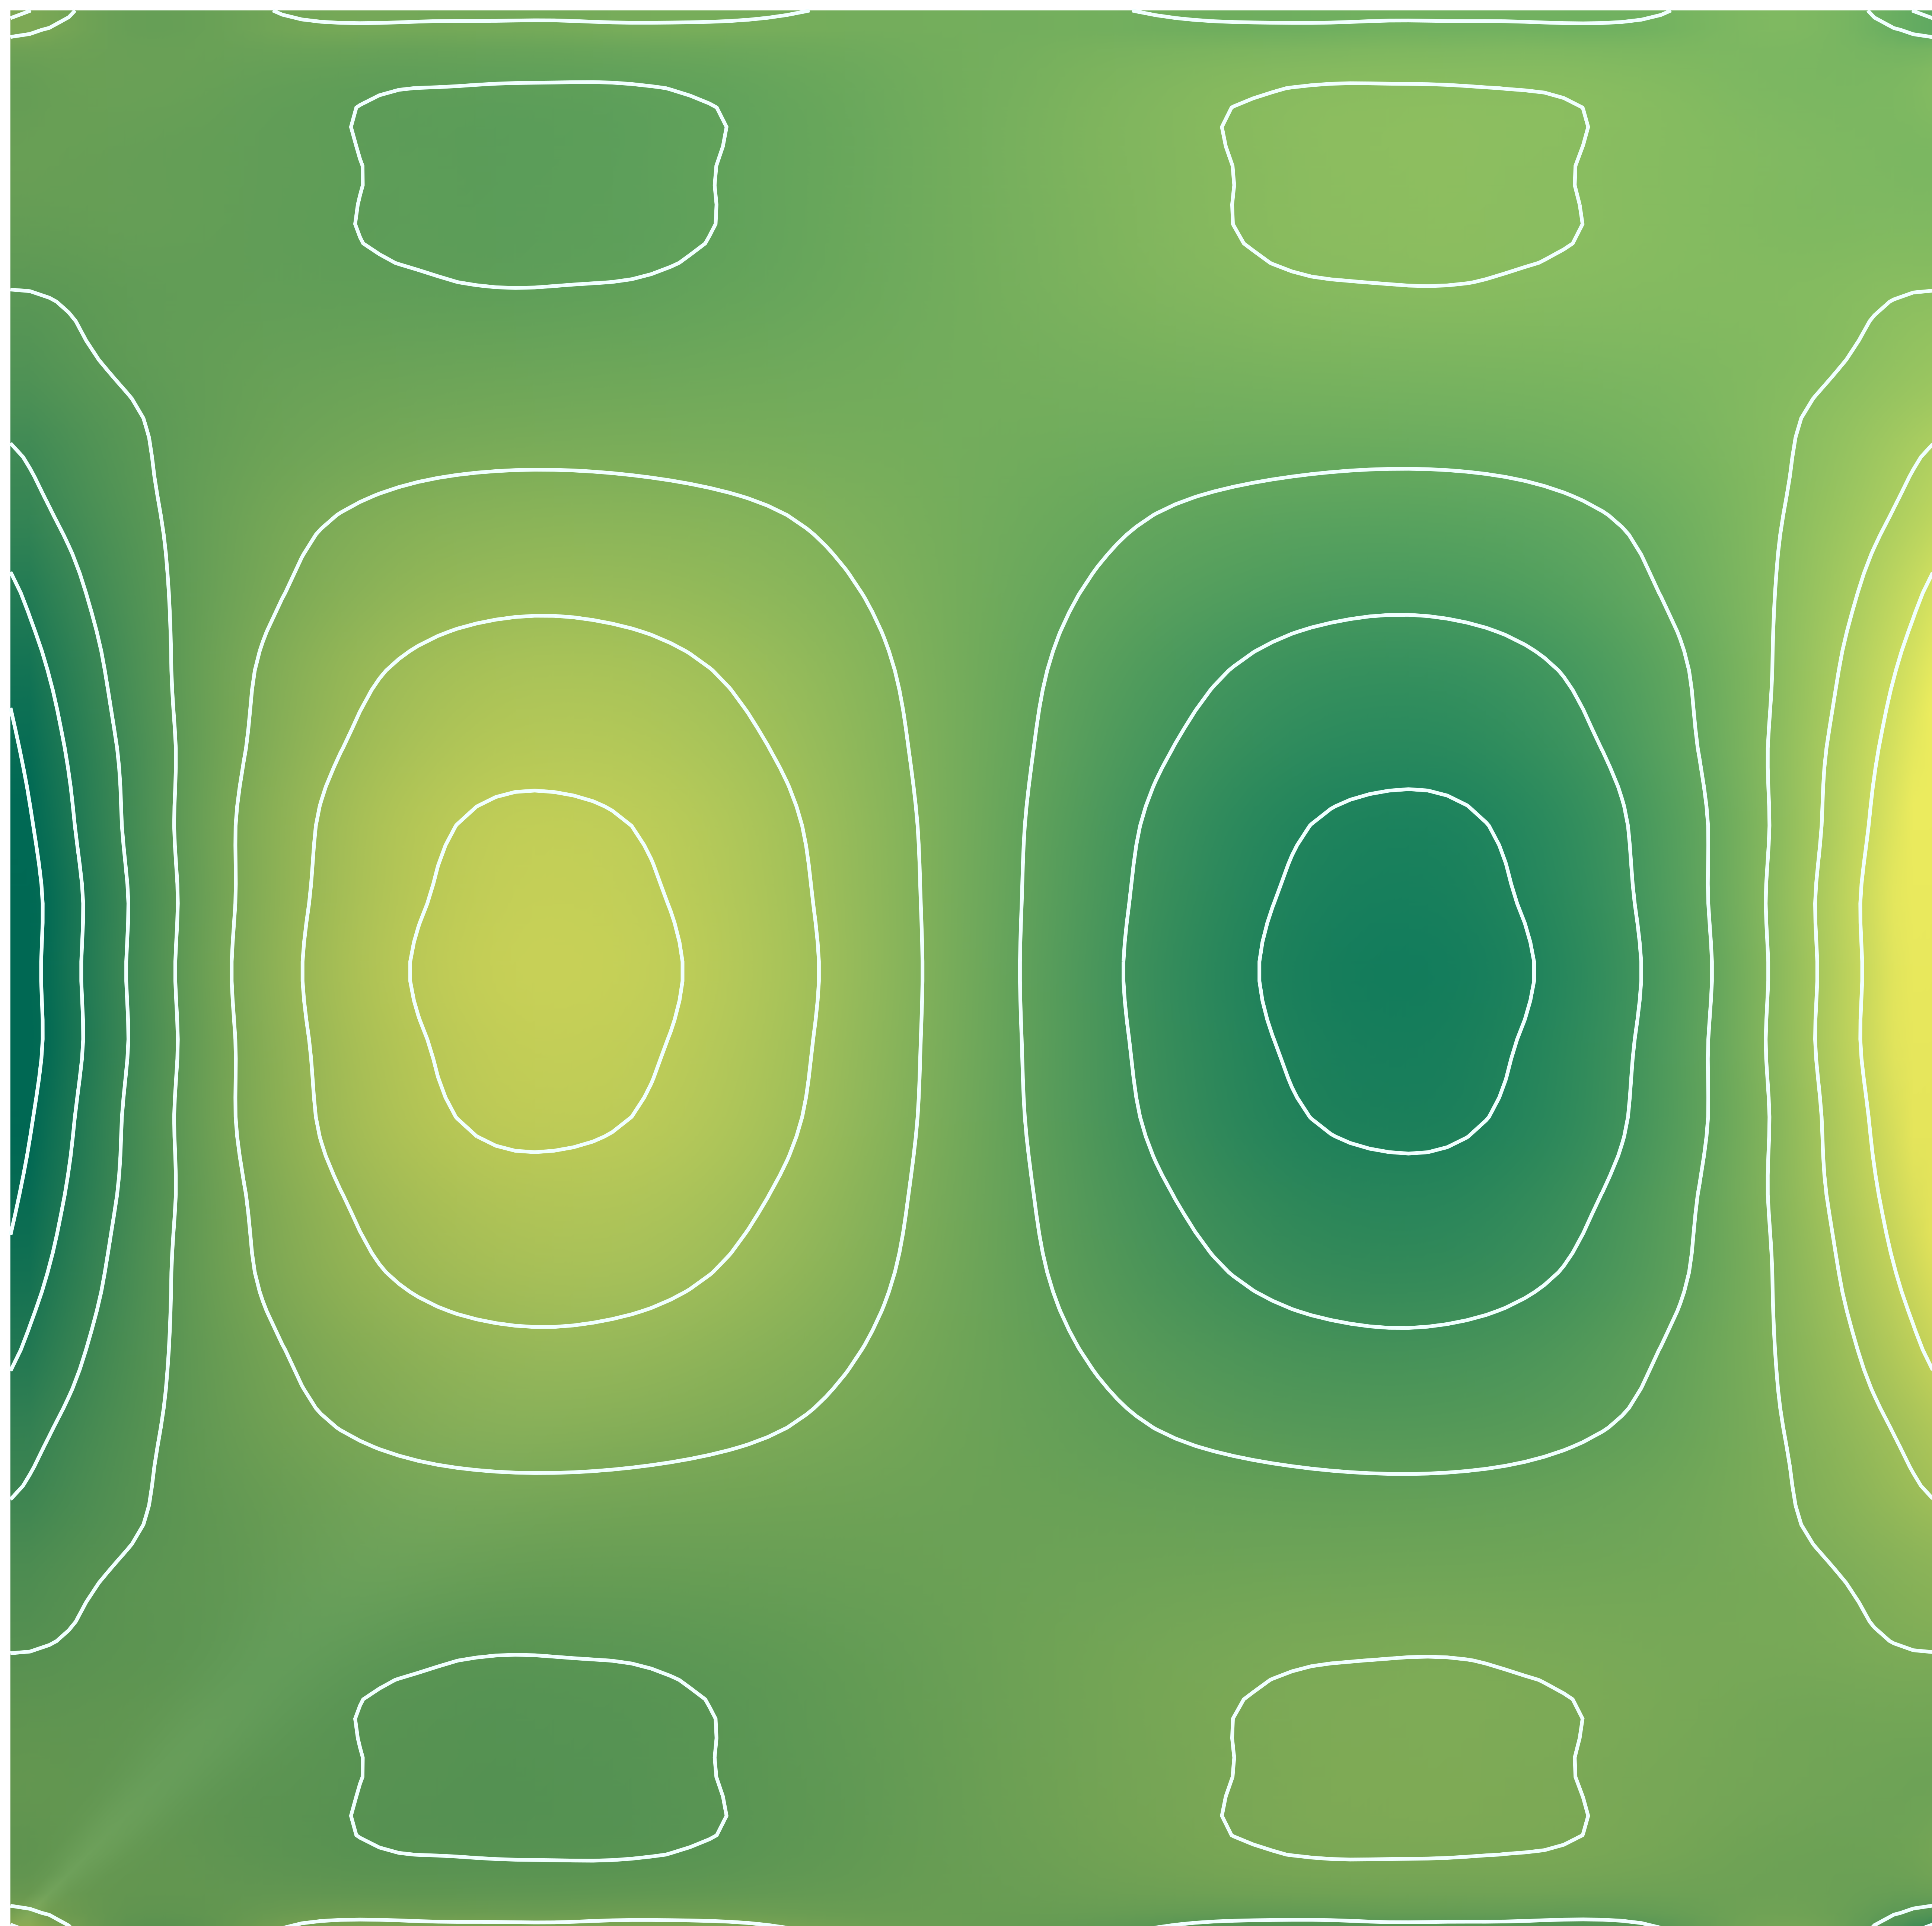
\includegraphics[width=0.4\textwidth]{figures/shearlocking/SquarePlate_mix_quad8_q1_16_14.png}}\end{subcaptiongroup}
    &\begin{subcaptiongroup}\raisebox{-0.4\height}{\includegraphics[width=0.4\textwidth]{figures/shearlocking/SquarePlate_mix_quad8_q1_16_16.png}}\end{subcaptiongroup}\\
    $3201$&\begin{subcaptiongroup}\raisebox{-0.4\height}{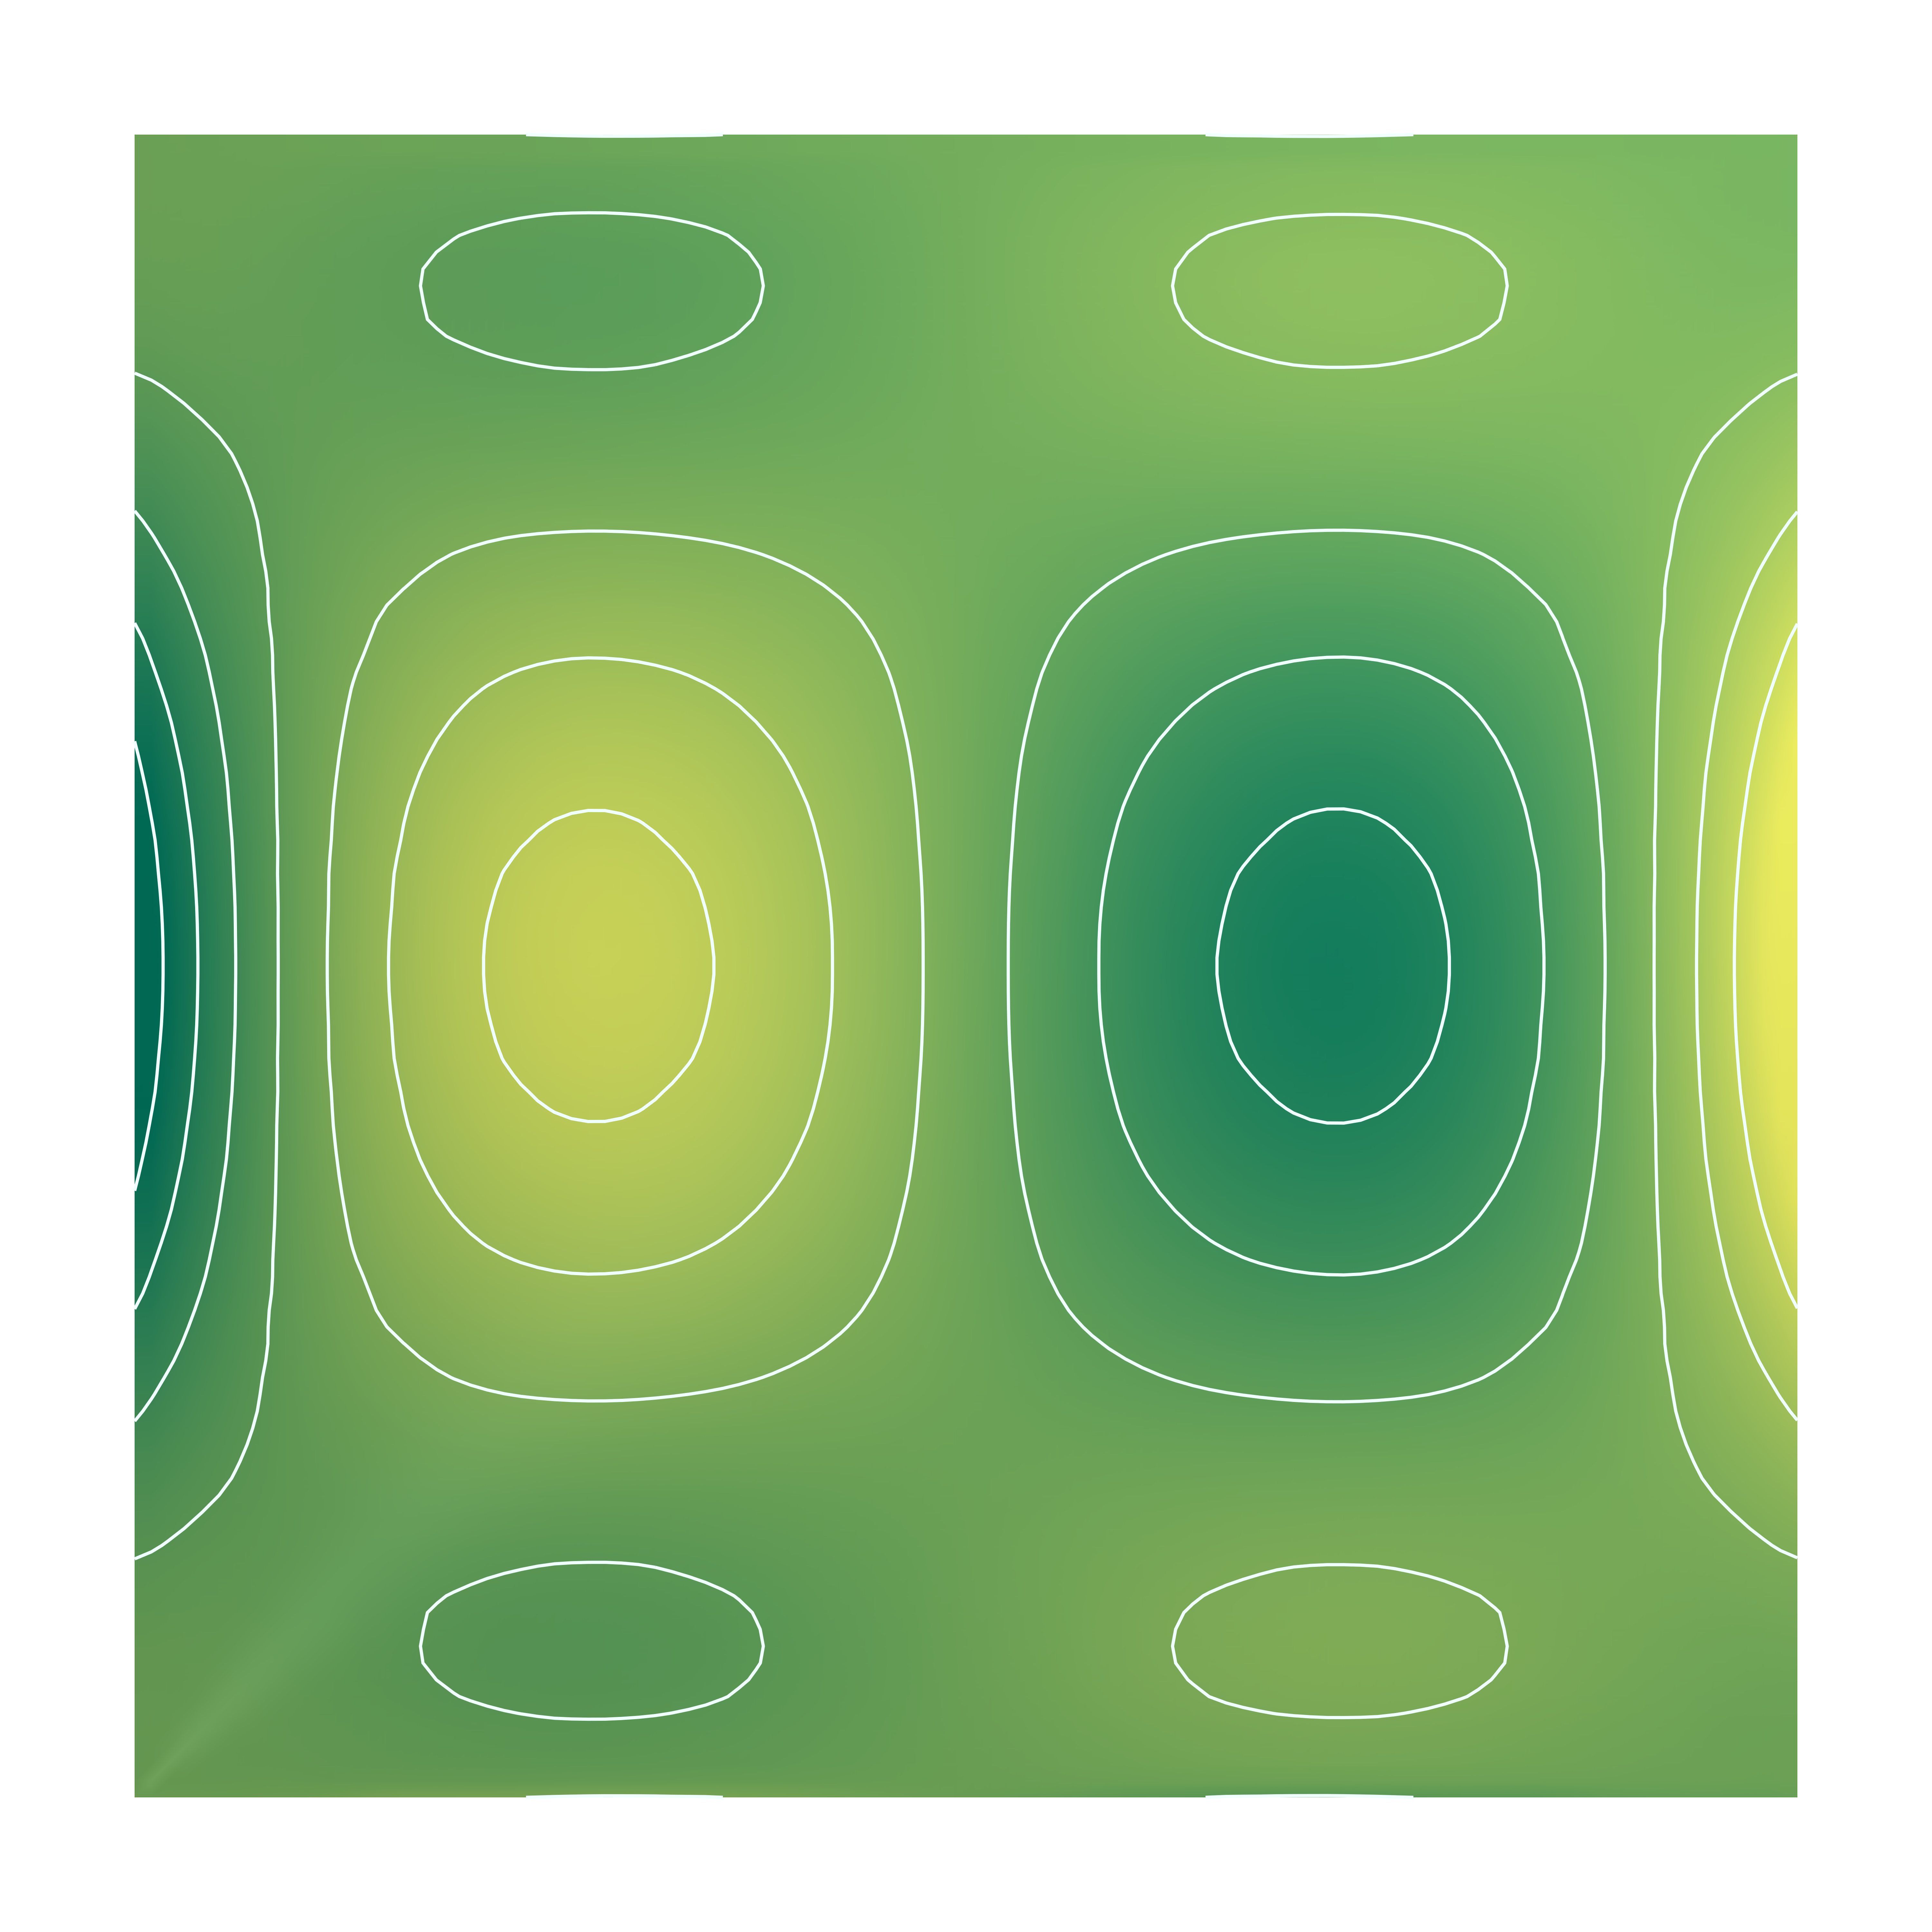
\includegraphics[width=0.4\textwidth]{figures/shearlocking/SquarePlate_mix_quad8_q1_32_26.png}}\end{subcaptiongroup}
    &\begin{subcaptiongroup}\raisebox{-0.4\height}{\includegraphics[width=0.4\textwidth]{figures/shearlocking/SquarePlate_mix_quad8_q1_32_32.png}}\end{subcaptiongroup}\\ 
    \end{tabular}
    \caption{\textbf{Quad8单元应力云图($Q_1$)}}\label{Q1-Quad8}
\end{figure}

\subsection{Morley's斜板问题}
\begin{figure}[H]
    \centering
    \begin{tabular}{cccc}
    $\quad$&最优约束比&传统约束比\\
    $1089$&\begin{subcaptiongroup}\raisebox{-0.4\height}{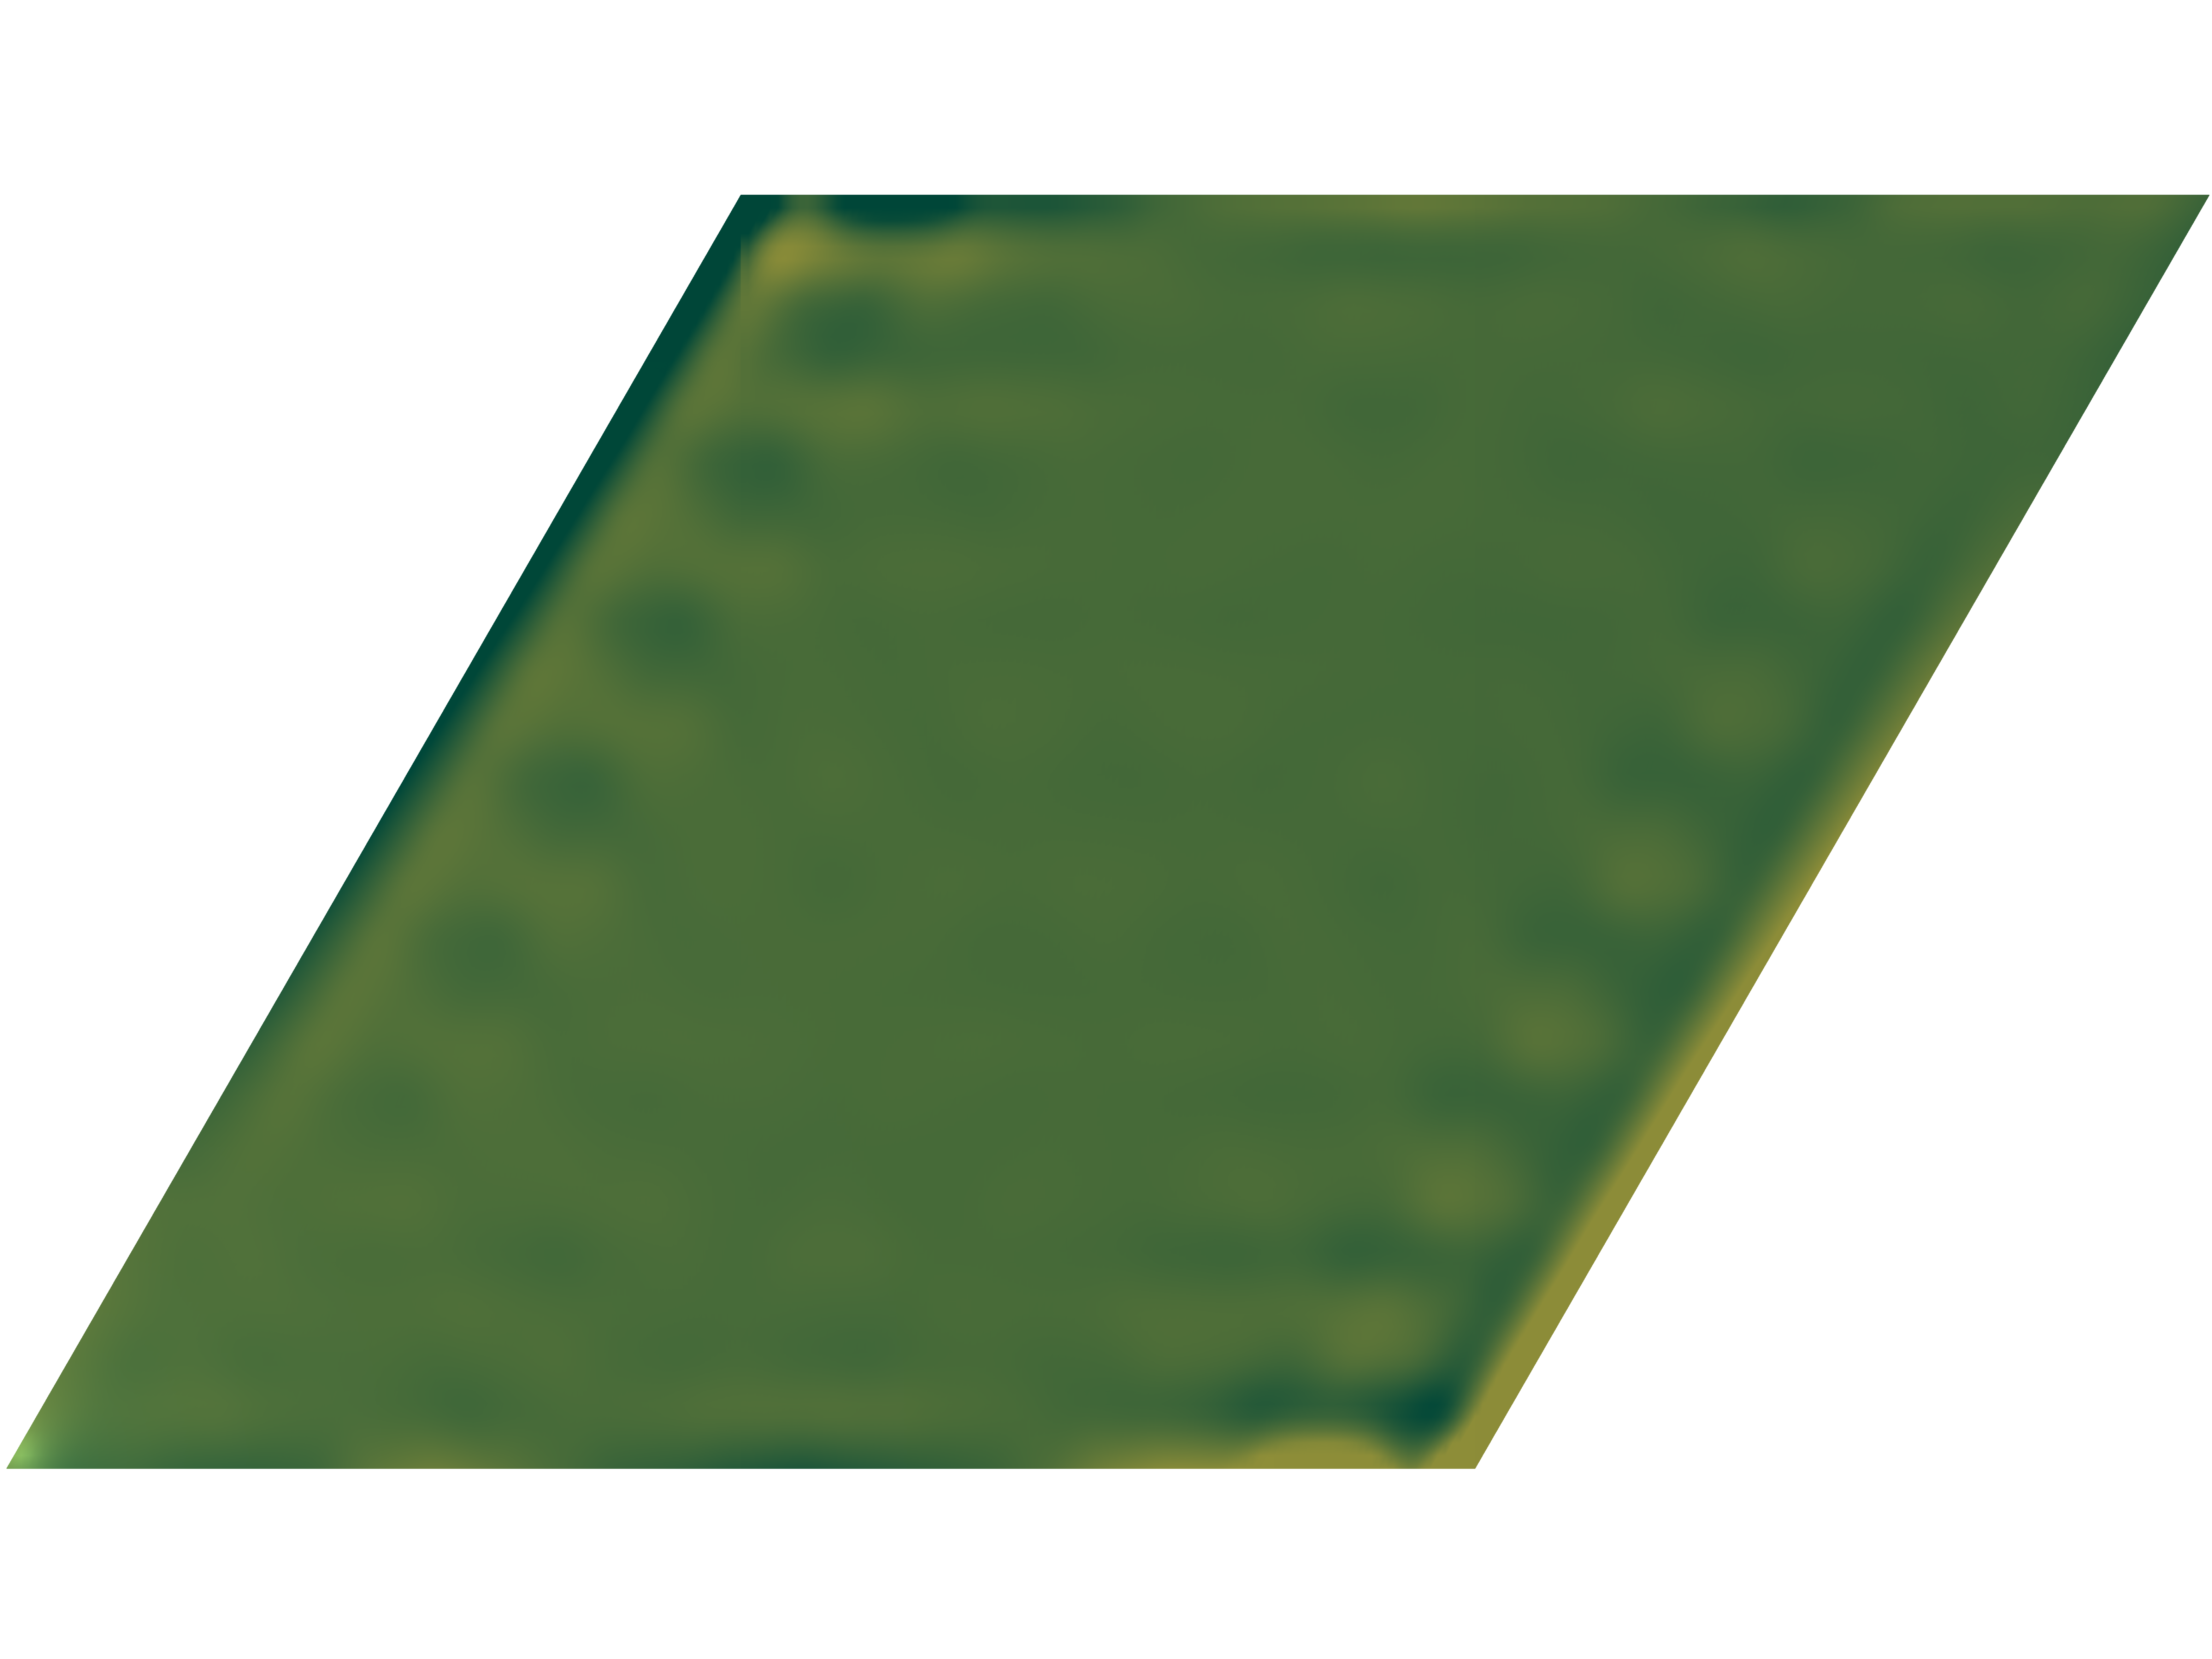
\includegraphics[width=0.4\textwidth]{figures/shearlocking/MorleysAcuteSkewPlate_tri3_q1_32_24.png}}\end{subcaptiongroup}
    &\begin{subcaptiongroup}\raisebox{-0.4\height}{\includegraphics[width=0.4\textwidth]{figures/shearlocking/MorleysAcuteSkewPlate_tri3_q1_32_32.png}}\end{subcaptiongroup}\\ 
    \end{tabular}
    \caption{\textbf{Quad8单元应力云图($Q_1$)}}\label{Q1-Quad8}
\end{figure}
\subsection{简支圆板问题问题}
